%!TEX root=../paper.tex

\chapter{Multicore Performance Variation Management on Core-level Active Timing Margin Processors}
\label{sec:process}

In this chapter, we discuss how to leverage active timing margin's automatic timing margin tracking ability to expose a multicore's static core-to-core performance heterogeneity caused by process variation, and explore how to manage the dynamically occurring inter-core frequency interference caused by the cores sharing the power delivery on an active timing margin system.

On multi-core and many-core chips, it is critical that we push down timing margin that not only deals with the dynamically occurring effects such as temperature and voltage variation but also covers the core-to-core performance heterogeneity caused by lithography's manufacturing process variation. To investigate this issue, we take the hardware active timing margin solution designed to cope with voltage noise to the next level, such as the POWER7+ multicore we experimented with in~\Sec{sec:voltage}. We study enhancing a multicore's active timing margin capability according to each core's characteristics, as well as the running applications' characteristics. We heavily instrumented the per-core hardware control loop's operation and studied its maximal efficiency gain.

By design, a chip's active timing margin implementation is usually programmable for post-silicon calibration of how aggressive the control loop should harness the available margin. If set too aggressively, active timing margin can improve power efficiency a lot, potentially at the cost of compromising execution correctness because not enough margin might be available. On the other hand, active timing margin cannot realize the full efficiency gain if it is set too conservatively. In today's practice, multicore's active timing margin configuration is usually conducted by batches in course granularity for ease of mass production, without taking into consideration the heterogeneity between cores and applications. We factor in these scenarios and investigate how to customize and manage active timing margin operation to maximize its efficiency gain.

\begin{figure}[t]
  \centering
  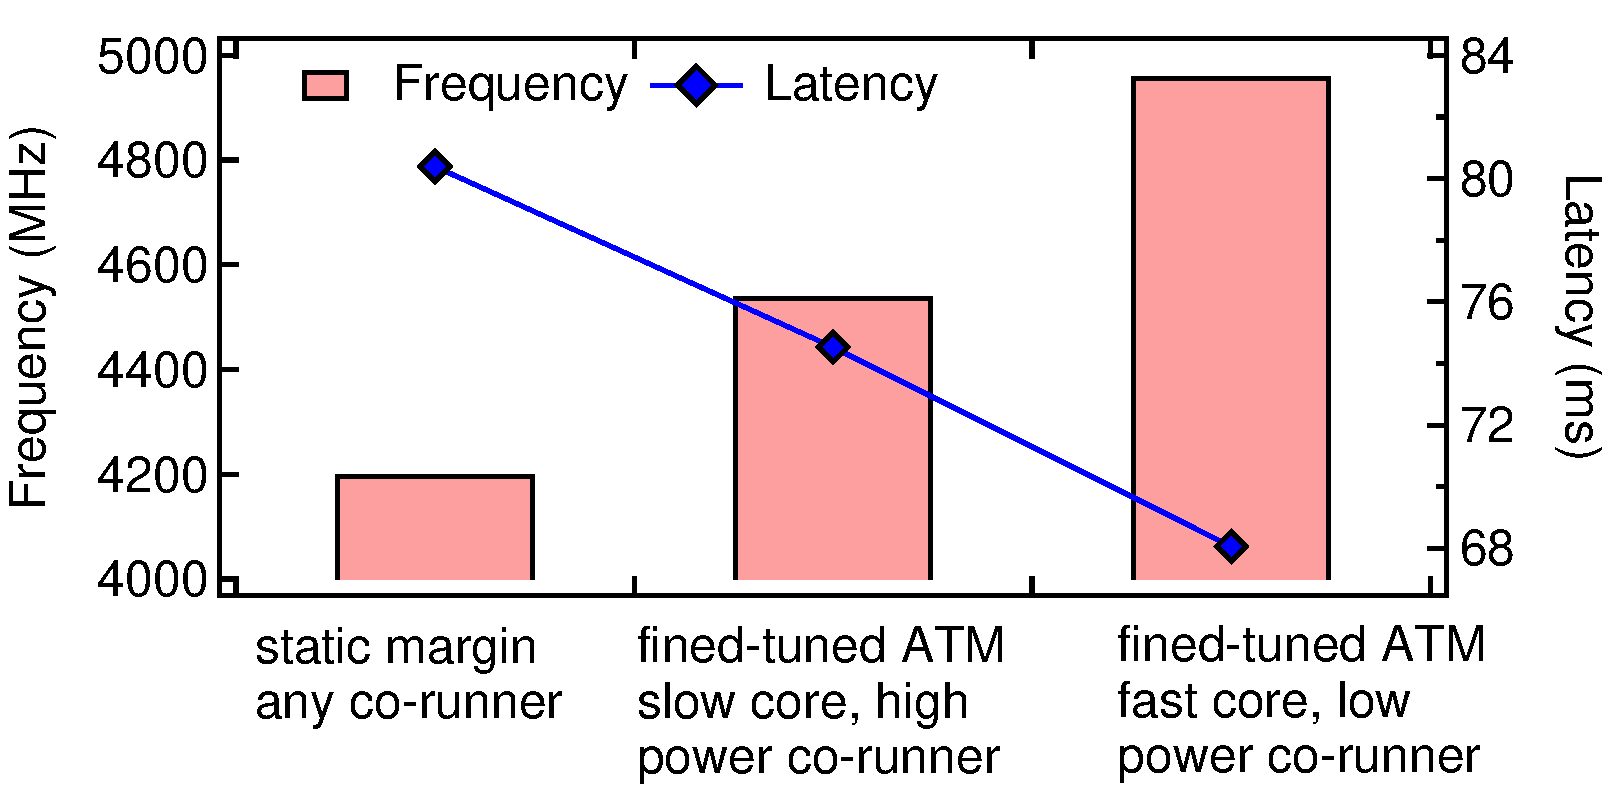
\includegraphics[trim=0 0 0 0,clip,width=.75\linewidth]{graphs/process//noisy-latency.pdf}
  \caption{\bench{SqueezeNet} inference latency on a POWER7+ core under different timing margin settings. Aggressively customizing Active Timing Margin, putting workload on to faster cores, and co-locating it with ``friendly'' low-power applications significantly enhance performance.}

  \label{fig:motivate-latency}
\end{figure}

\Fig{fig:motivate-latency} shows a POWER7+ processor core's performance under different timing margin settings~\cite{sinharoy2011power7, floyd2011introducing}. We instrument POWER7+'s active timing margin via its Critical Path Monitors (CPMs), a programmable interface of the chip's canary circuit that measures available margin~\cite{lefurgy2011active, drake2013single}. We illustrate with the inference latency of \bench{SqueezeNet}, a compressed convolutional neural network (CNN). Under conventional static timing, the chip clocks at 4.2~GHz, producing an average inference latency of 80~ms. Under the chip's default active timing margin, a poorly managed system that co-locates \bench{SqueezeNet} with high-power co-runners such as \bench{daxpy} increases frequency to 4.4~GHz, yielding a limited 3.75\% performance improvement. However, customizing each core's active timing margin and wisely managing the system to let \bench{SqueezeNet} run alone boosts core frequency to 5~GHz and reduces latency by 15\%, a 4X the performance gain over the default production system.

Inspired by the benefits shown in~\Fig{fig:motivate-latency}, we set out to systematically customize each core's \emph{Active Timing Margin}, with the goal of extracting useful insights on active timing margin operation that will guide overall system level performance and power management. Although our work is conducted on an IBM POWER7+ server, the insights we gathered apply to other active timing margin systems as the knobs we instrument exist for all active timing margin implementations.

\section{Customizing Active Timing \\Margin Operation}
\label{sec:process:configurability}

In our study, we convert all of active timing margin's reclaimed timing margin into frequency and keep $V_{dd}$ unchanged. This process bypasses the restriction on undervolting wherein a chip's worst-case core limits the amount of undervolting. Overclocking allows each core to independently adapt to its conditions and can fully expose a chip's inter-core speed differential, potentially producing more performance benefit. We let active timing margin boost each core's frequency at $V_{dd}$ 1.25~V, the 4.2~GHz P-state.

We explain how to customize a multicore's active timing margin operation to be more aggressive, which extracts more timing margin and increases frequency. Reconfiguring active timing margin's control loop to its operating limit is unexplored before, thus we propose a systematic procedure to characterize how the processor behaves under different scenarios and timing margin reclamation levels. The insights we gain when executing this procedure is instrumental in deploying customized active timing margin systems in production.

%We find active timing margin's operating limits vary between different workload scenarios, so a comprehensive procedure is needed to thoroughly profile active timing margin's reconfiguration and quantify the factors that affect its operating limits. We believe our approach sets the foundation for bringing out an active timing margin core's full performance and exposing the core-to-core speed variation.

\subsection{Programming Critical Path Monitors \\to Reconfigure Margin Reclamation}
\label{sec:process:configurability:howto}

\begin{figure}[t]
  \centering
  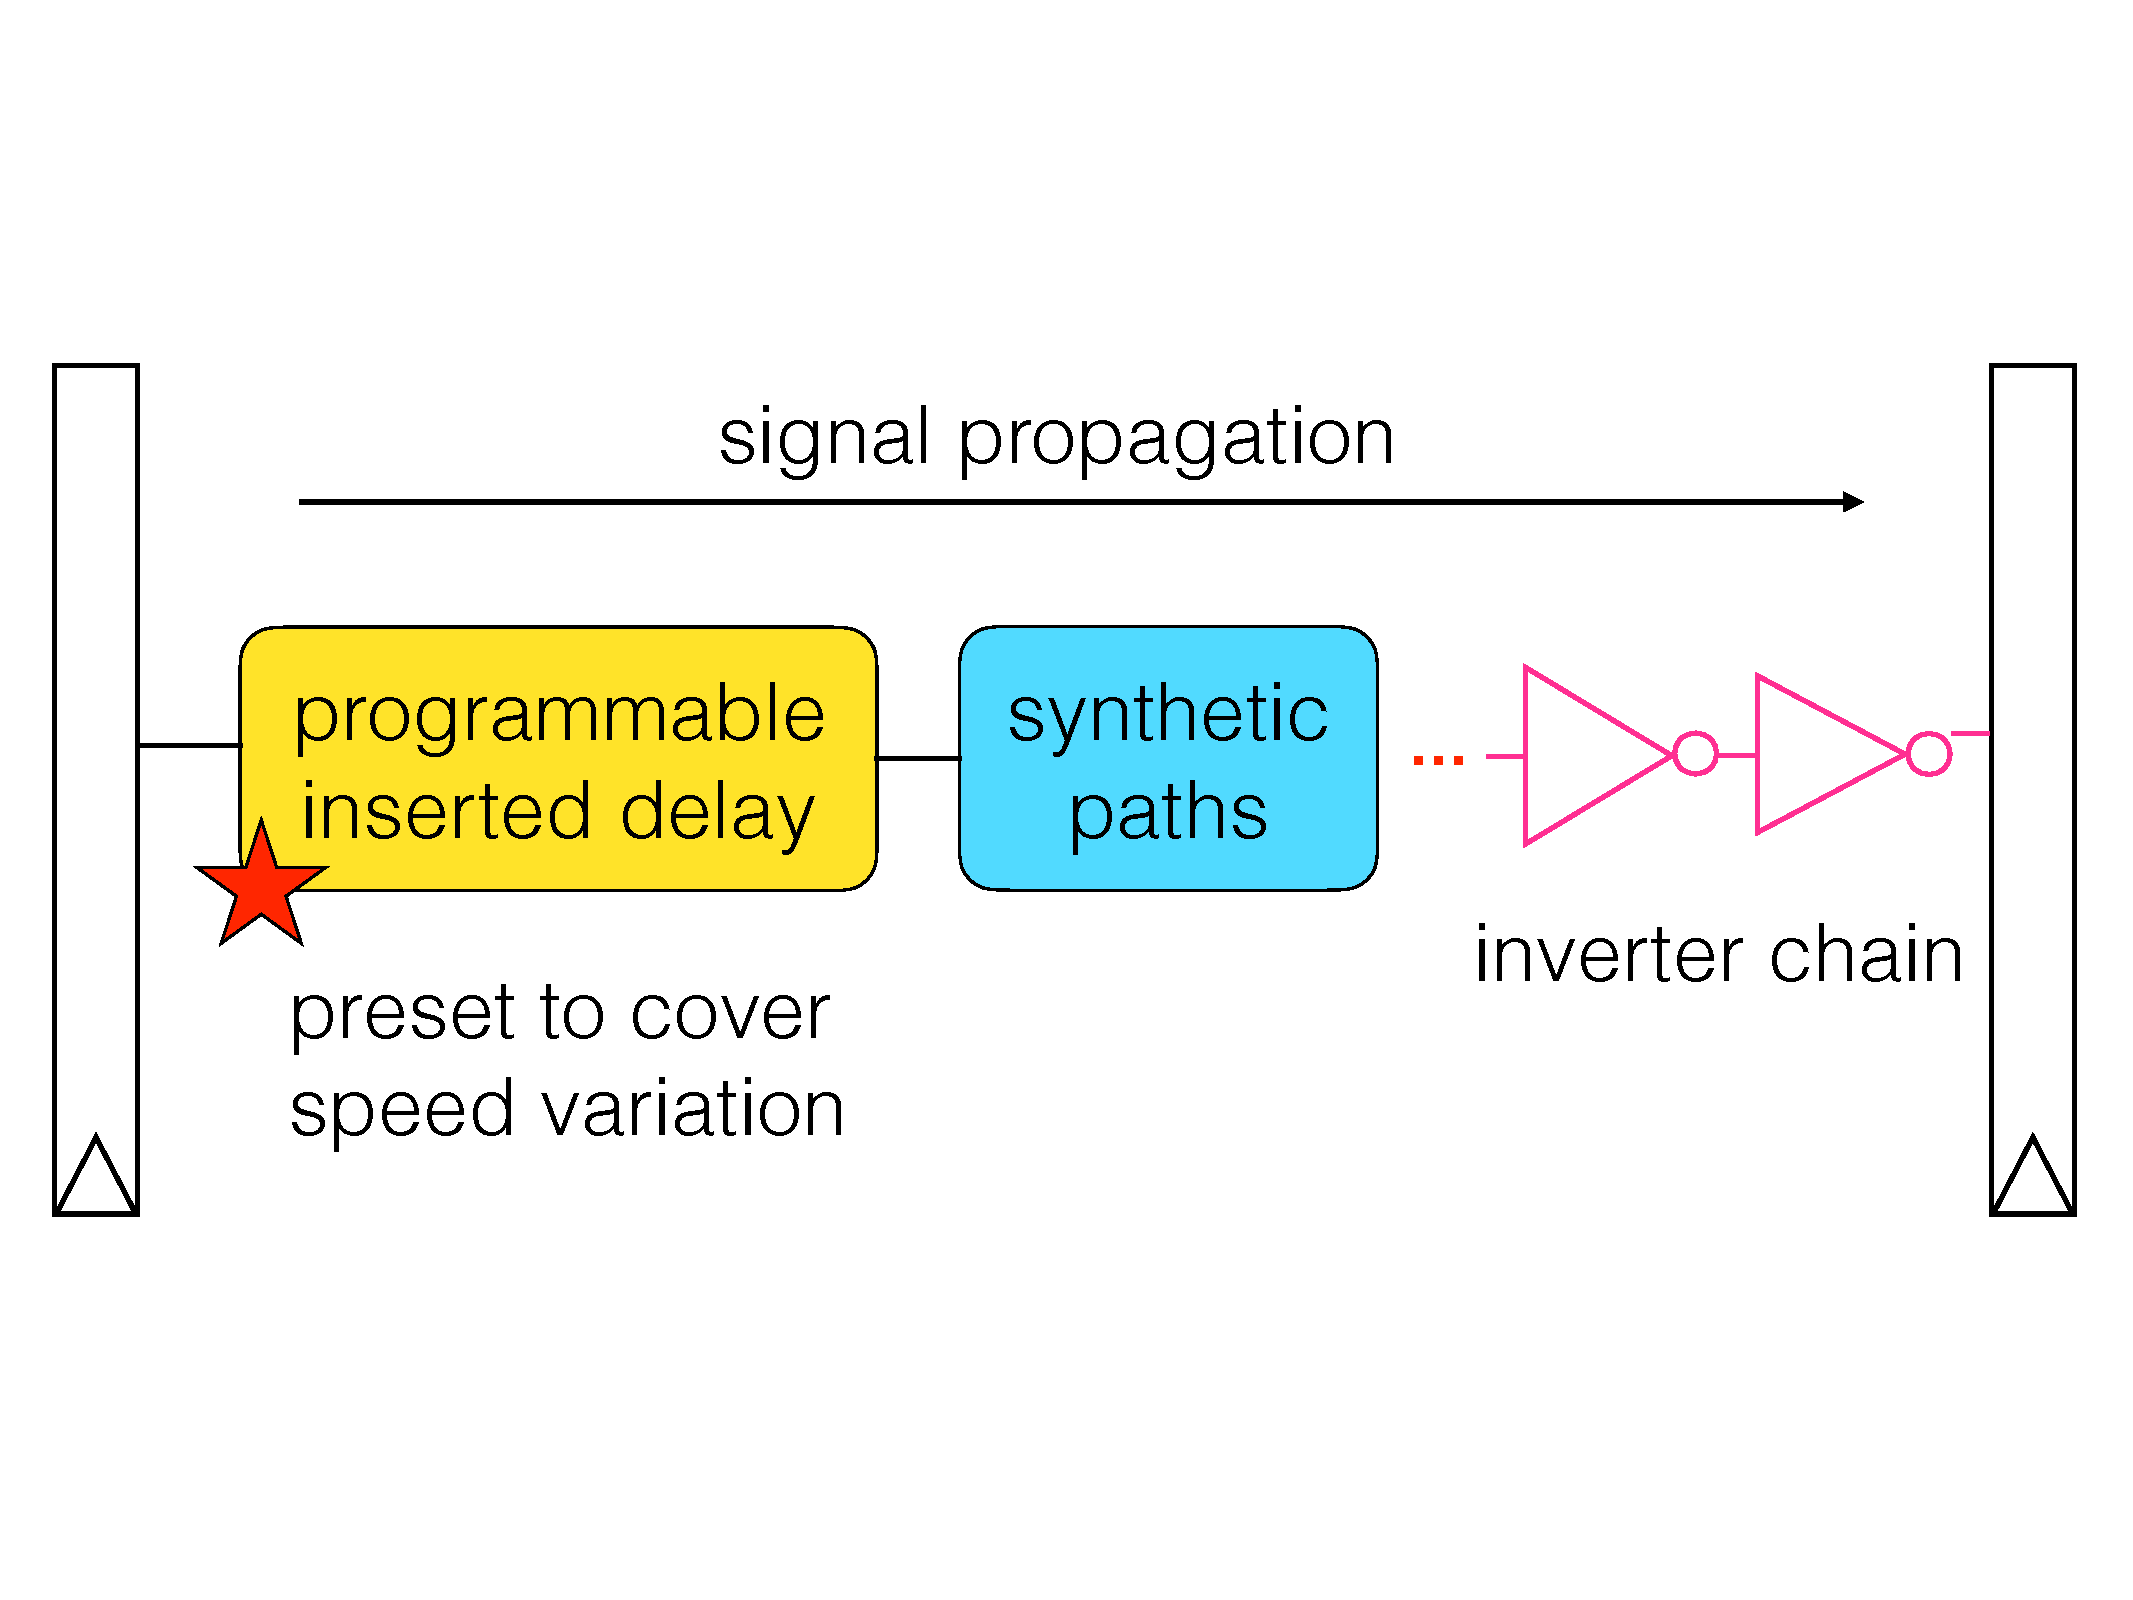
\includegraphics[trim=0 210 0 190,clip,width=0.8\linewidth]{graphs/process//cpm-struct.pdf}
  \caption{CPM structure: programming the inserted delay affects the timing it takes to travel to the inverter chain, and sets the margin sensed counted by the inverters.~\cite{drake2007distributed, drake2013single}
  \label{fig:cpm-struct}
  }
\end{figure}

We use the POWER7+'s programmable Critical Path Monitors (CPMs) to control the active timing margin's operation aggressiveness. \Fig{fig:cpm-struct} illustrates the mechanism. A CPM uses three stages to measure timing margin: (1)~inserted delay, (2)~synthetic paths, and (3)~an inverter chain. The inserted delay is a configurable circuit. A user can specify the number of inverters a signal pass through to select its timing delay length. The synthetic path simulates a pipeline circuit's delay with a set of paths, including AND, OR, and XOR gates and wires. The final inverter chain quantifies the time left after the signal propagates past the inserted delay and synthetic path by counting the number of inverters a signal passes. The inverter count is a CPM's final output and is sent to the DPLL for clock adjustment.

\begin{figure}[t]
    \centering
    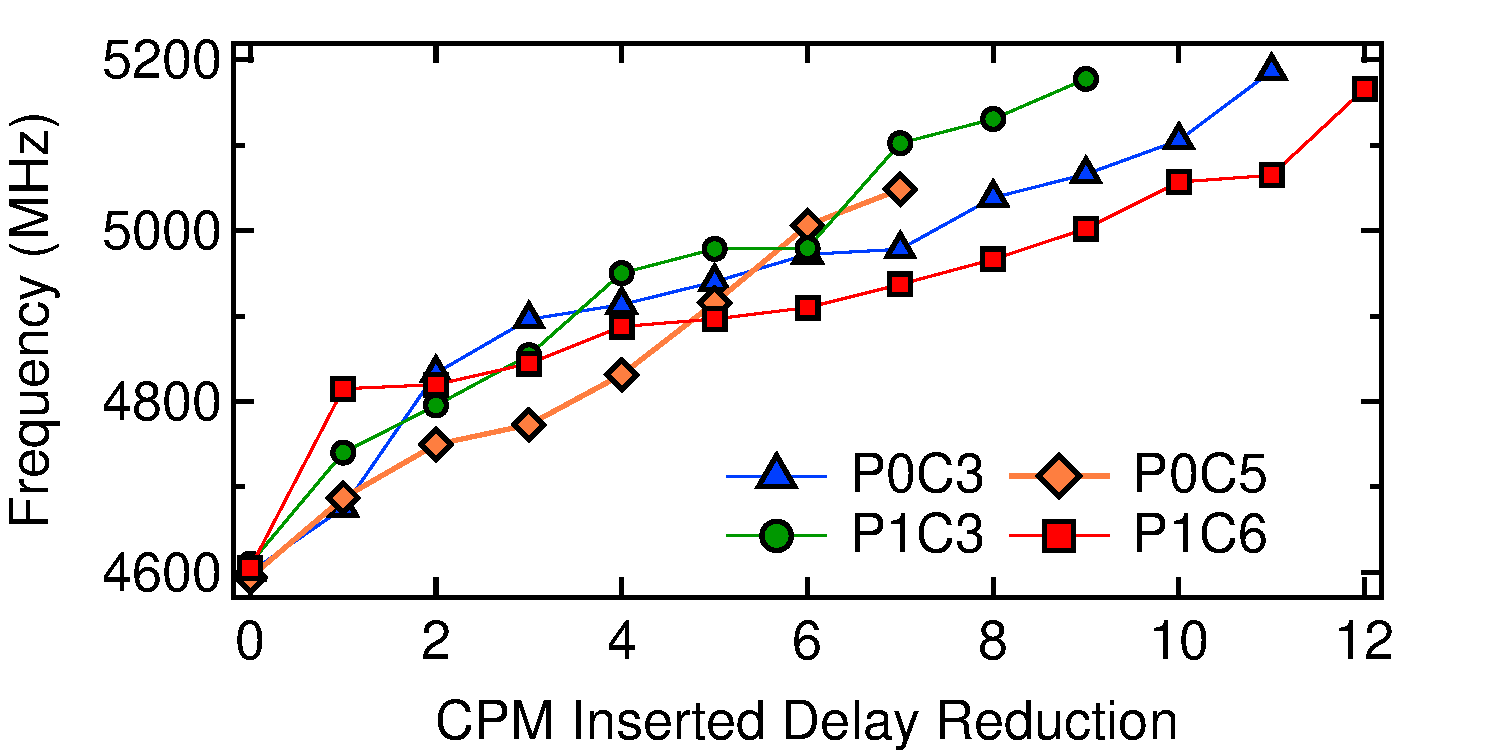
\includegraphics[trim=0 0 0 0,clip,width=.8\linewidth]{graphs/process//delay-freq.pdf}    
    \caption{Reducing inserted added delay makes the CPM count more time margin after a signal travels through the synthetic path. The DPLL then increases frequency to harvest the excess margin reported by CPM's inverter chain.}
    \label{fig:delay-freq}
\end{figure}

By programming the inserted delay to different values, active timing margin's perception of the amount of available timing margin changes, and thus it is induced to become more or less aggressive in reclaiming timing margin. \Fig{fig:delay-freq} shows, for four example cores (C), across two processors (P) on the same system, how active timing margin converts more margin into frequency as the CPM inserted delay is reduced. The default delay (normalized to 0) makes active timing margin push core frequency to around 4.6~GHz, but reducing inserted delay (reduction steps beyond 0) pushes frequency to over 5~GHz, a 20\% improvement over the static timing margin baseline. Programming the inserted delay to a smaller value (higher delay reduction) decreases the time to the end of the synthetic path, leaving more margin to be counted by the inverter chain. The DPLL loop harnesses the excess margin by overclocking.

Before a POWER7+ processor is shipped, each CPM's inserted delay is configured with some default ``protection'' delay to keep the CPM timing margin conservative, which guarantees correct active timing margin execution. The protection delay also smooths out the speed differences between different corners of a chip. For the 64 CPMs in our two-socket system (we exclude CPMs in the LLC because it lies in a different clock domain), the protection delays range from 7 to 20, nearly a 3X range, indicating significant silicon speed variation.

In the POWER7+, we configure the inserted delay by programming it with a discrete step count through the server's accompanying service processor. Each step represents some amount of timing delay. Under the static margin at 4.2~GHz, reducing the inserted delay by one step lets the CPM detect one to three units more timing margin, equivalent to the speed variation caused by 20-60~mV $V_{dd}$ difference~\cite{drake2013single,zu2015adaptive}.

We reduce each core's CPM delay from the default amount to increase active timing margin aggressiveness. To simplify the exploration space, we reduce the four CPMs within a core (excluding the LLC CPM) by the same amount.

\subsection{Characterizing active timing margin Limits}
\label{sec:process:methodology}

As shown by \Fig{fig:delay-freq}, active timing margin has great potential for more aggressive operation to achieve higher frequency. But to unlock active timing margin's full potential, we need a methodology to characterize the system. \Fig{fig:methodology} outlines our procedure. 

We profile an active timing margin chip on a per-core basis. System idle is our starting point for the analysis; micro-benchmarks (uBench) cover major paths in a core; and single-threaded benchmarks representing real use cases.

\begin{figure}[H]
  \centering
  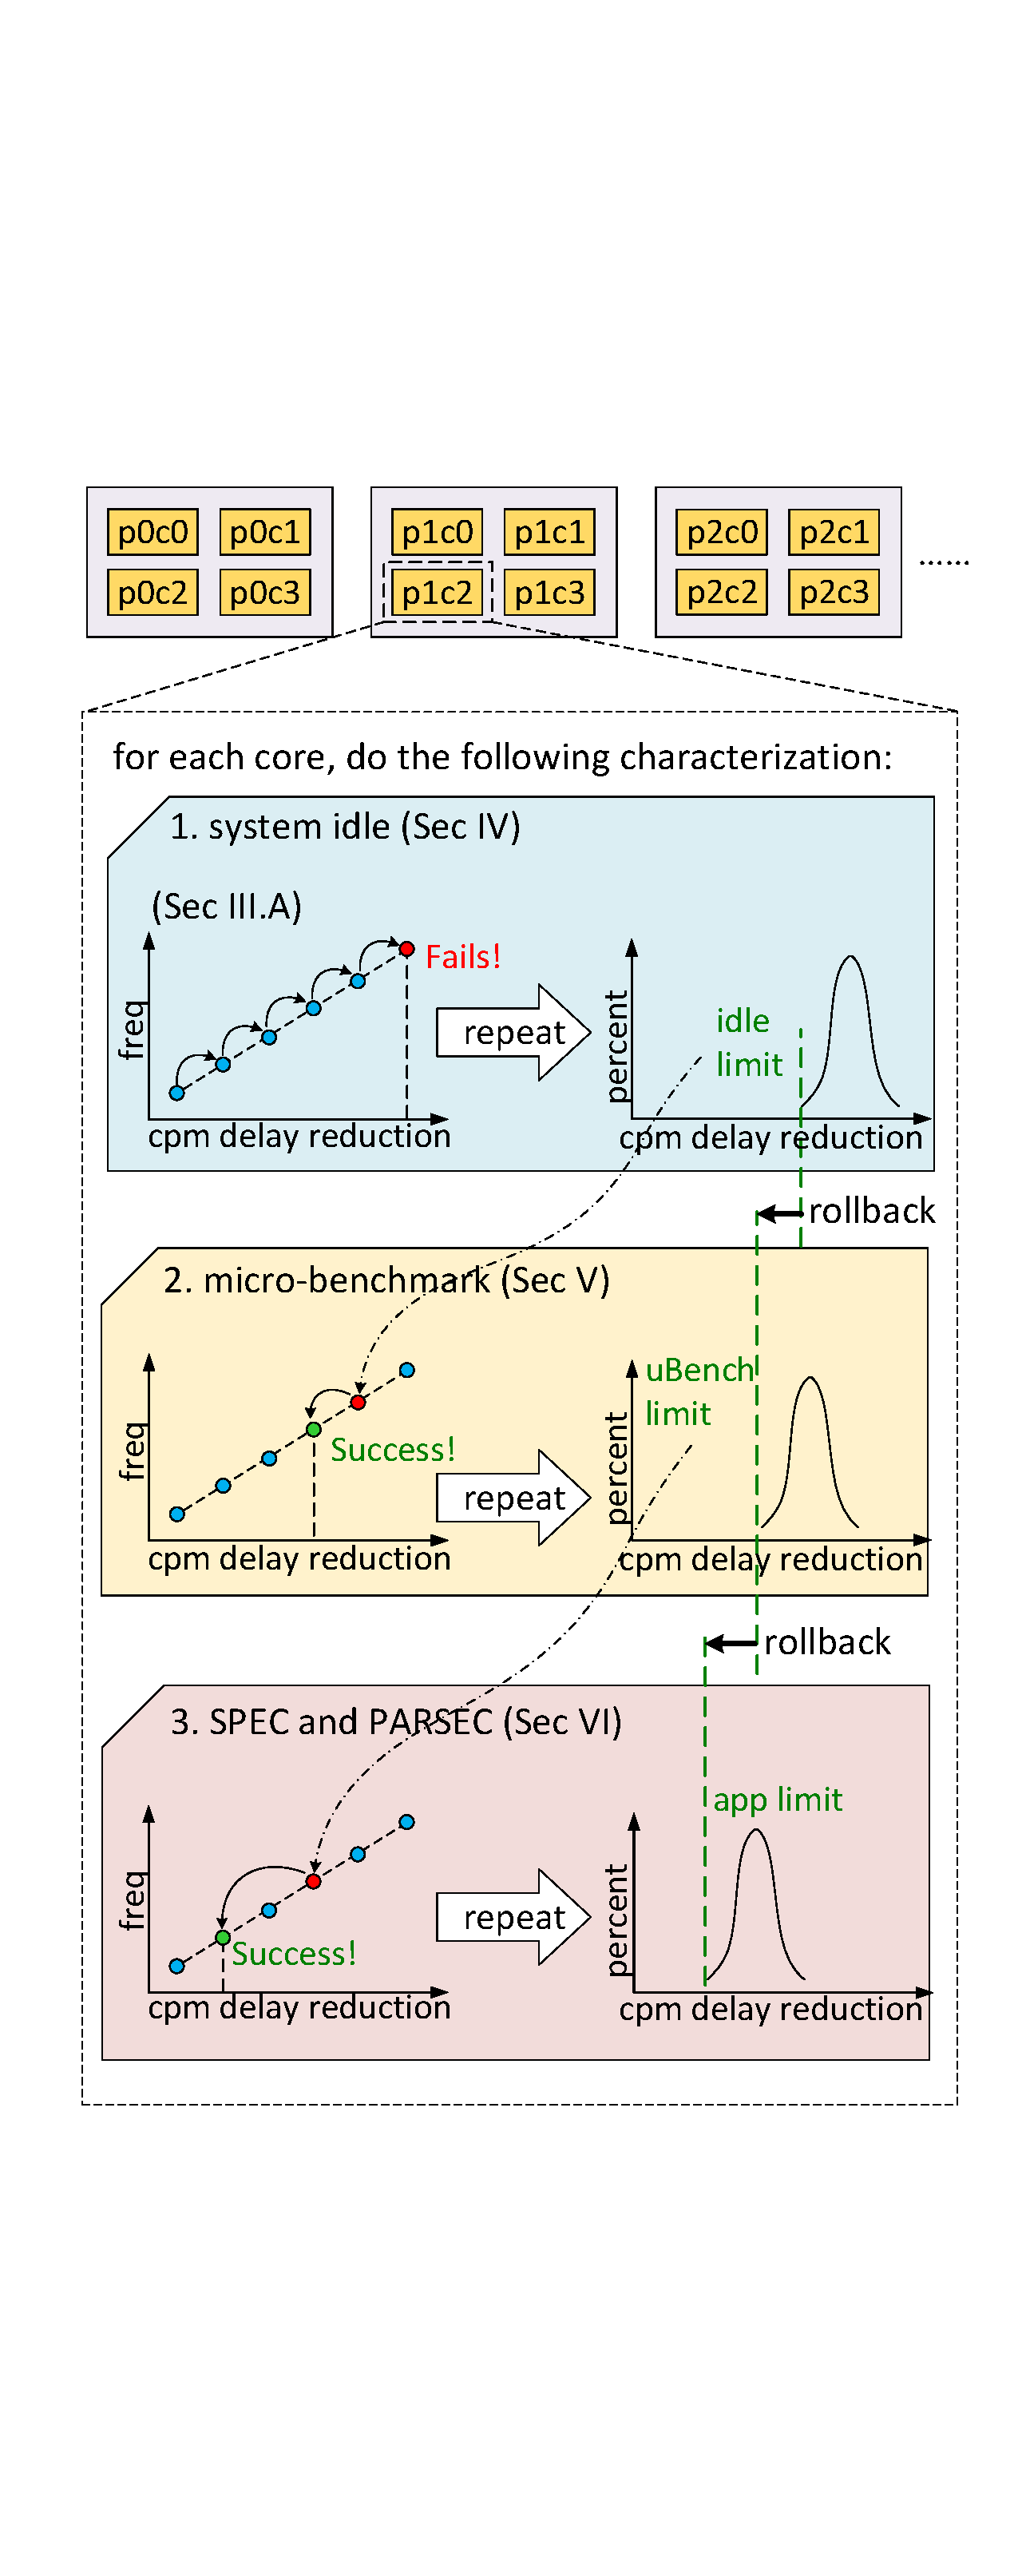
\includegraphics[trim=10 280 10 280,clip,width=.8\linewidth]{graphs/process//profile-flow/profile-flow.pdf}
  \caption{Our active timing margin characterization methodology iterates over each core and follows a step-by step approach, going from the simplest system idle scenario to the complex real-world workloads.}
  \label{fig:methodology}
\end{figure}

\textbf{System Idle} Running background operating system tasks, an idle system imposes the least stress on the processor. {Understanding each core's active timing margin operating limits under system idle provides us with valuable insight into inherent core-to-core differences.}

\textbf{Micro-benchmarks (uBench)} Traditionally, micro-benchmarks are used to measure the performance of individual processor modules, such as the branch predictor, floating point unit, and caches. In active timing margin, micro-benchmarks serve an additional purpose because each one primarily touches only one part of the core, avoiding complex microarchitectural interactions. We thus use uBench to get a more comprehensive profile of core-to-core microarchitecture level variation.

\begin{figure*}[t!]
      \subfloat[p0 core 0.] {
        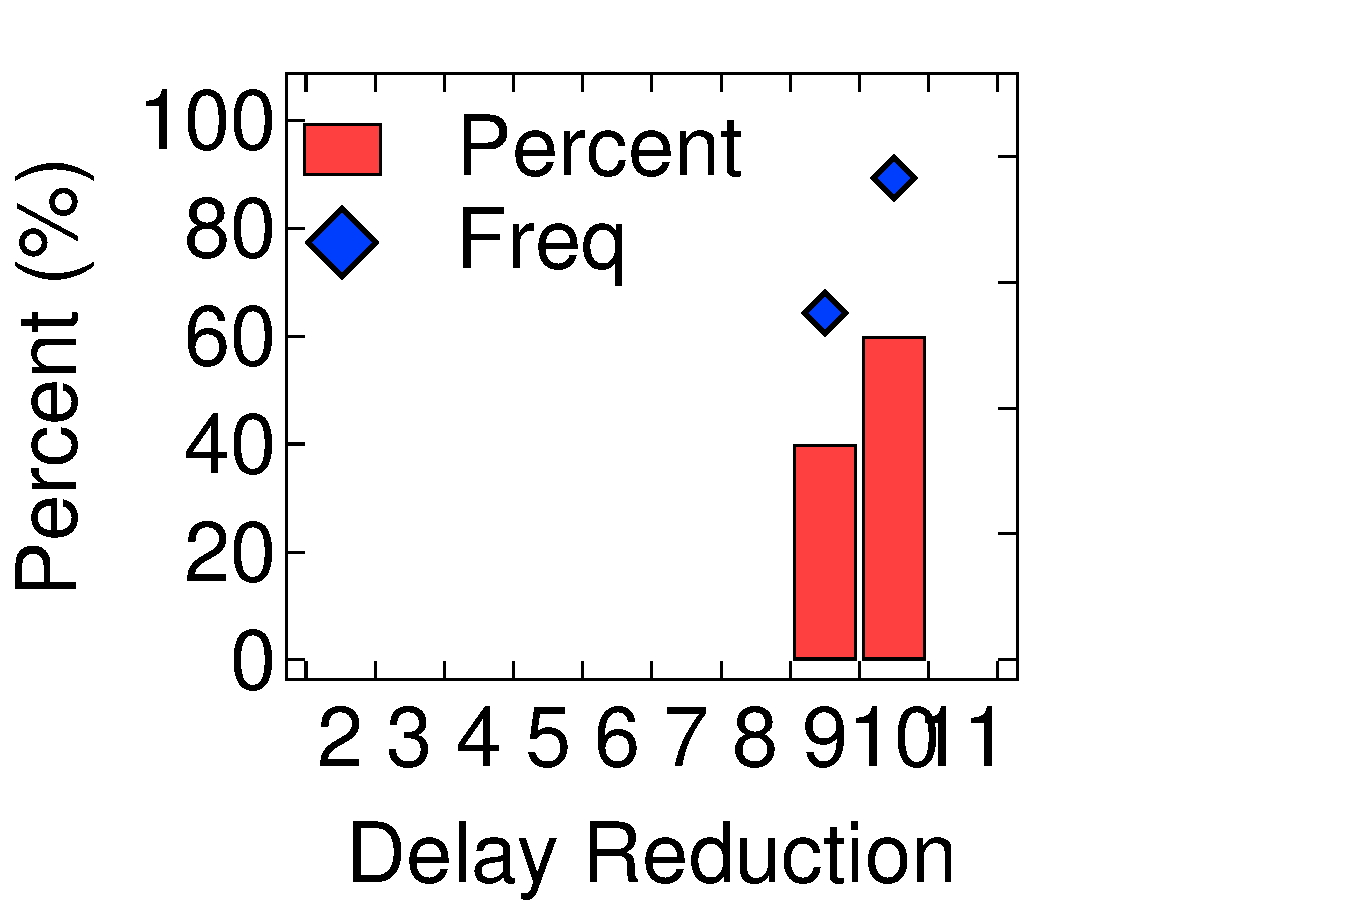
\includegraphics[trim=0 0 0 0,clip,width=.23\linewidth]{graphs/process/idle-limit-dist/idle-limit-dist-p0c0.pdf}
        \label{fig:idle_dist_p0c0}
      }
      \hfill
      \subfloat[p0 core 1.] {
        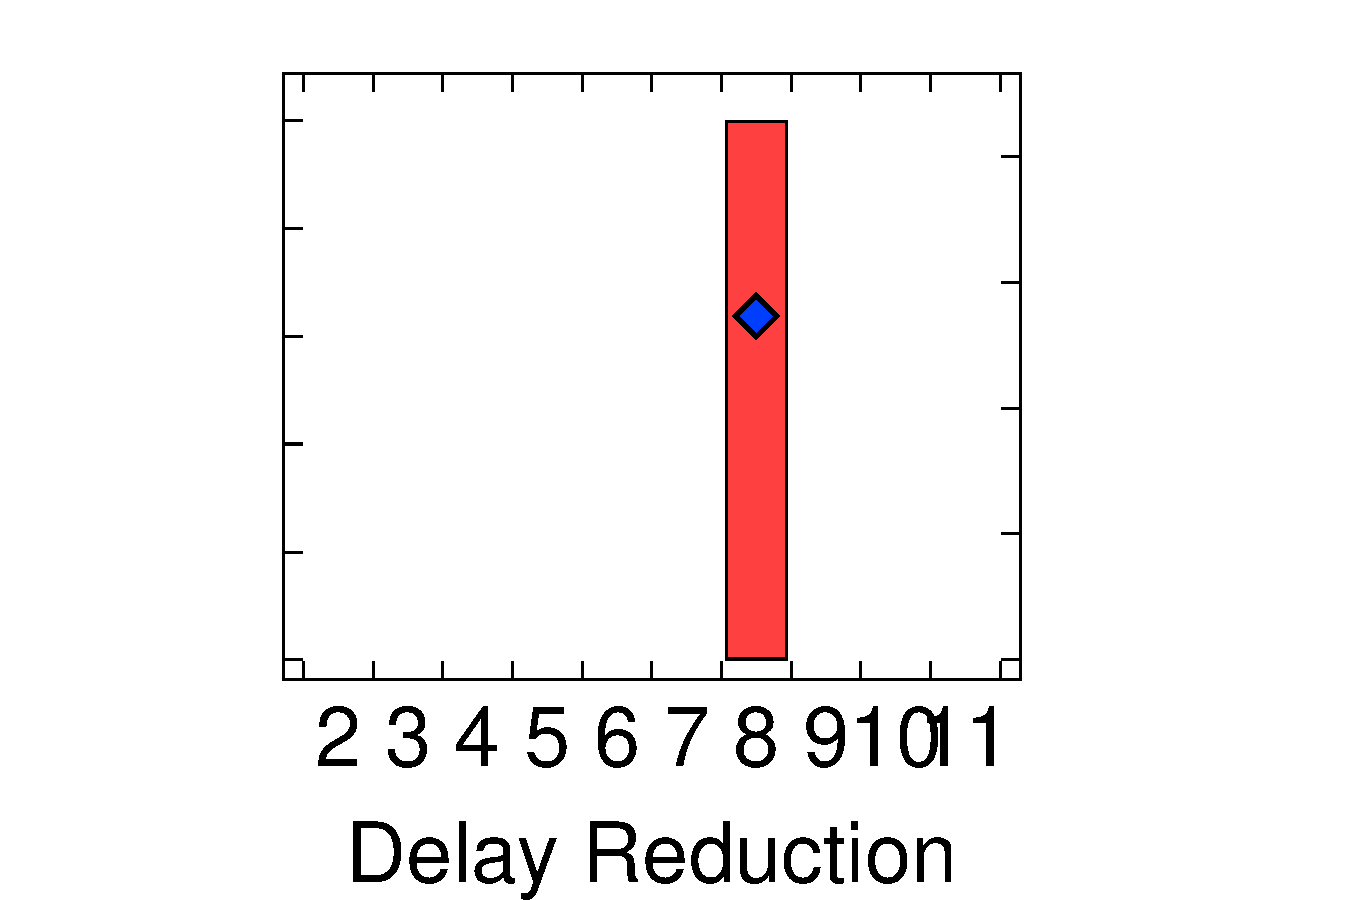
\includegraphics[trim=0 0 0 0,clip,width=.23\linewidth]{graphs/process/idle-limit-dist/idle-limit-dist-p0c1.pdf}
        \label{fig:idle_dist_p0c1} 
      }
      \hfill
      \subfloat[p0 core 2.] {
        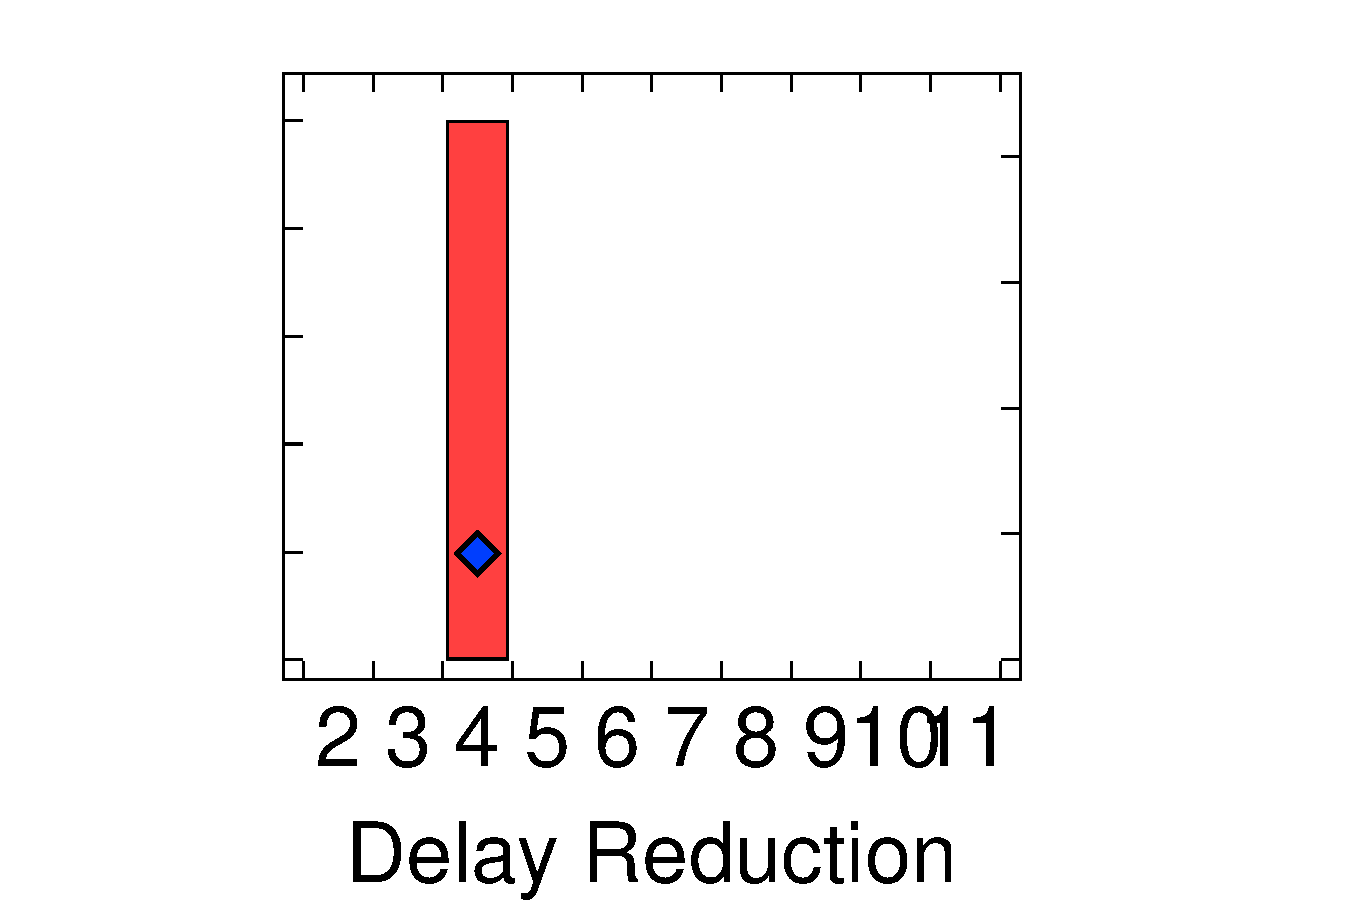
\includegraphics[trim=0 0 0 0,clip,width=.23\linewidth]{graphs/process/idle-limit-dist/idle-limit-dist-p0c2.pdf}
        \label{fig:idle_dist_p0c2} 
      }
      \hfill
      \subfloat[p0 core 3.] {
        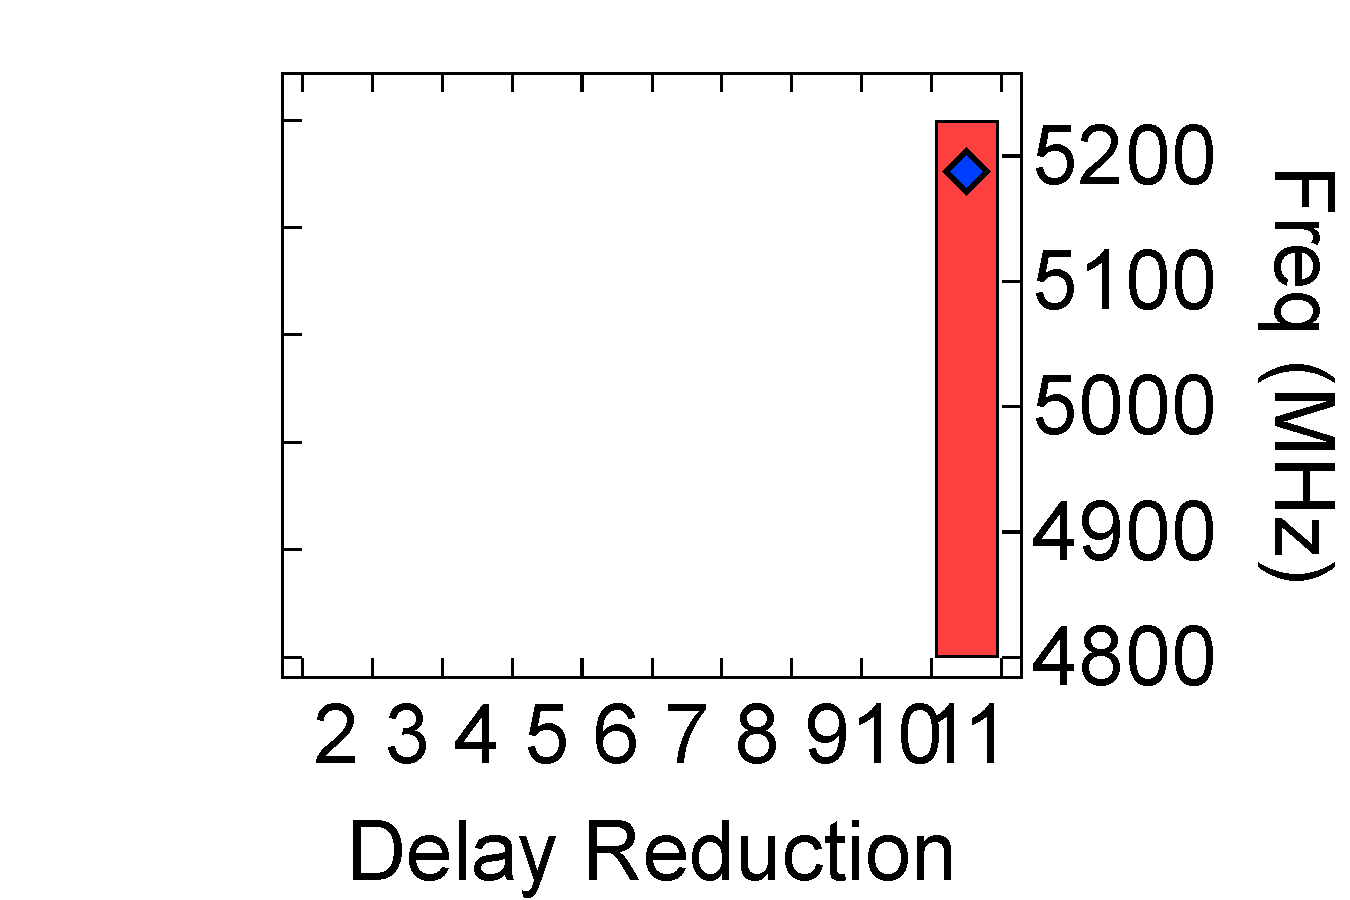
\includegraphics[trim=0 0 0 0,clip,width=.23\linewidth]{graphs/process/idle-limit-dist/idle-limit-dist-p0c3.pdf}
        \label{fig:idle_dist_p0c3} 
      }

      \subfloat[p0 core 4.] {
        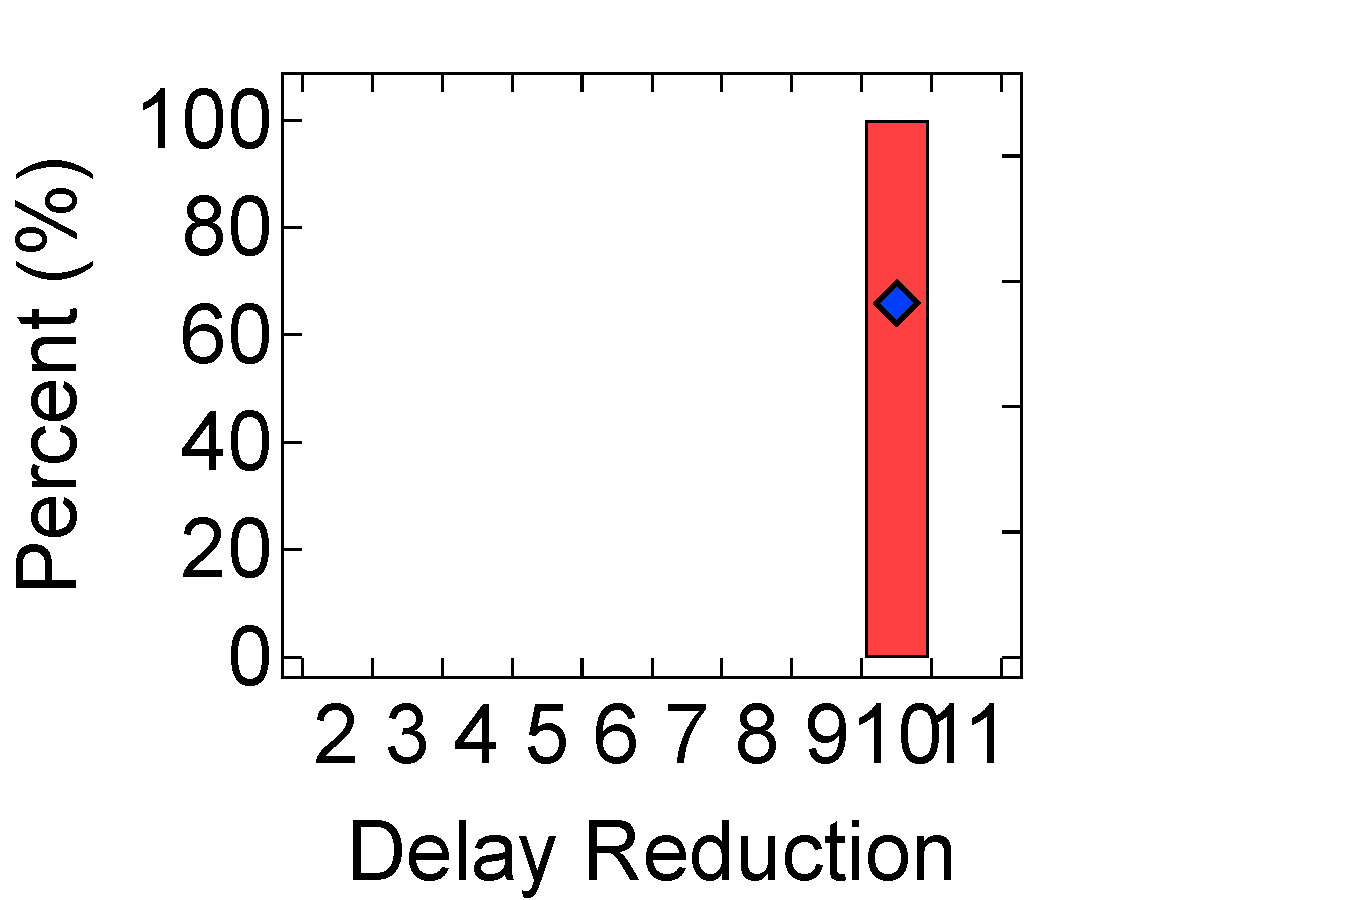
\includegraphics[trim=0 0 0 0,clip,width=.23\linewidth]{graphs/process/idle-limit-dist/idle-limit-dist-p0c4.pdf}
        \label{fig:idle_dist_p0c4} 
      }
      \hfill
      \subfloat[p0 core 5.] {
        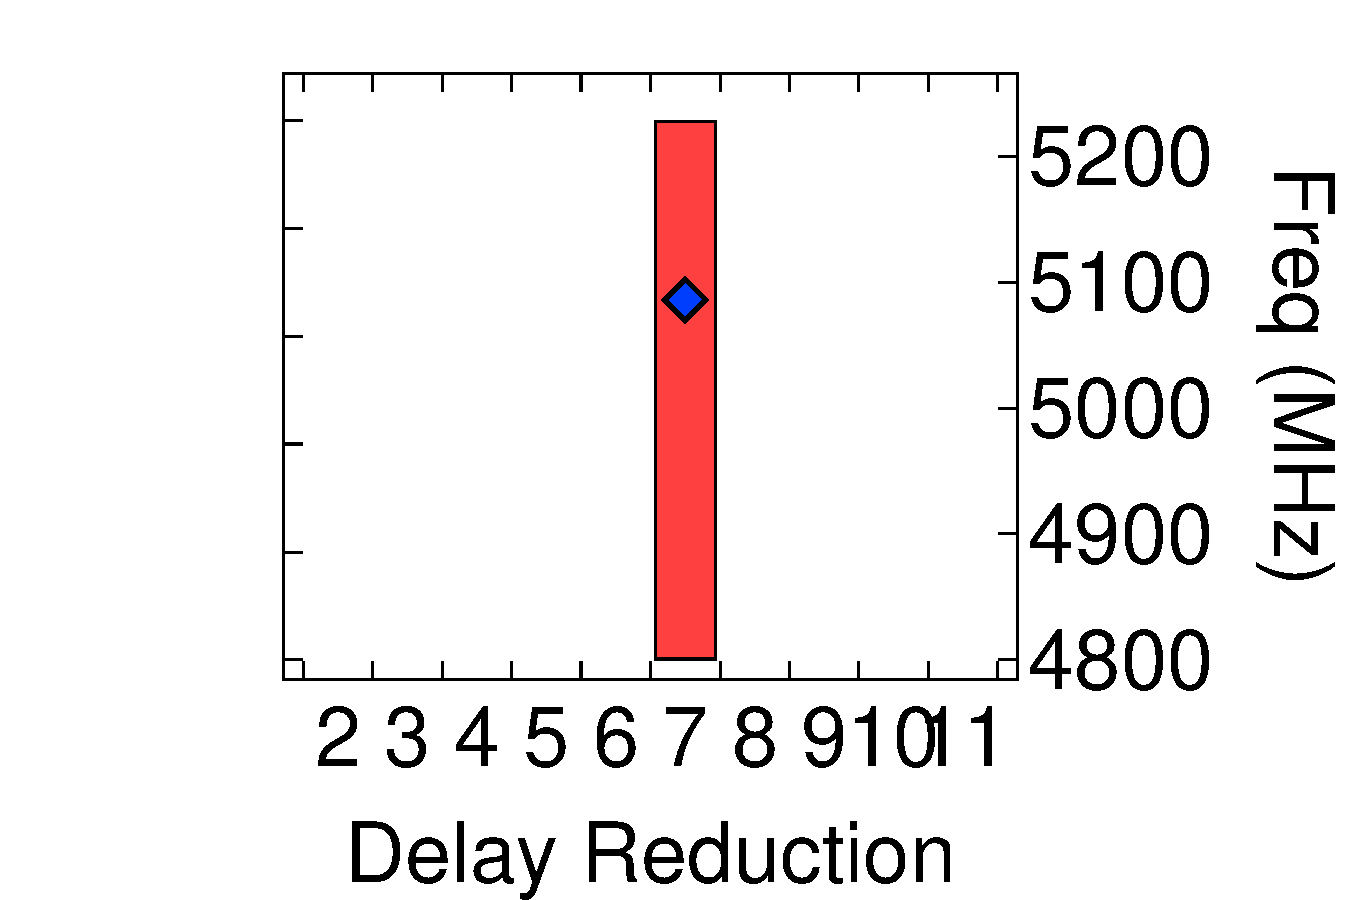
\includegraphics[trim=0 0 0 0,clip,width=.23\linewidth]{graphs/process/idle-limit-dist/idle-limit-dist-p0c5.pdf}
        \label{fig:idle_dist_p0c5} 
      }
      \hfill
      \subfloat[p0 core 6.] {
        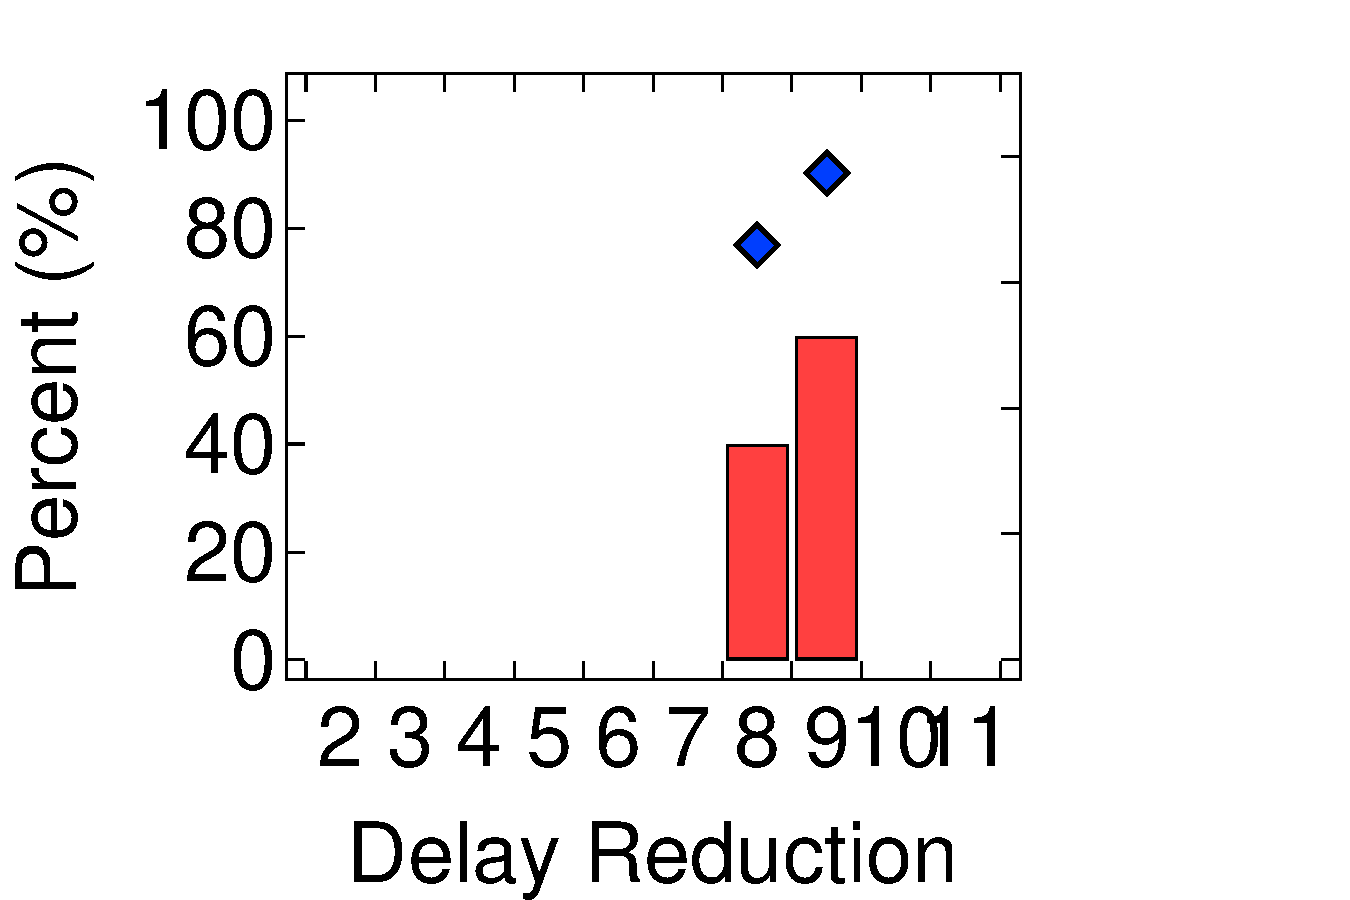
\includegraphics[trim=0 0 0 0,clip,width=.23\linewidth]{graphs/process/idle-limit-dist/idle-limit-dist-p0c6.pdf}
        \label{fig:idle_dist_p0c6} 
      }
      \hfill
      \subfloat[p0 core 7.] {
        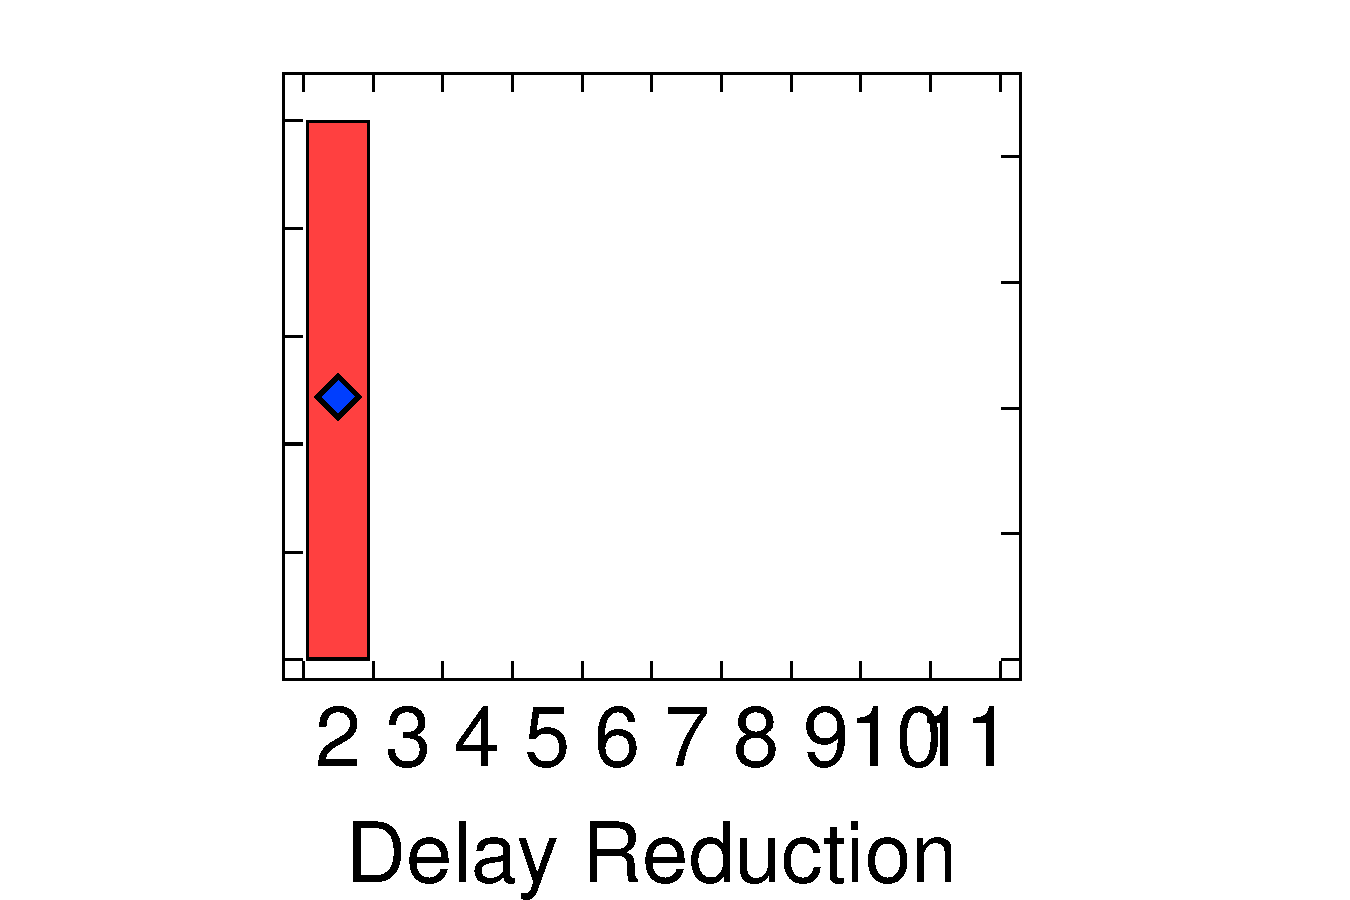
\includegraphics[trim=0 0 0 0,clip,width=.23\linewidth]{graphs/process/idle-limit-dist/idle-limit-dist-p0c7.pdf}
        \label{fig:idle_dist_p0c7} 
      }

      \subfloat[p1 core 0.] {
        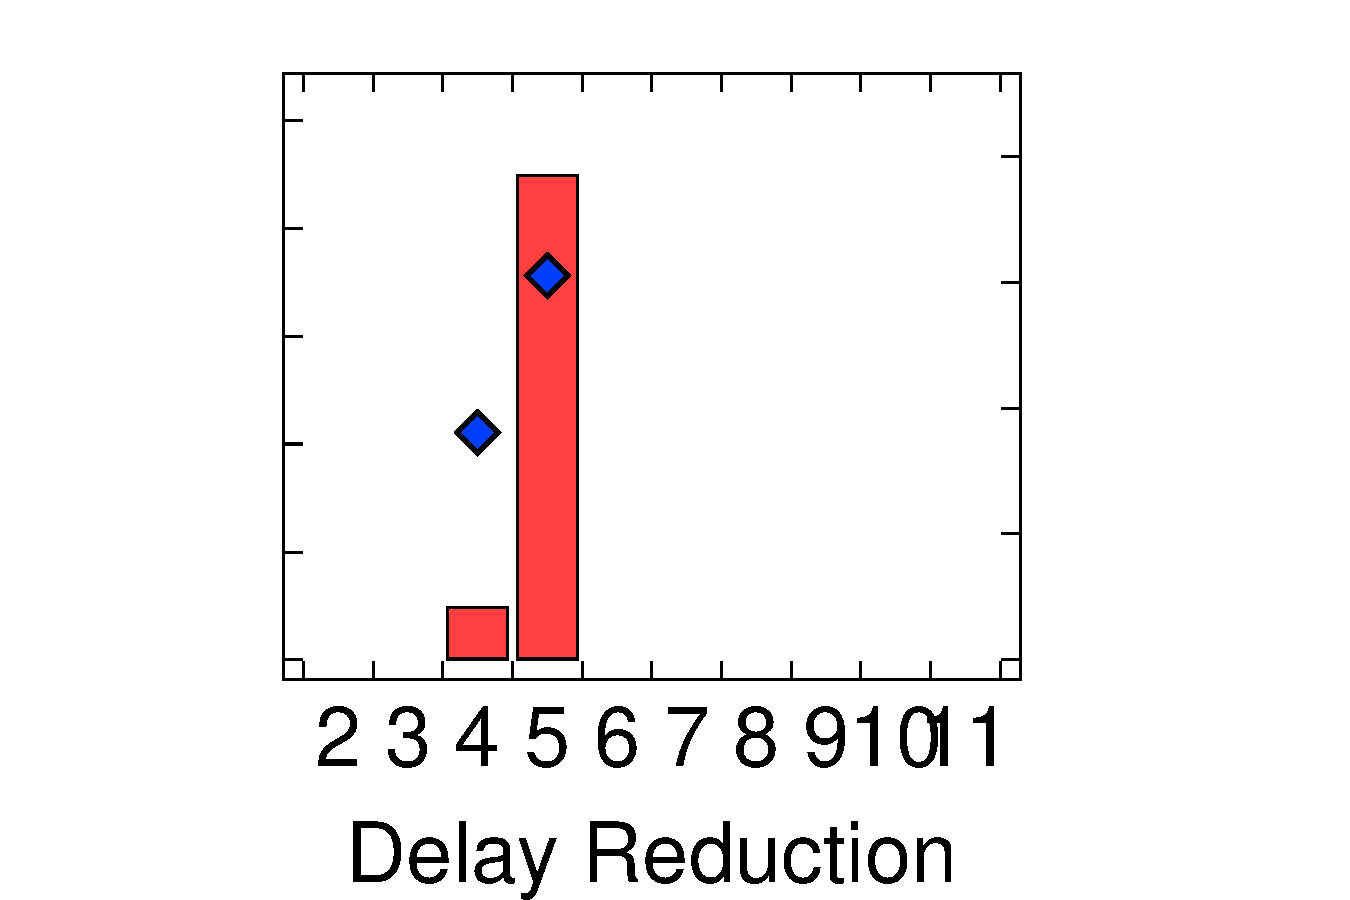
\includegraphics[trim=0 0 0 0,clip,width=.23\linewidth]{graphs/process/idle-limit-dist/idle-limit-dist-p1c0.pdf}
        \label{fig:idle_dist_p1c0}
      }
      \hfill
      \subfloat[p1 core 1.] {
        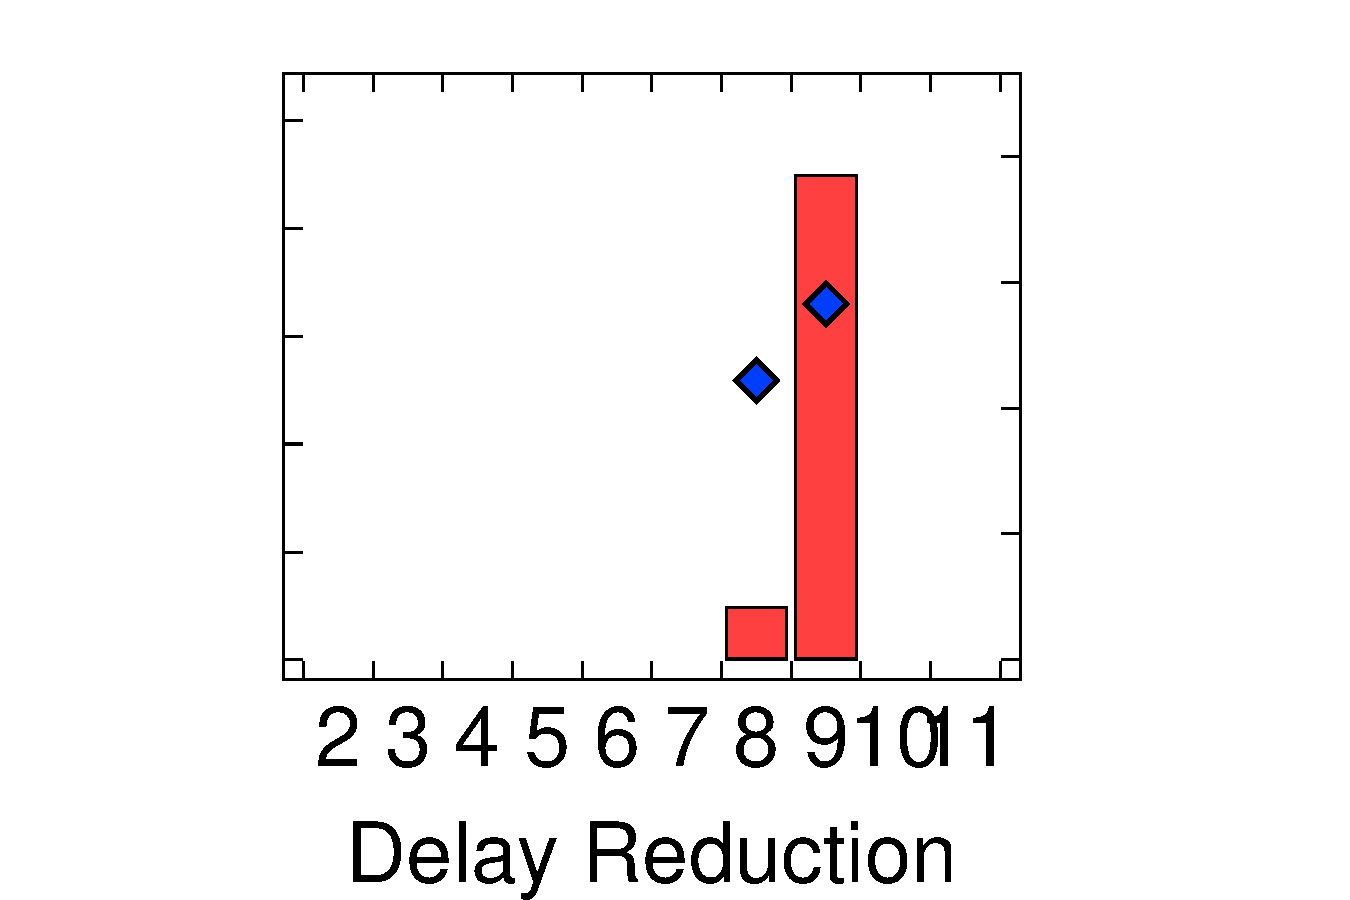
\includegraphics[trim=0 0 0 0,clip,width=.23\linewidth]{graphs/process/idle-limit-dist/idle-limit-dist-p1c1.pdf}
        \label{fig:idle_dist_p1c1} 
      }
      \hfill
      \subfloat[p1 Core 2.] {
        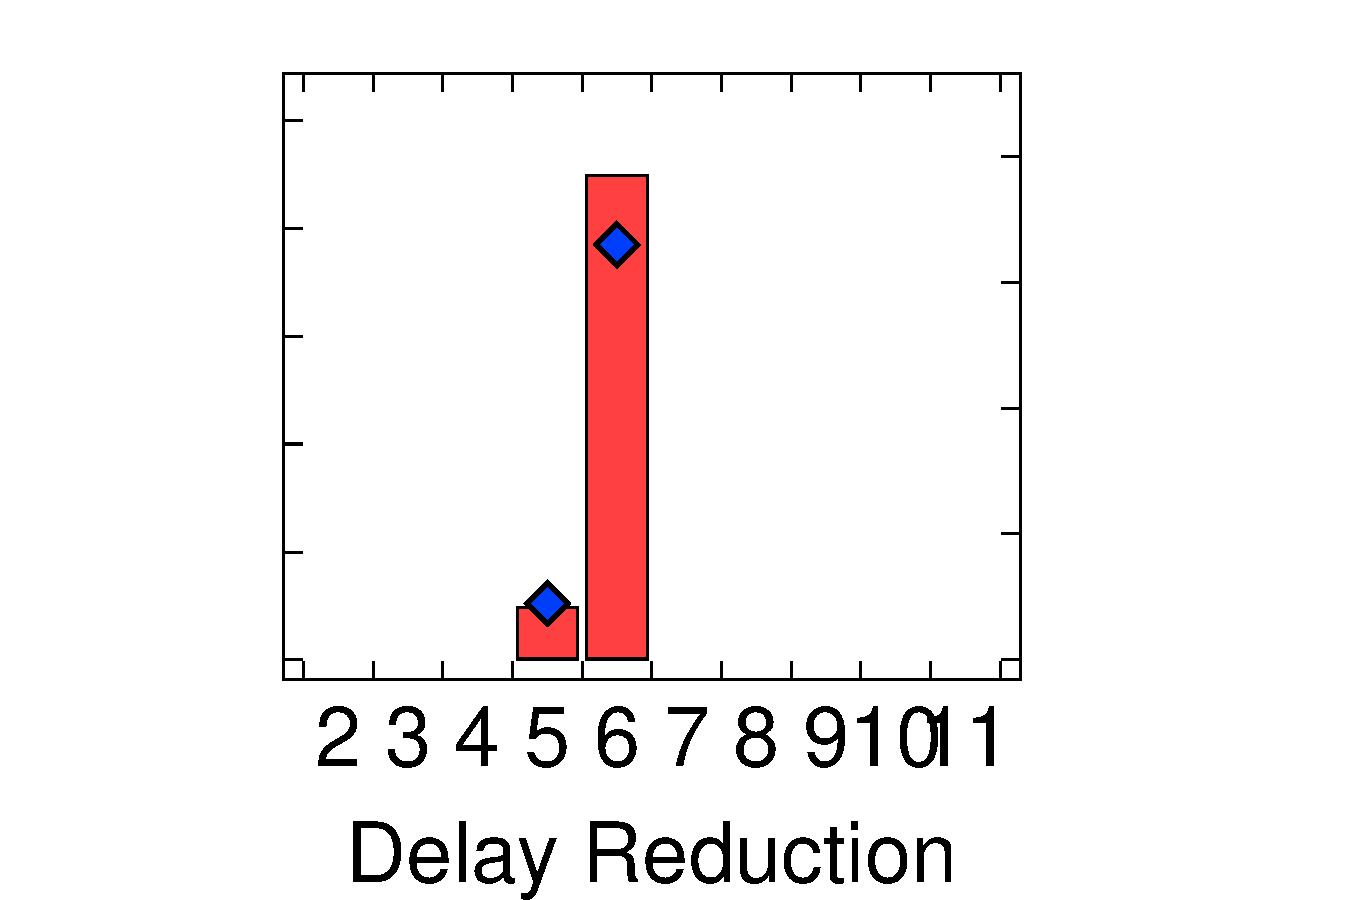
\includegraphics[trim=0 0 0 0,clip,width=.23\linewidth]{graphs/process/idle-limit-dist/idle-limit-dist-p1c2.pdf}
        \label{fig:idle_dist_p1c2} 
      }
      \hfill
      \subfloat[p1 Core 3.] {
        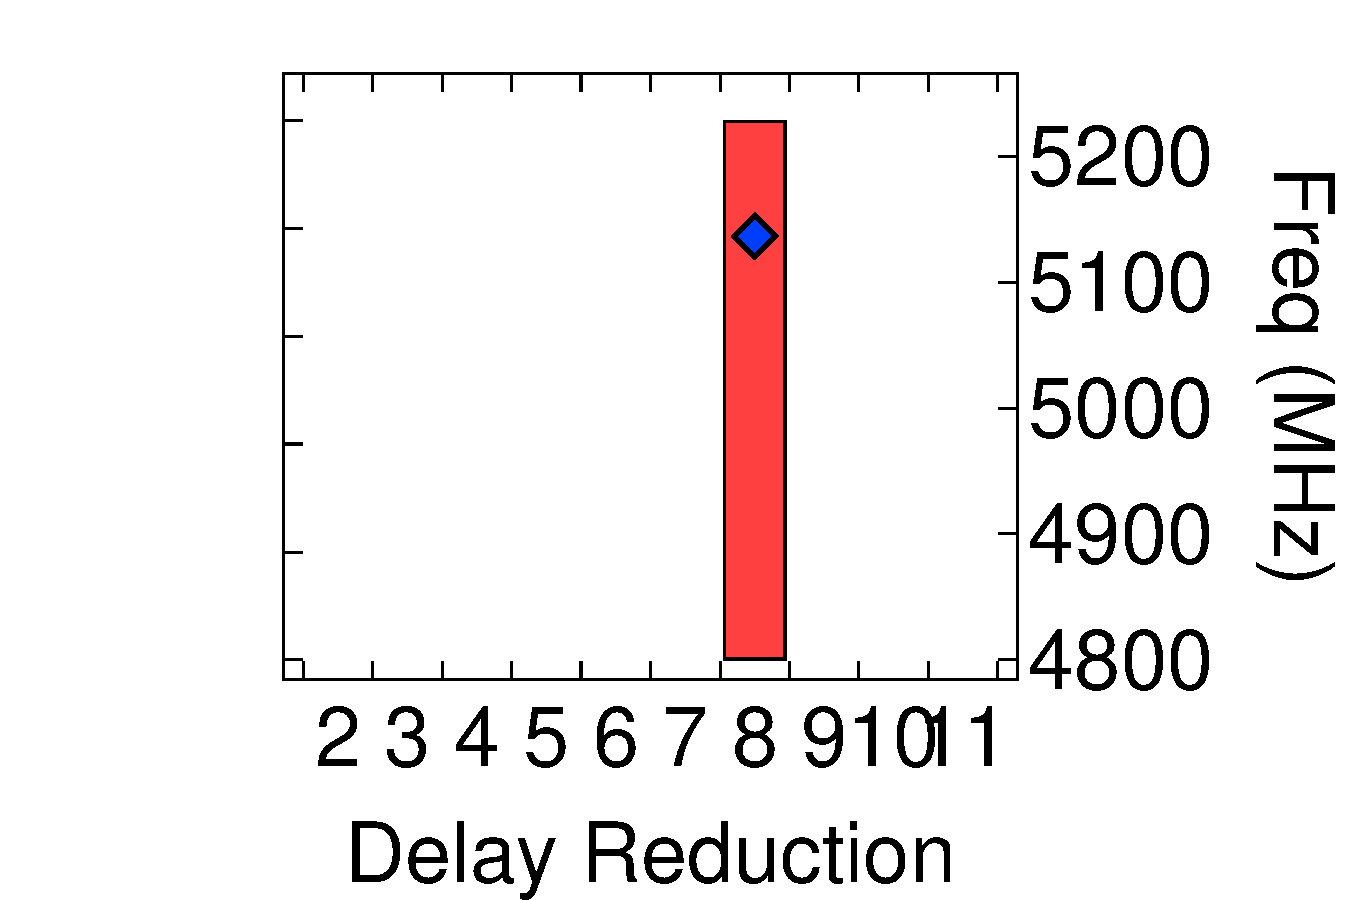
\includegraphics[trim=0 0 0 0,clip,width=.23\linewidth]{graphs/process/idle-limit-dist/idle-limit-dist-p1c3.pdf}
        \label{fig:idle_dist_p1c3} 
      }

      \subfloat[p1 Core 4.] {
        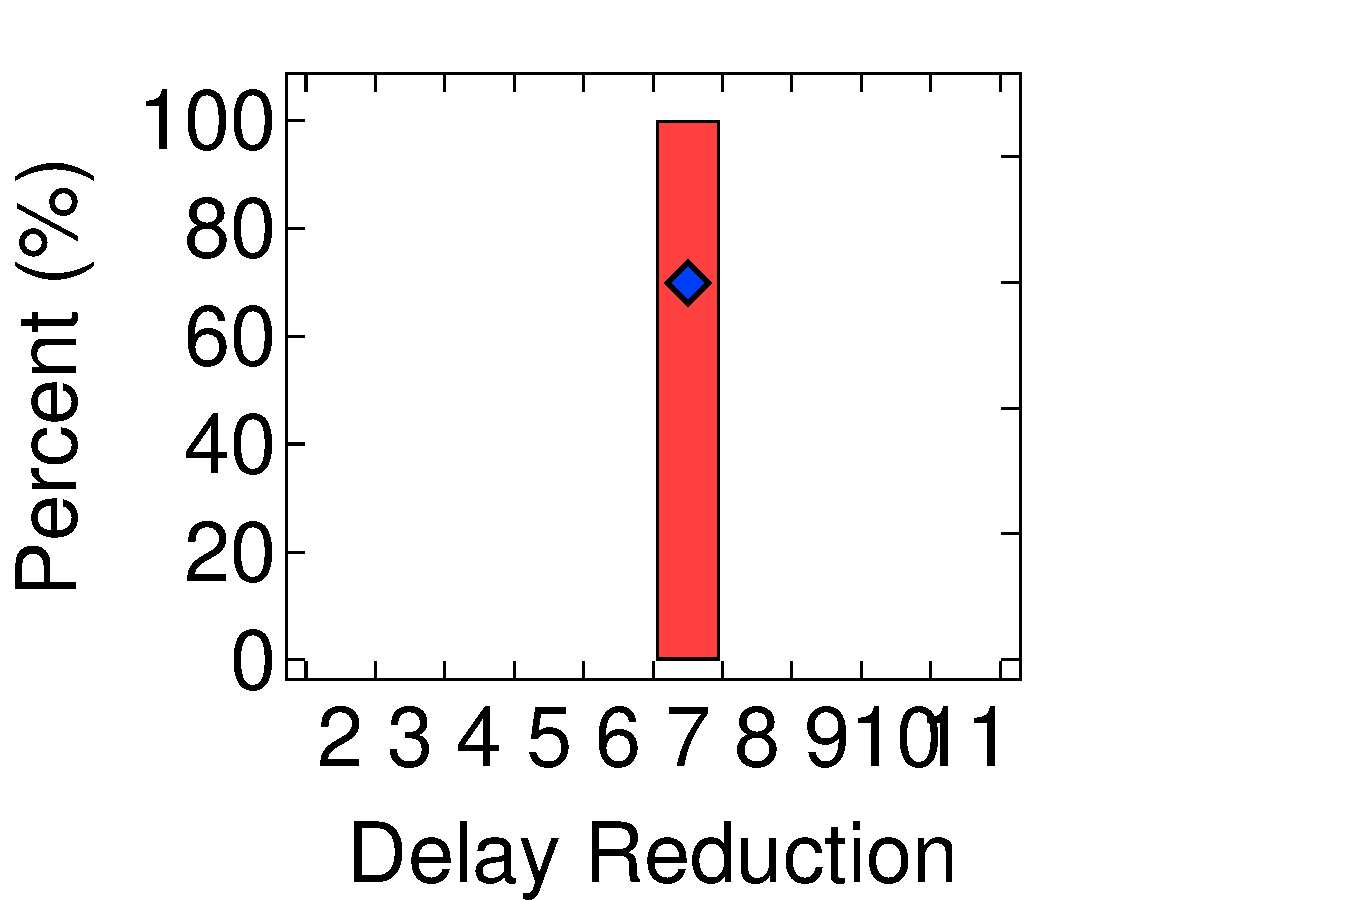
\includegraphics[trim=0 0 0 0,clip,width=.23\linewidth]{graphs/process/idle-limit-dist/idle-limit-dist-p1c4.pdf}
        \label{fig:idle_dist_p1c4} 
      }
      \hfill
      \subfloat[p1 Core 5.] {
        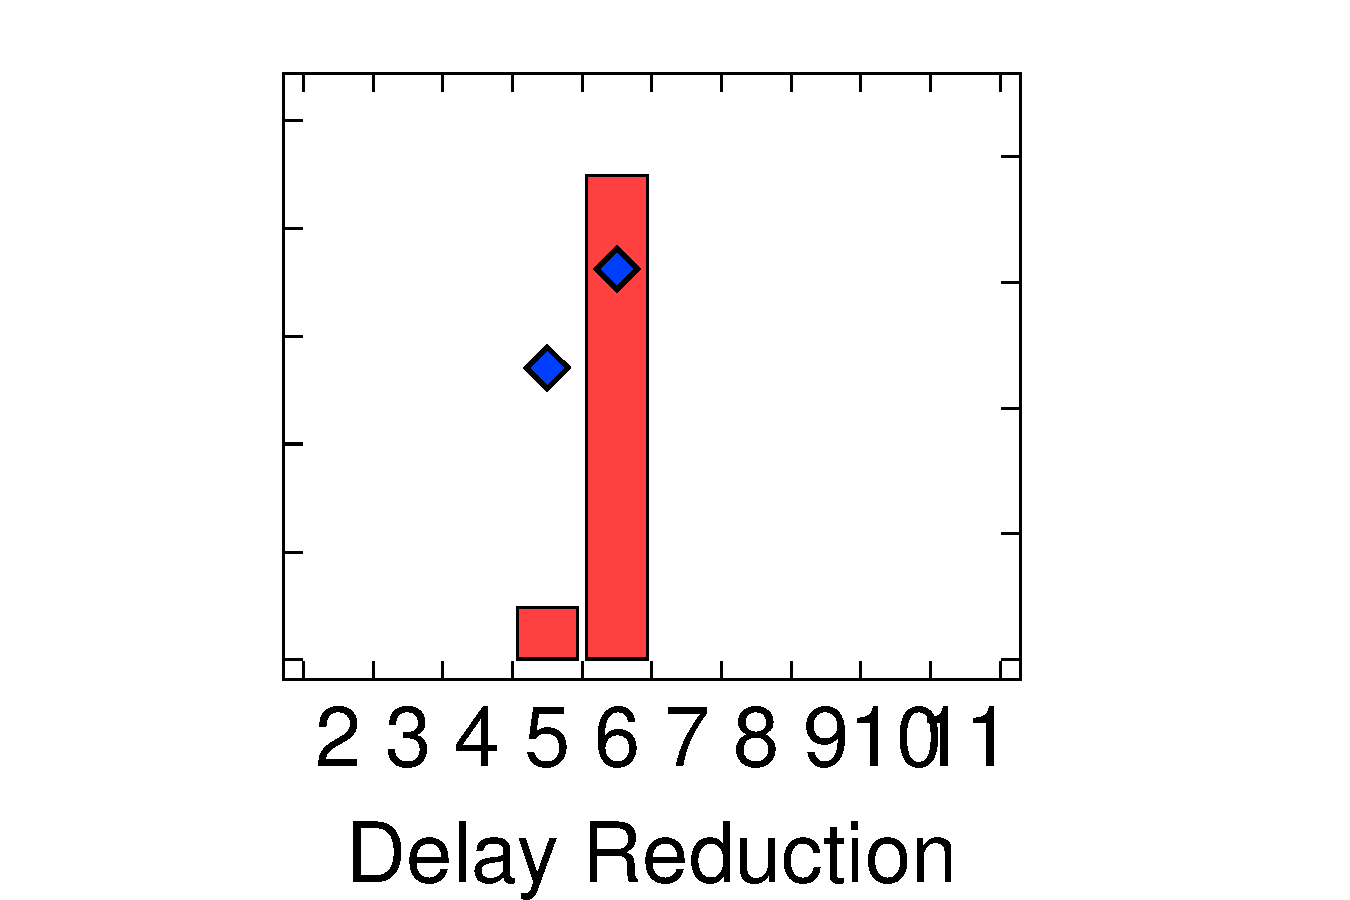
\includegraphics[trim=0 0 0 0,clip,width=.23\linewidth]{graphs/process/idle-limit-dist/idle-limit-dist-p1c5.pdf}
        \label{fig:idle_dist_p1c5} 
      }
      \hfill
      \subfloat[p1 Core 6.] {
        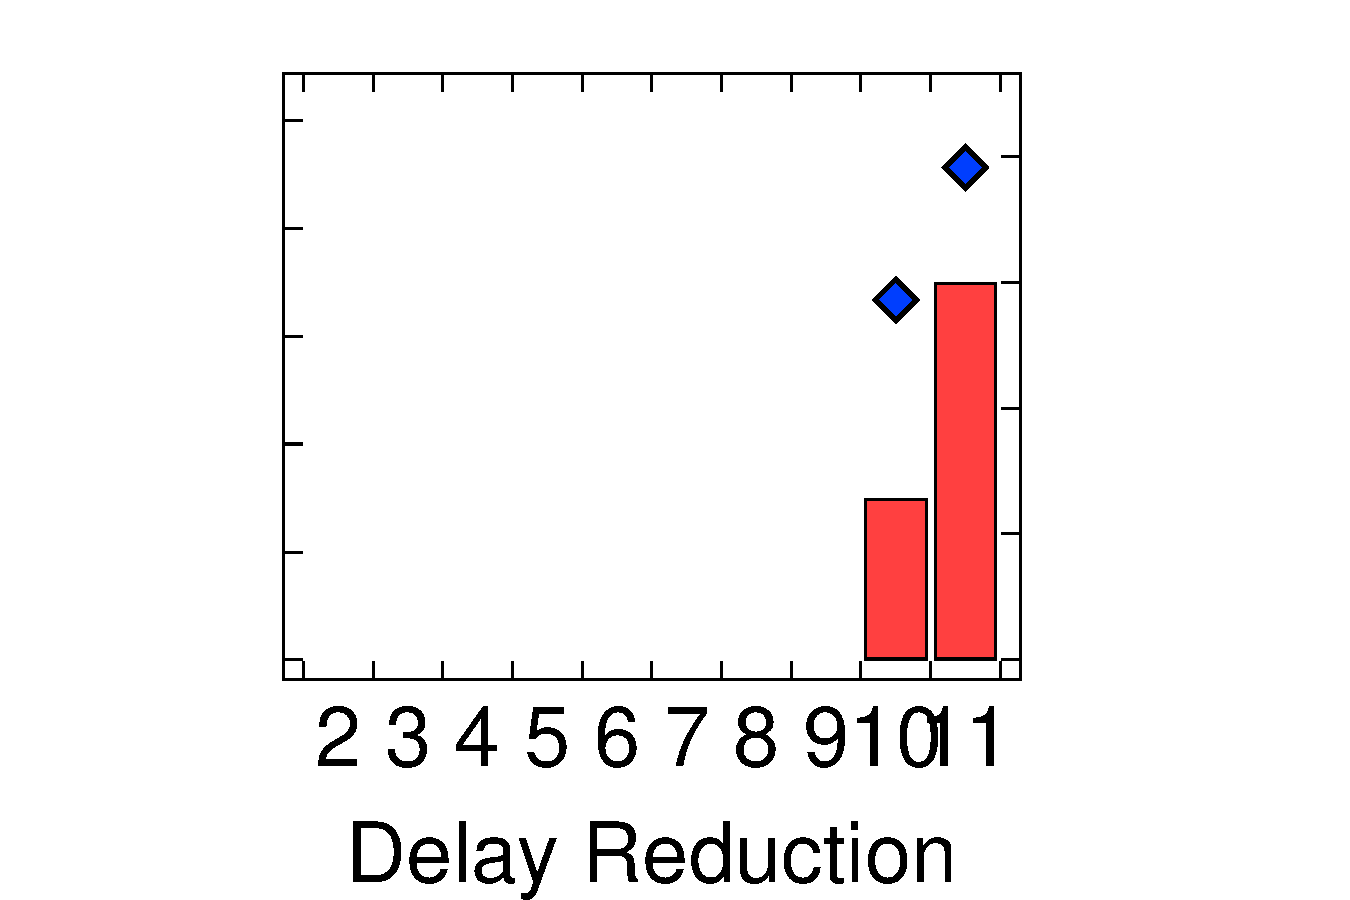
\includegraphics[trim=0 0 0 0,clip,width=.23\linewidth]{graphs/process/idle-limit-dist/idle-limit-dist-p1c6.pdf}
        \label{fig:idle_dist_p1c6} 
      }
      \hfill
      \subfloat[p1 Core 7.] {
        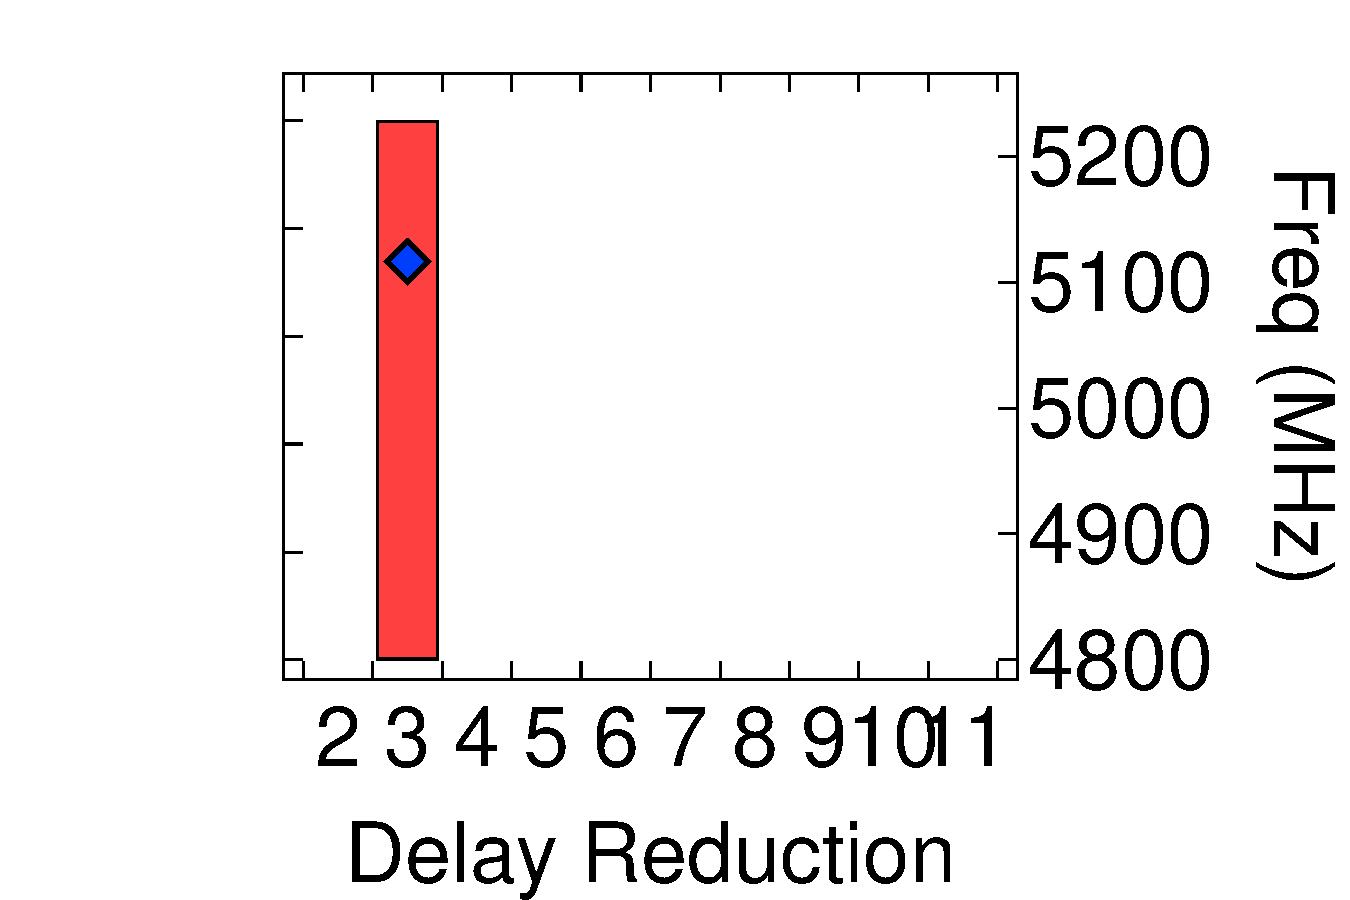
\includegraphics[trim=0 0 0 0,clip,width=.23\linewidth]{graphs/process/idle-limit-dist/idle-limit-dist-p1c7.pdf}
        \label{fig:idle_dist_p1c7} 
      }
    %TODO: this graph can be cut in half (deleting p1's data) to shrink paper length
    \caption{The limit configuration of each POWER7+ core (i.e., the most aggressive reduction of CPM's inserted delay from its default setting, beyond which ATM operation can cause system failure under idle condition) distributes over a narrow range (red bar, left y axis). The operating frequency at each core's limit delay config is over 4800~MHz, more than 15\% higher than static margin's 4200~MHz level (blue mark, right y axis).}
    
    \label{fig:idle-limit-dist} 
\end{figure*}

% \begin{figure*}[t]
%      \subfloat[p0 core 0.] {
%        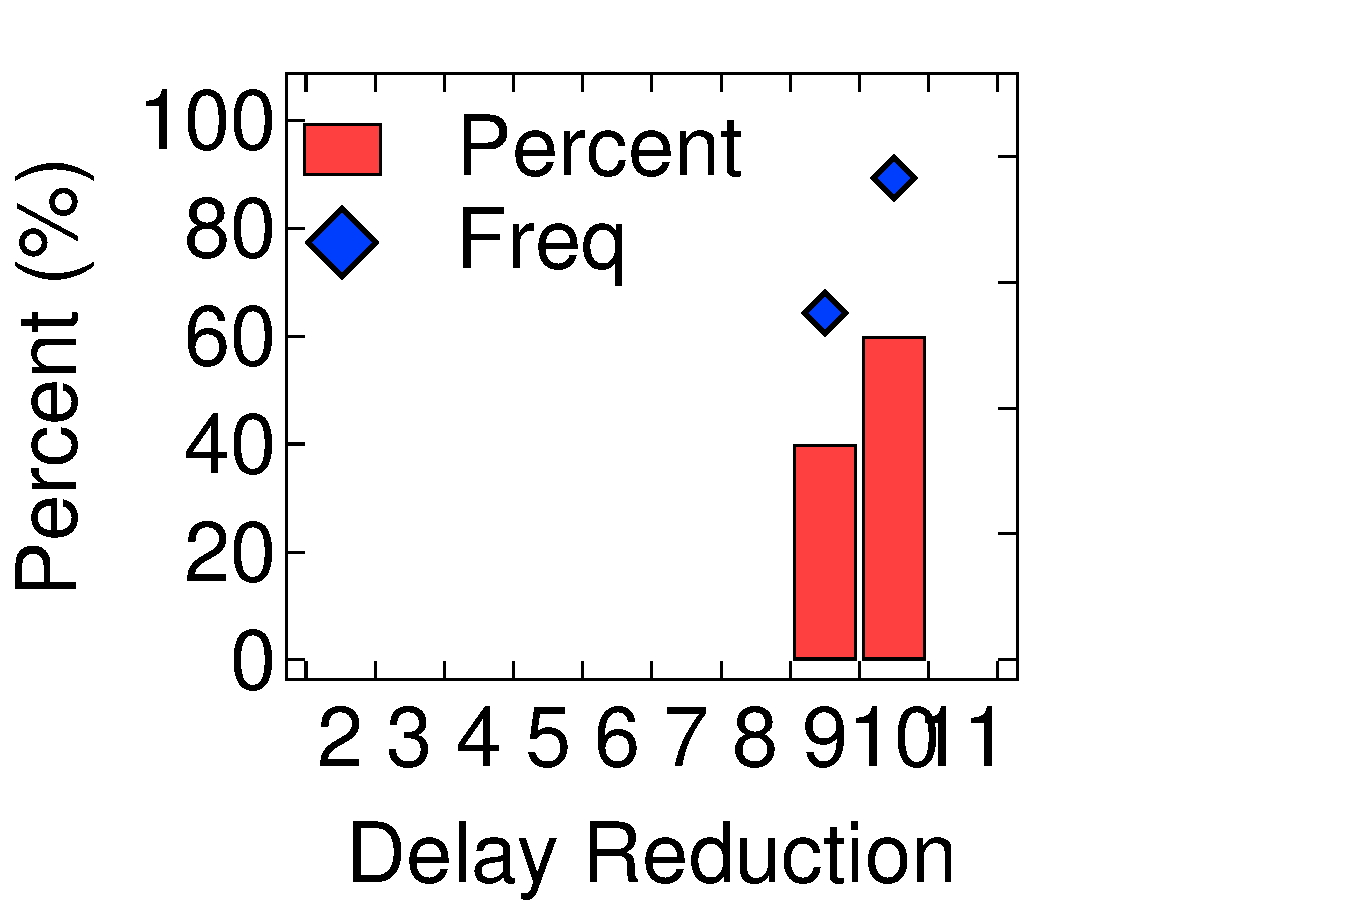
\includegraphics[trim=0 0 140 0,clip,width=.183\linewidth]{graphs/process/idle-limit-dist/idle-limit-dist-p0c0.pdf}
%        \label{fig:idle_dist_p0c0}
%      }
%      \hfill
%      \subfloat[p0 core 1.] {
%        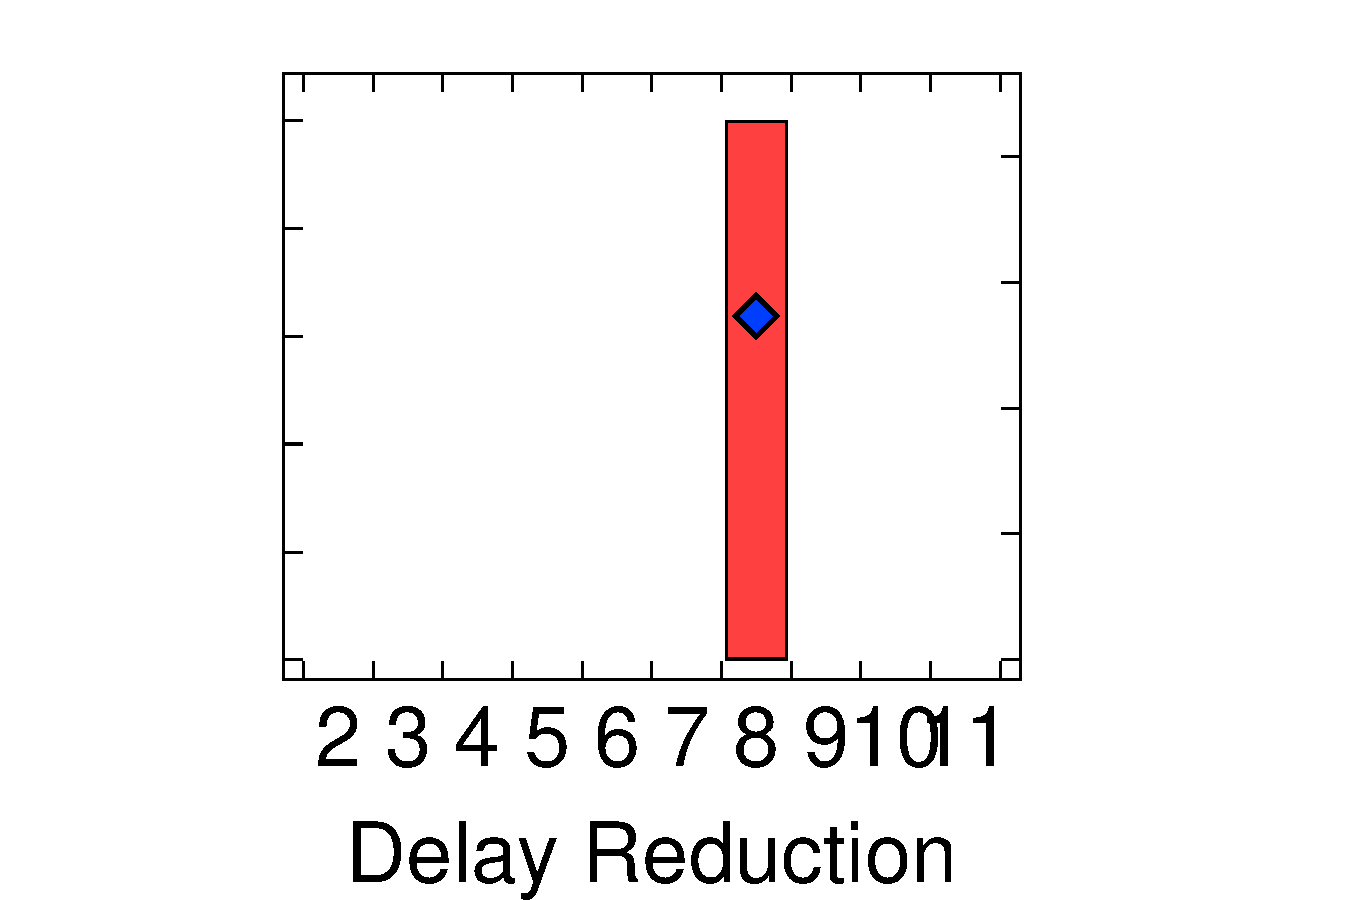
\includegraphics[trim=135 0 140 0,clip,width=.134\linewidth]{graphs/process/idle-limit-dist/idle-limit-dist-p0c1.pdf}
%        \label{fig:idle_dist_p0c1} 
%      }
%      \hfill
%      \subfloat[p0 core 2.] {
%        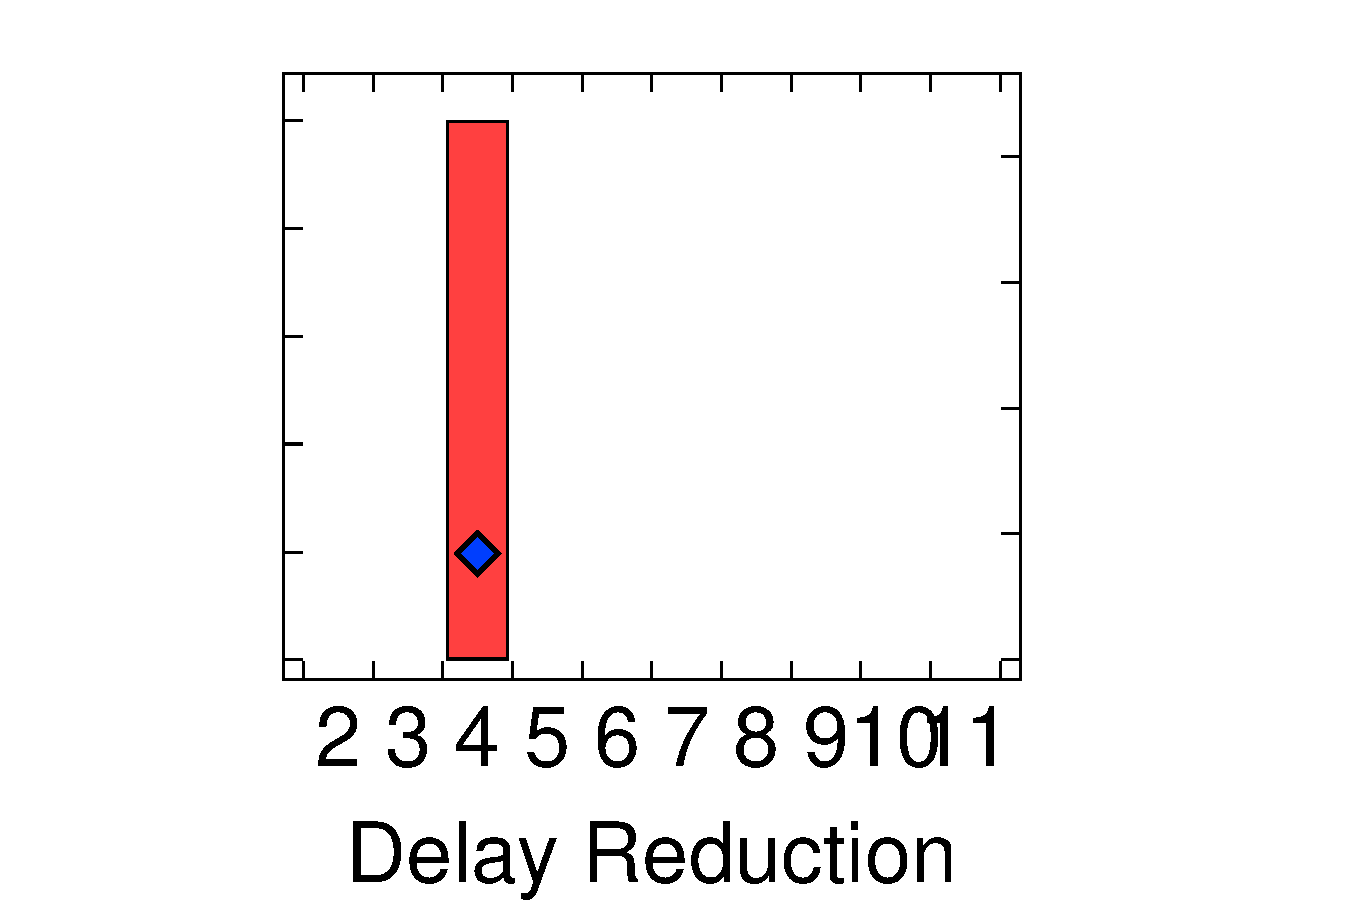
\includegraphics[trim=135 0 140 0,clip,width=.134\linewidth]{graphs/process/idle-limit-dist/idle-limit-dist-p0c2.pdf}
%        \label{fig:idle_dist_p0c2} 
%      }
%      \hfill
%      \subfloat[p0 core 3.] {
%        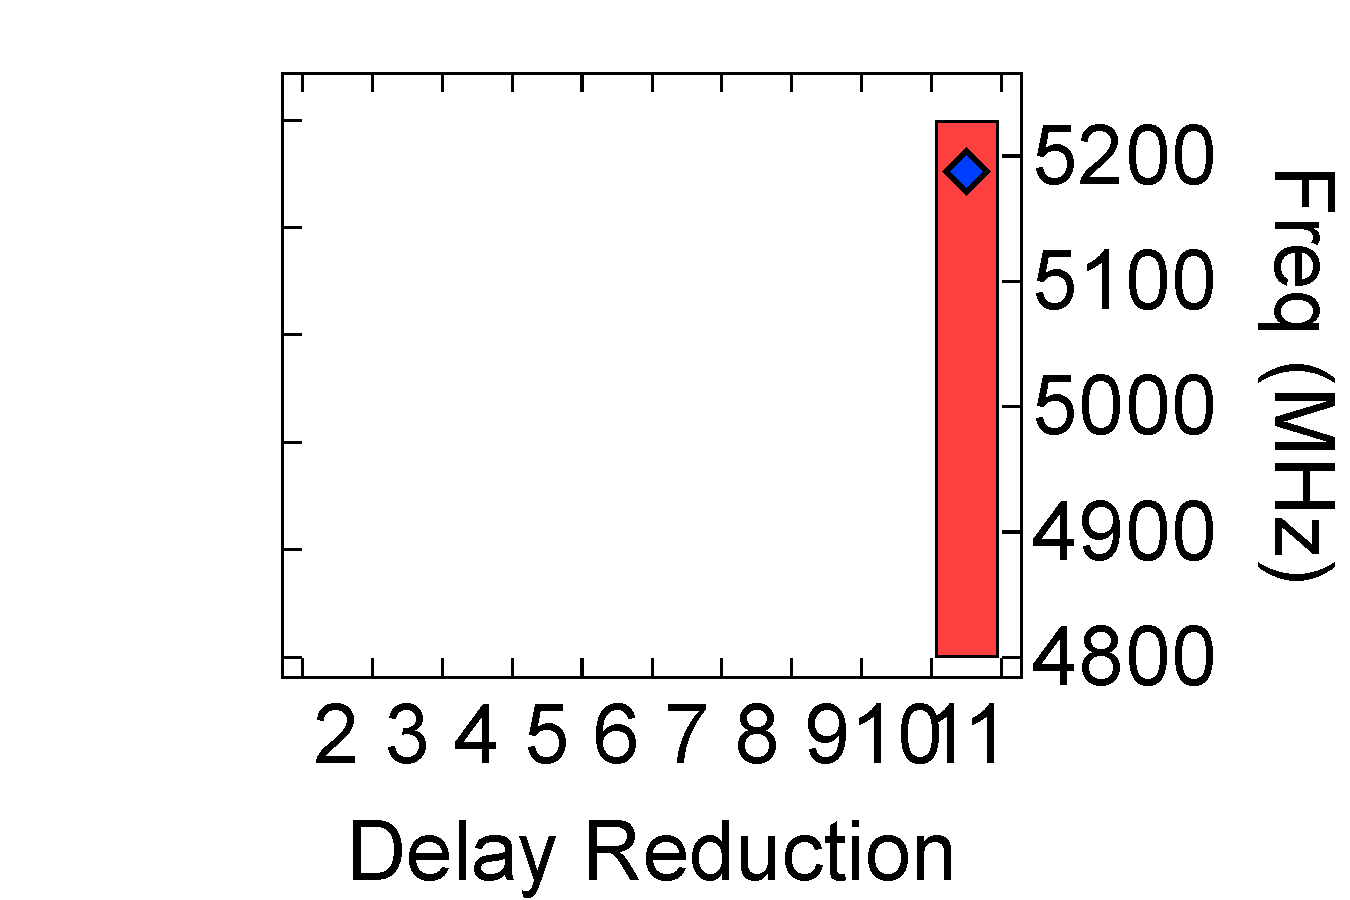
\includegraphics[trim=135 0 140 0,clip,width=.134\linewidth]{graphs/process/idle-limit-dist/idle-limit-dist-p0c3.pdf}
%        \label{fig:idle_dist_p0c3} 
%      }

%      \subfloat[p0 core 4.] {
%        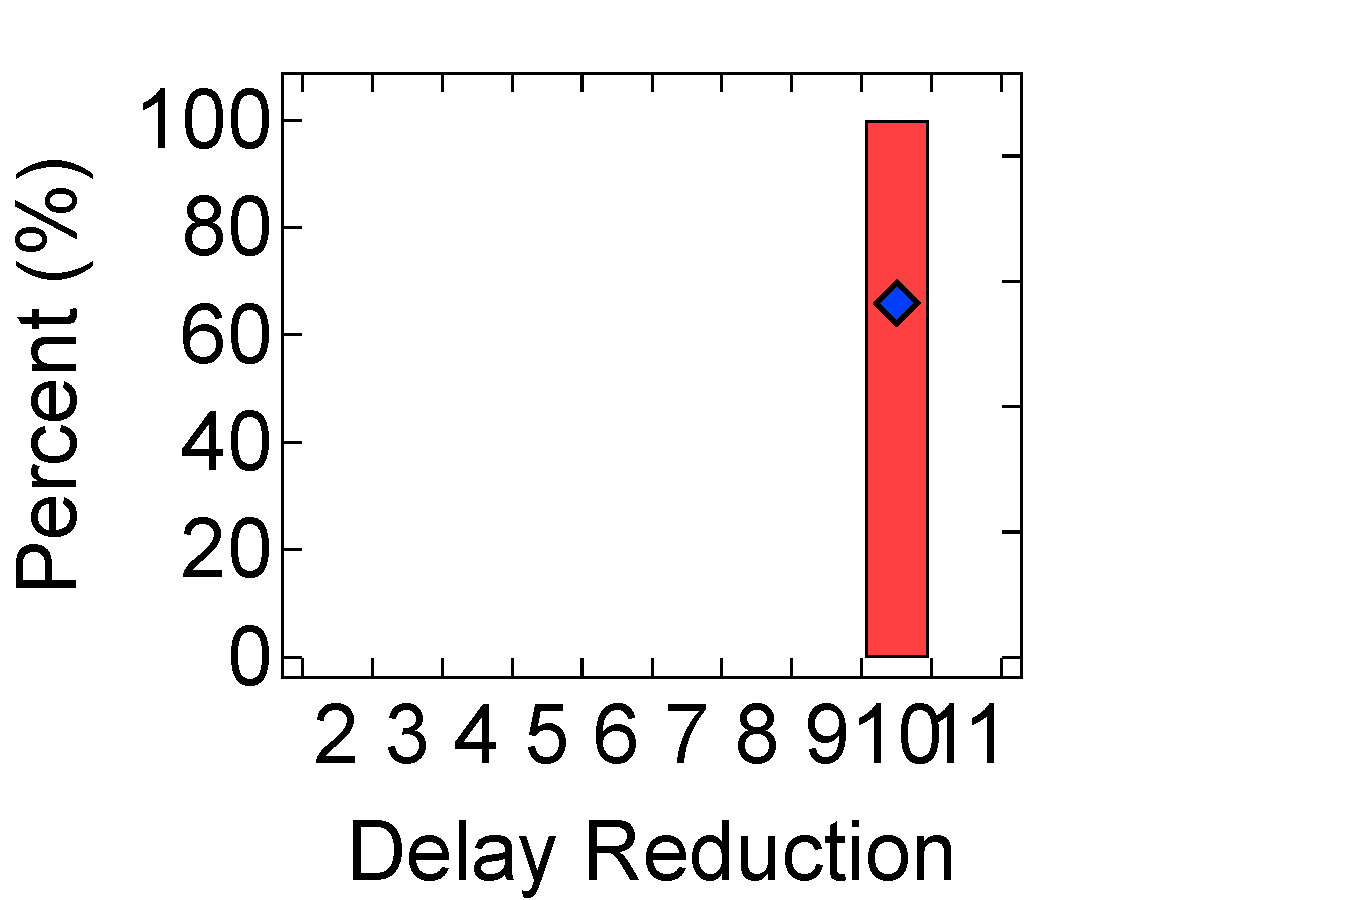
\includegraphics[trim=135 0 140 0,clip,width=.134\linewidth]{graphs/process/idle-limit-dist/idle-limit-dist-p0c4.pdf}
%        \label{fig:idle_dist_p0c4} 
%      }
%      \hfill
%      \subfloat[p0 core 5.] {
%        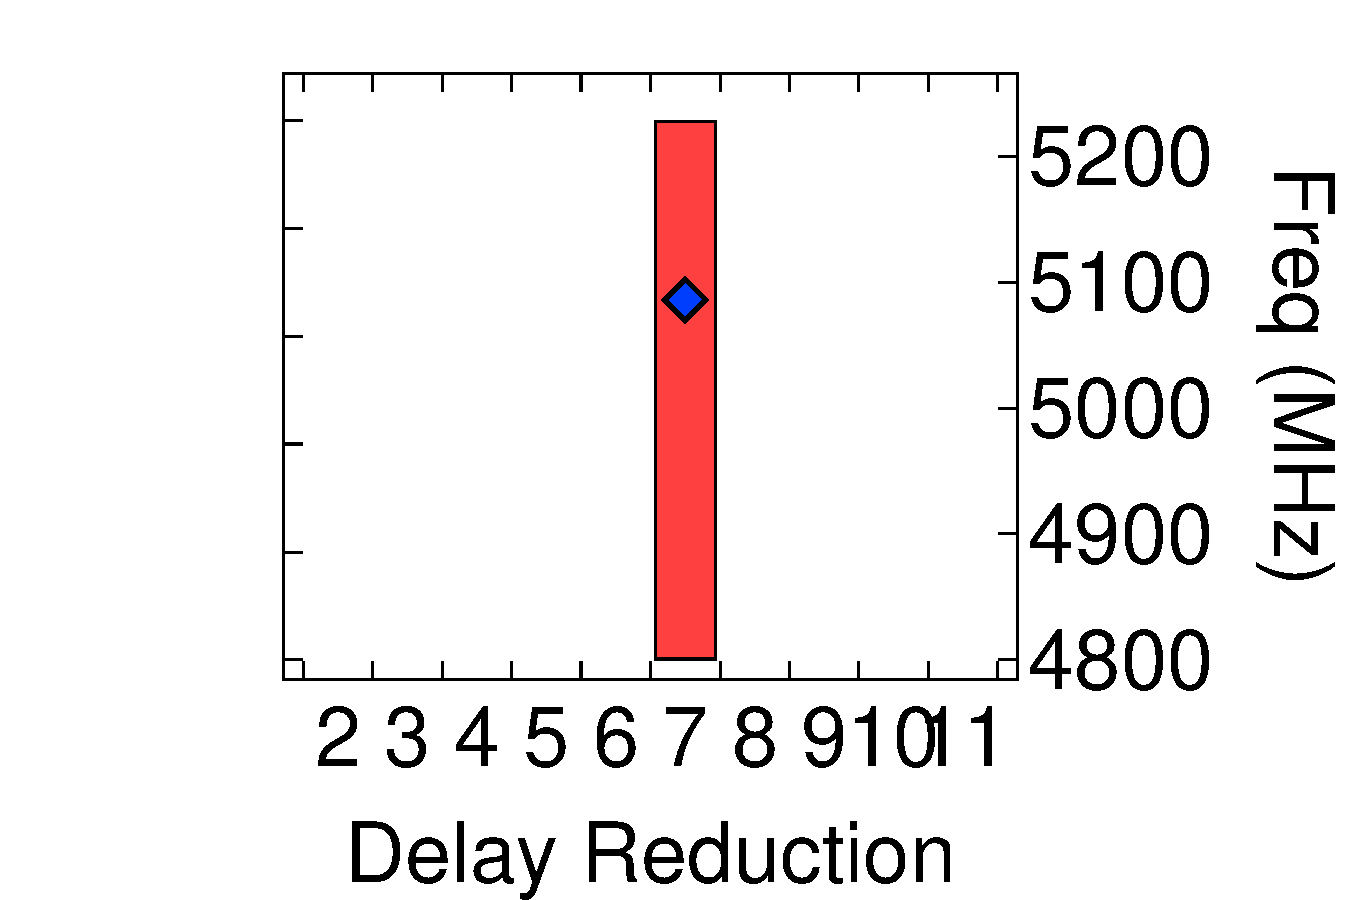
\includegraphics[trim=135 0 0 0,clip,width=.185\linewidth]{graphs/process/idle-limit-dist/idle-limit-dist-p0c5.pdf}
%        \label{fig:idle_dist_p0c5} 
%      }
%      \hfill
%      \subfloat[p0 core 6.] {
%        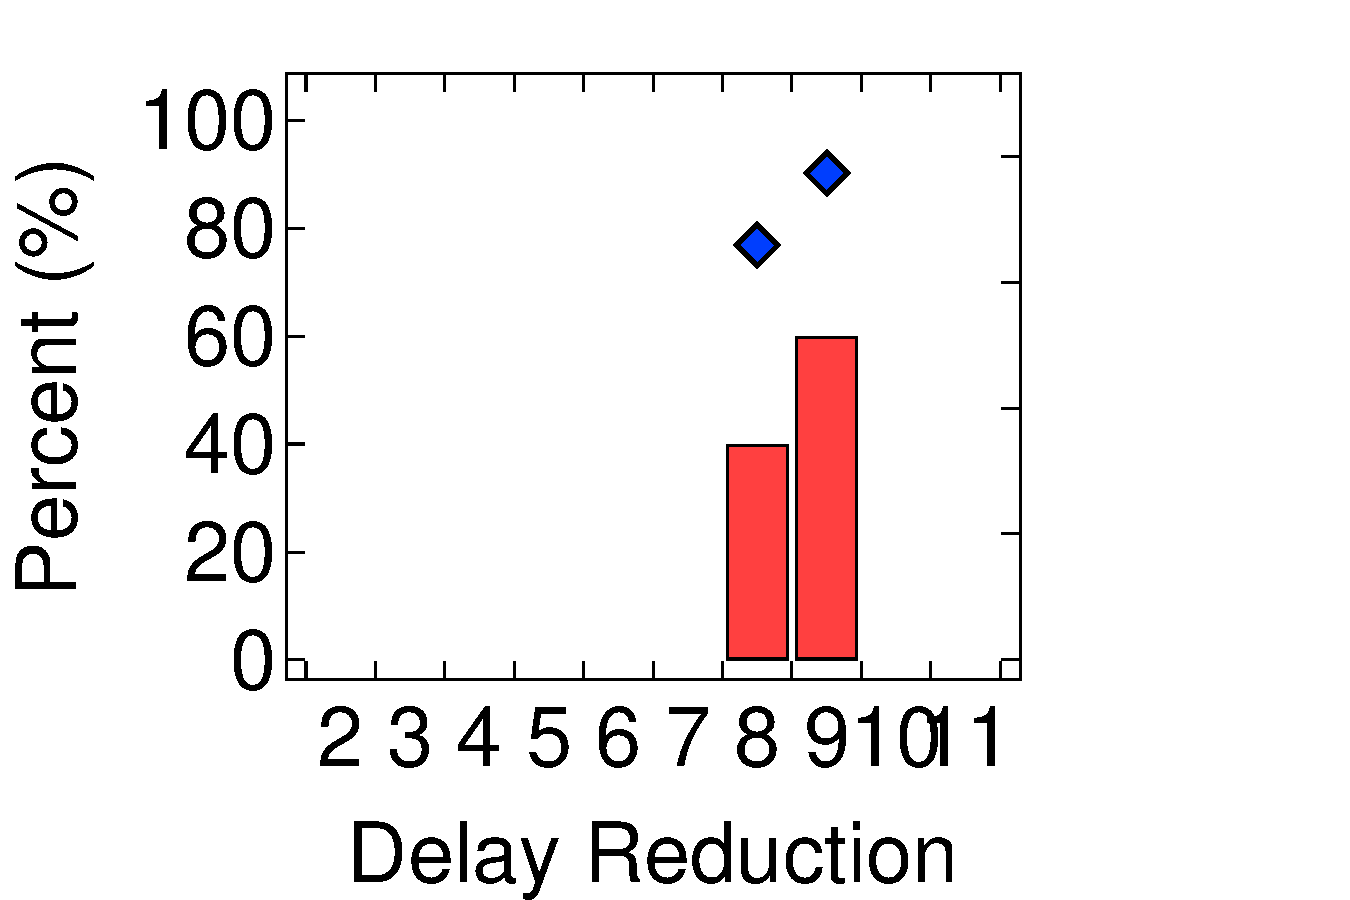
\includegraphics[trim=0 0 140 0,clip,width=.183\linewidth]{graphs/process/idle-limit-dist/idle-limit-dist-p0c6.pdf}
%        \label{fig:idle_dist_p0c6} 
%      }
%      \hfill
%      \subfloat[p0 core 7.] {
%        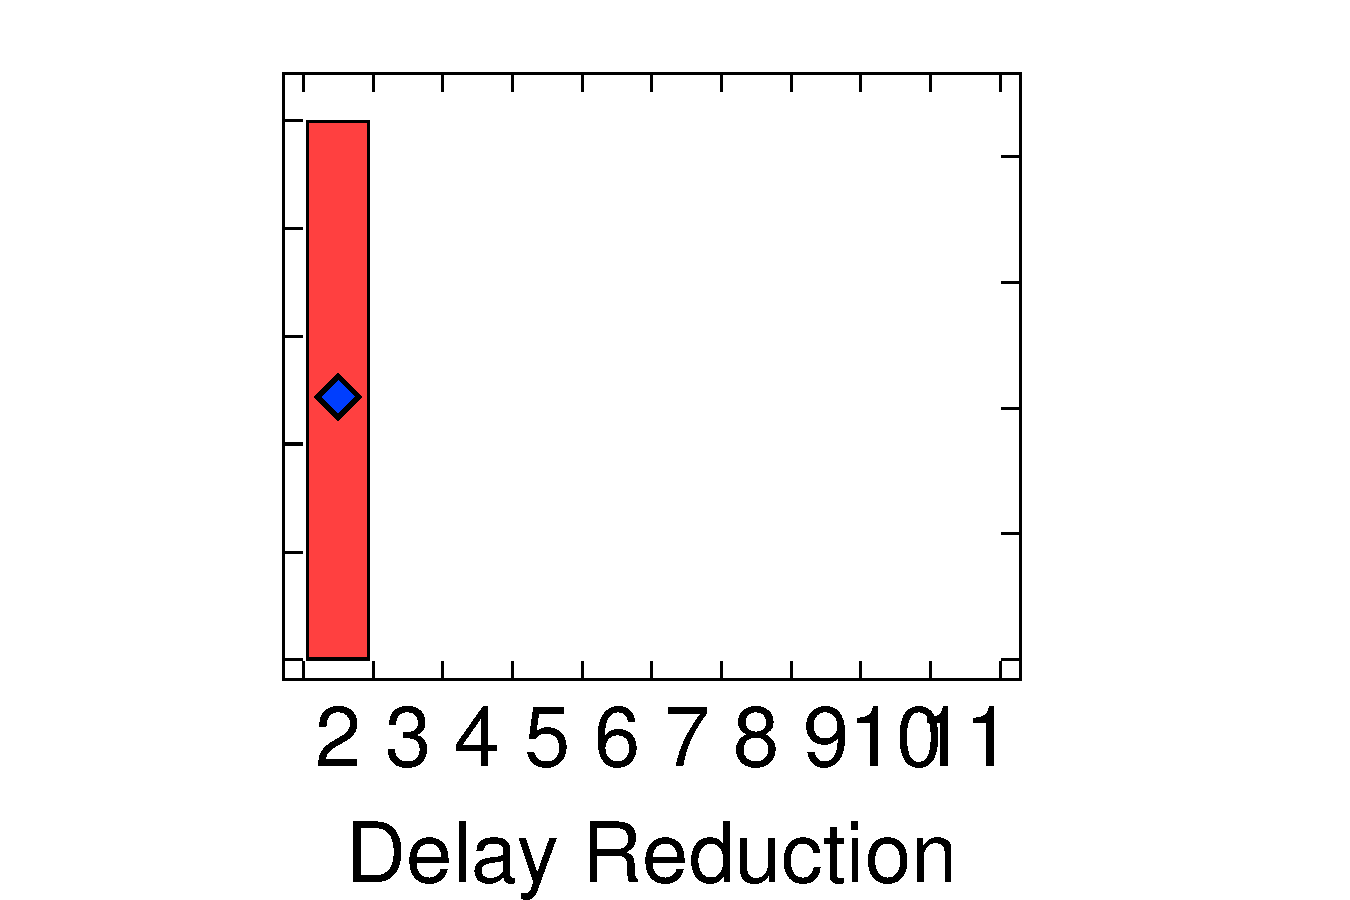
\includegraphics[trim=135 0 140 0,clip,width=.134\linewidth]{graphs/process/idle-limit-dist/idle-limit-dist-p0c7.pdf}
%        \label{fig:idle_dist_p0c7} 
%      }
%      %\hfill
%      \subfloat[p1 core 0.] {
%        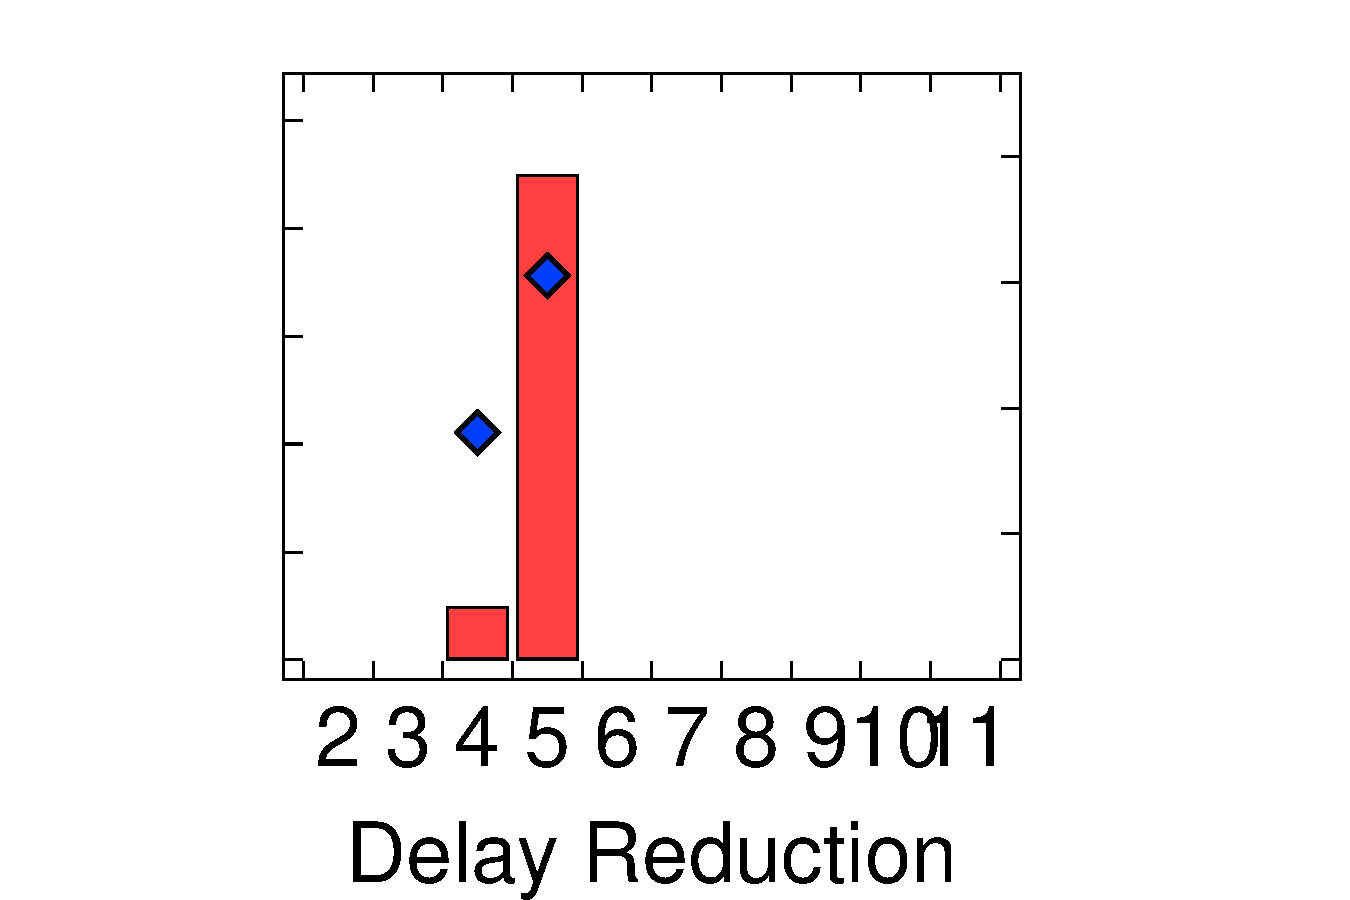
\includegraphics[trim=135 0 140 0,clip,width=.134\linewidth]{graphs/process/idle-limit-dist/idle-limit-dist-p1c0.pdf}
%        \label{fig:idle_dist_p1c0}
%      }
%      %\hfill
%      \subfloat[p1 core 1.] {
%        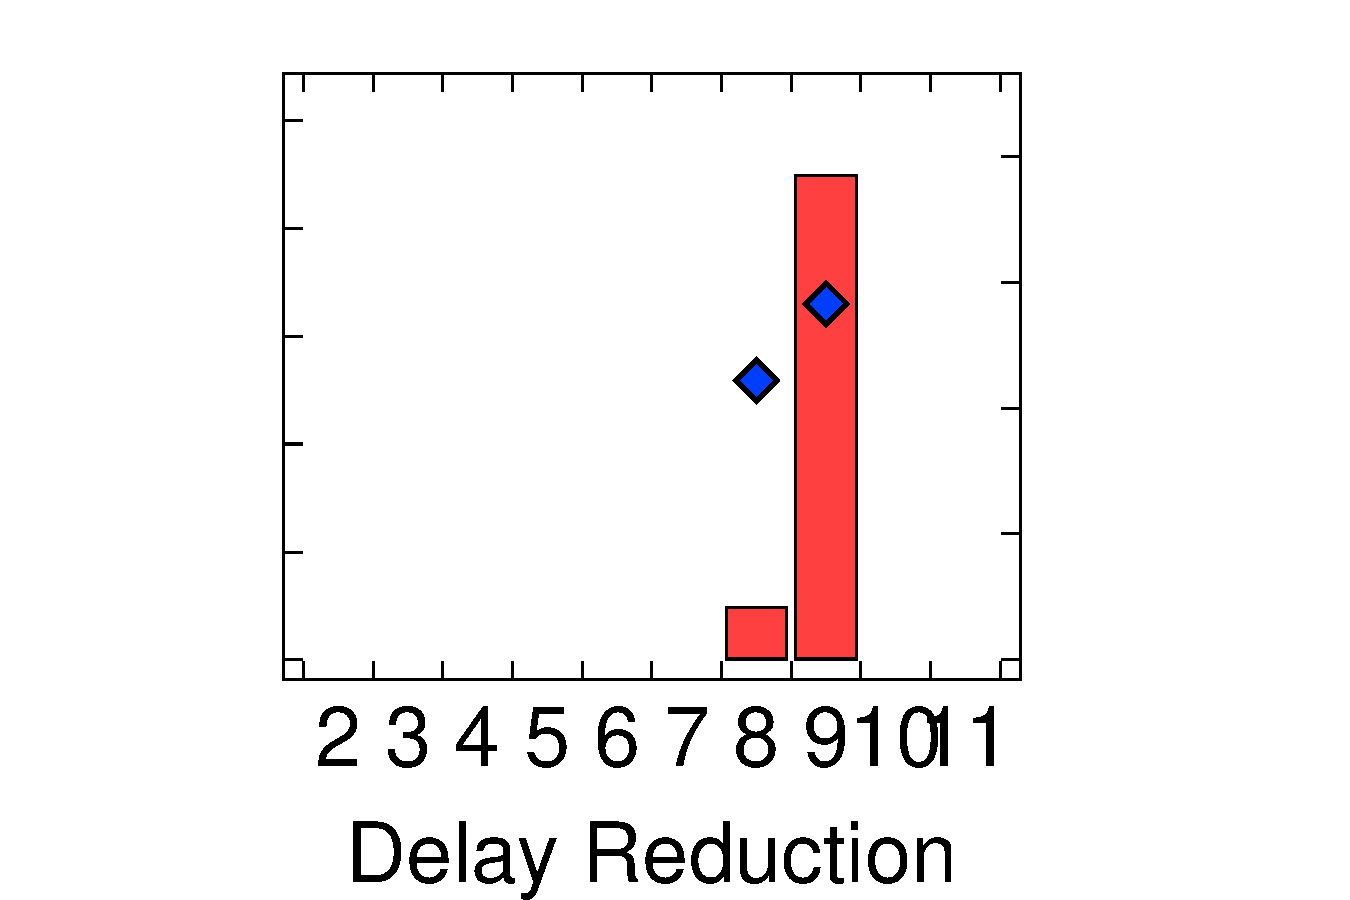
\includegraphics[trim=135 0 140 0,clip,width=.134\linewidth]{graphs/process/idle-limit-dist/idle-limit-dist-p1c1.pdf}
%        \label{fig:idle_dist_p1c1} 
%      }
%      %\hfill
%      \subfloat[p1 Core 2.] {
%        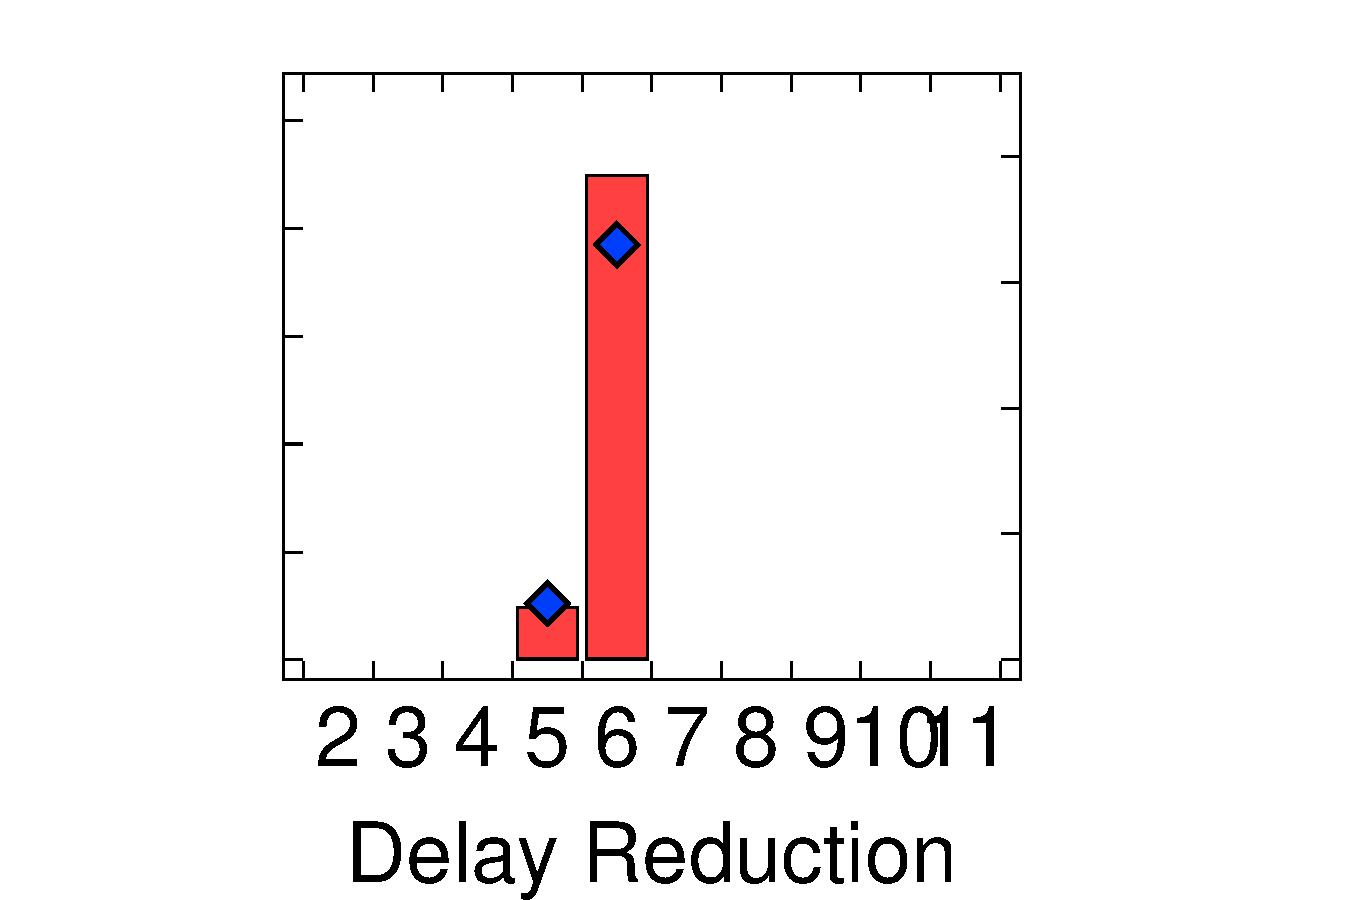
\includegraphics[trim=135 0 140 0,clip,width=.134\linewidth]{graphs/process/idle-limit-dist/idle-limit-dist-p1c2.pdf}
%        \label{fig:idle_dist_p1c2} 
%      }
%      %\hfill
%      \subfloat[p1 Core 3.] {
%        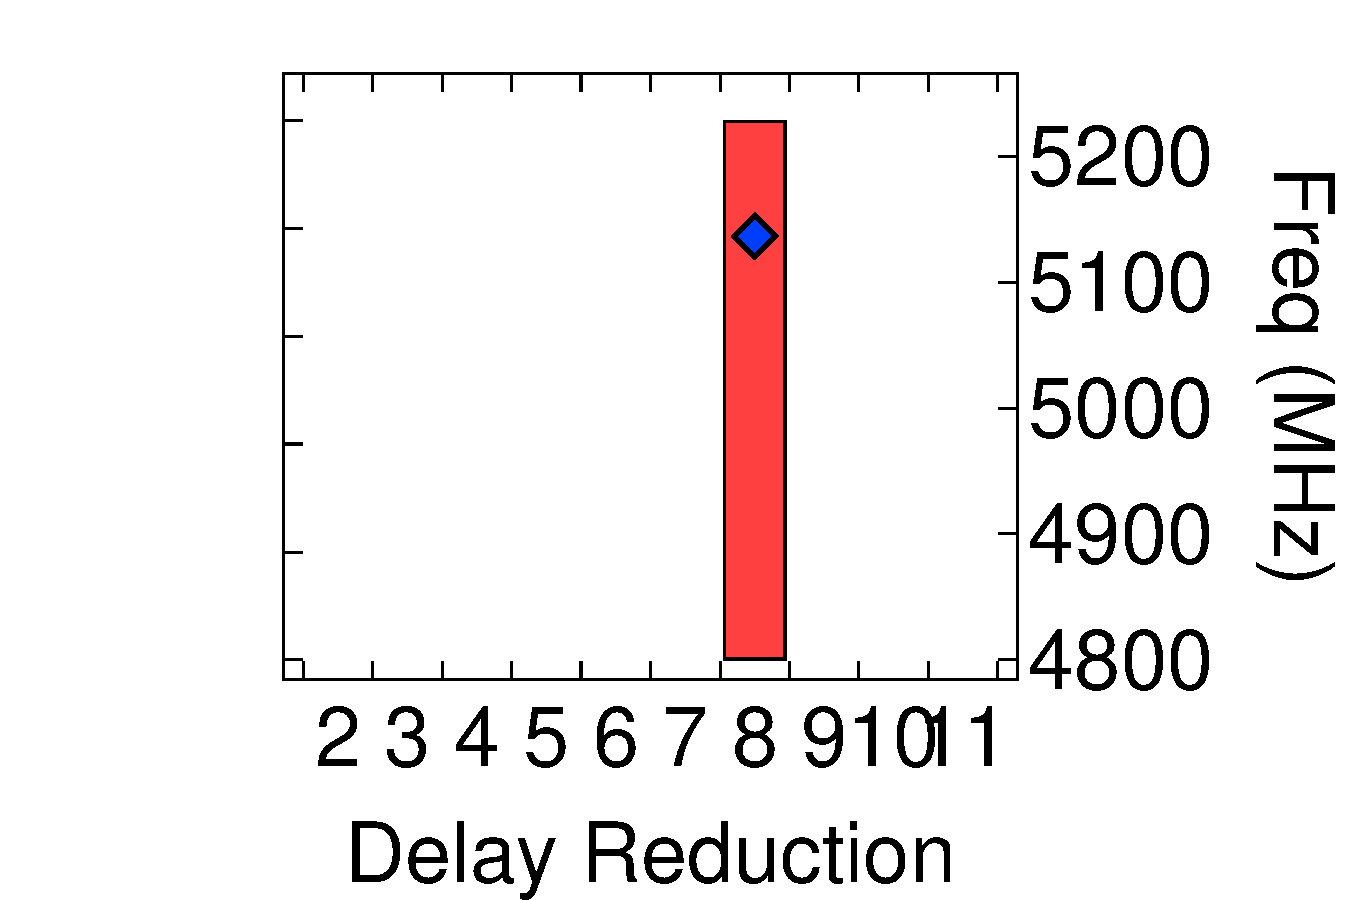
\includegraphics[trim=135 0 0 0,clip,width=.185\linewidth]{graphs/process/idle-limit-dist/idle-limit-dist-p1c3.pdf}
%        \label{fig:idle_dist_p1c3} 
%      }
%      \vspace{-0.1in}
%      \subfloat[p1 Core 4.] {
%        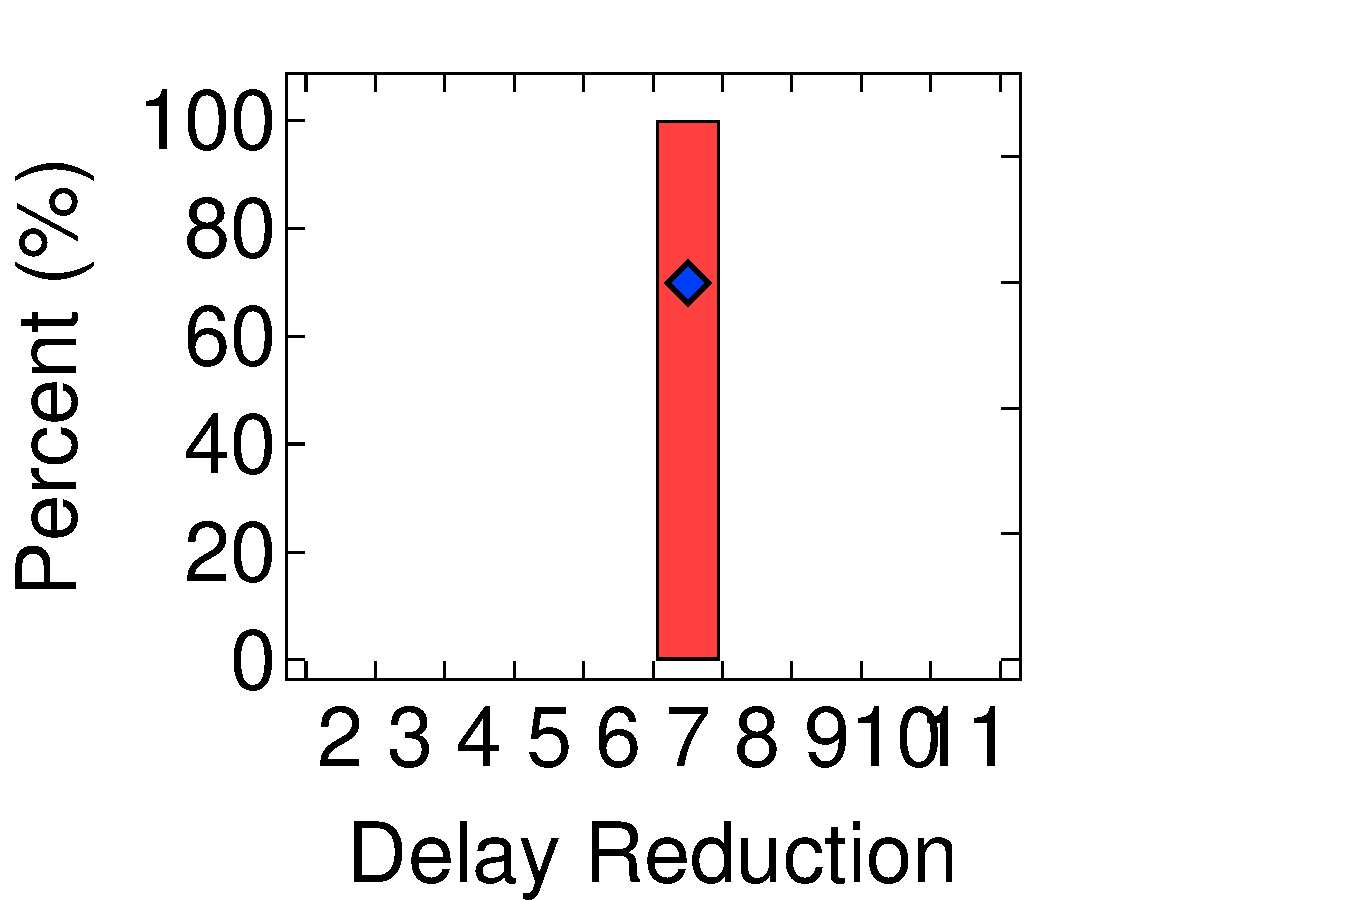
\includegraphics[trim=0 0 140 0,clip,width=.183\linewidth]{graphs/process/idle-limit-dist/idle-limit-dist-p1c4.pdf}
%        \label{fig:idle_dist_p1c4} 
%      }
%      %\hfill
%      \subfloat[p1 Core 5.] {
%        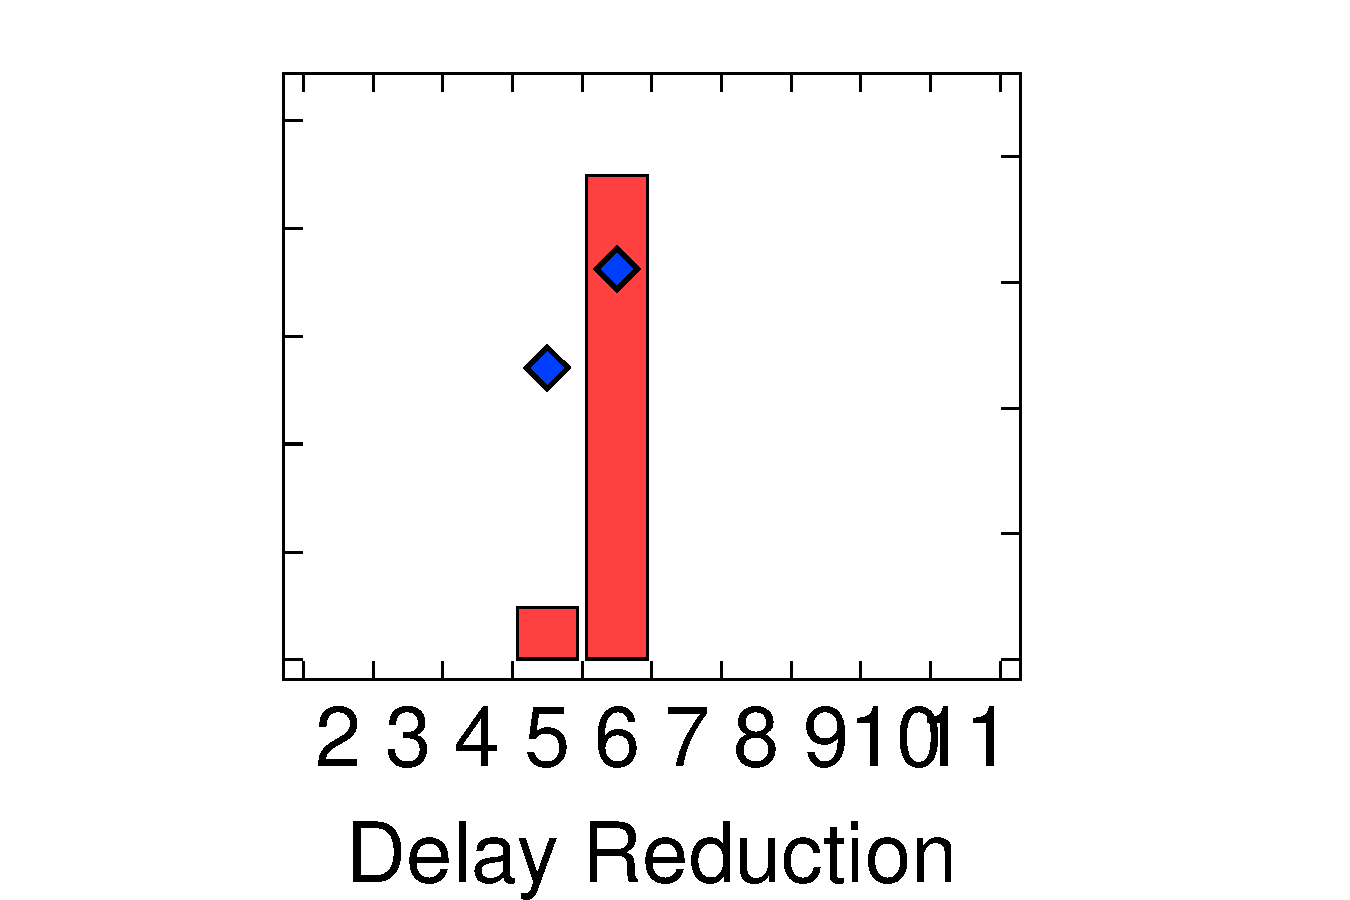
\includegraphics[trim=135 0 140 0,clip,width=.134\linewidth]{graphs/process/idle-limit-dist/idle-limit-dist-p1c5.pdf}
%        \label{fig:idle_dist_p1c5} 
%      }
%      %\hfill
%      \subfloat[p1 Core 6.] {
%        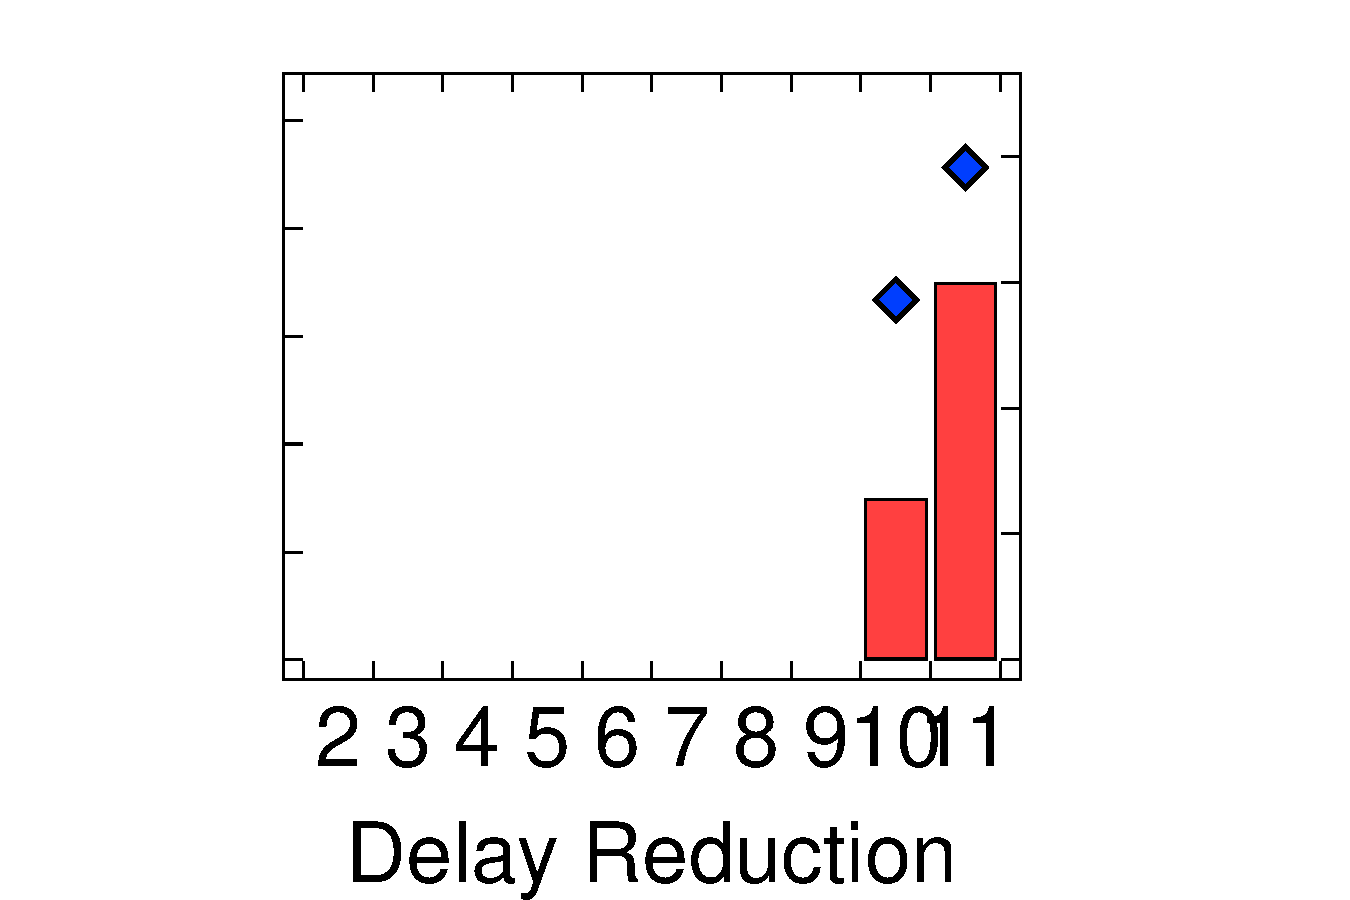
\includegraphics[trim=135 0 140 0,clip,width=.134\linewidth]{graphs/process/idle-limit-dist/idle-limit-dist-p1c6.pdf}
%        \label{fig:idle_dist_p1c6} 
%      }
%      %\hfill
%      \subfloat[p1 Core 7.] {
%        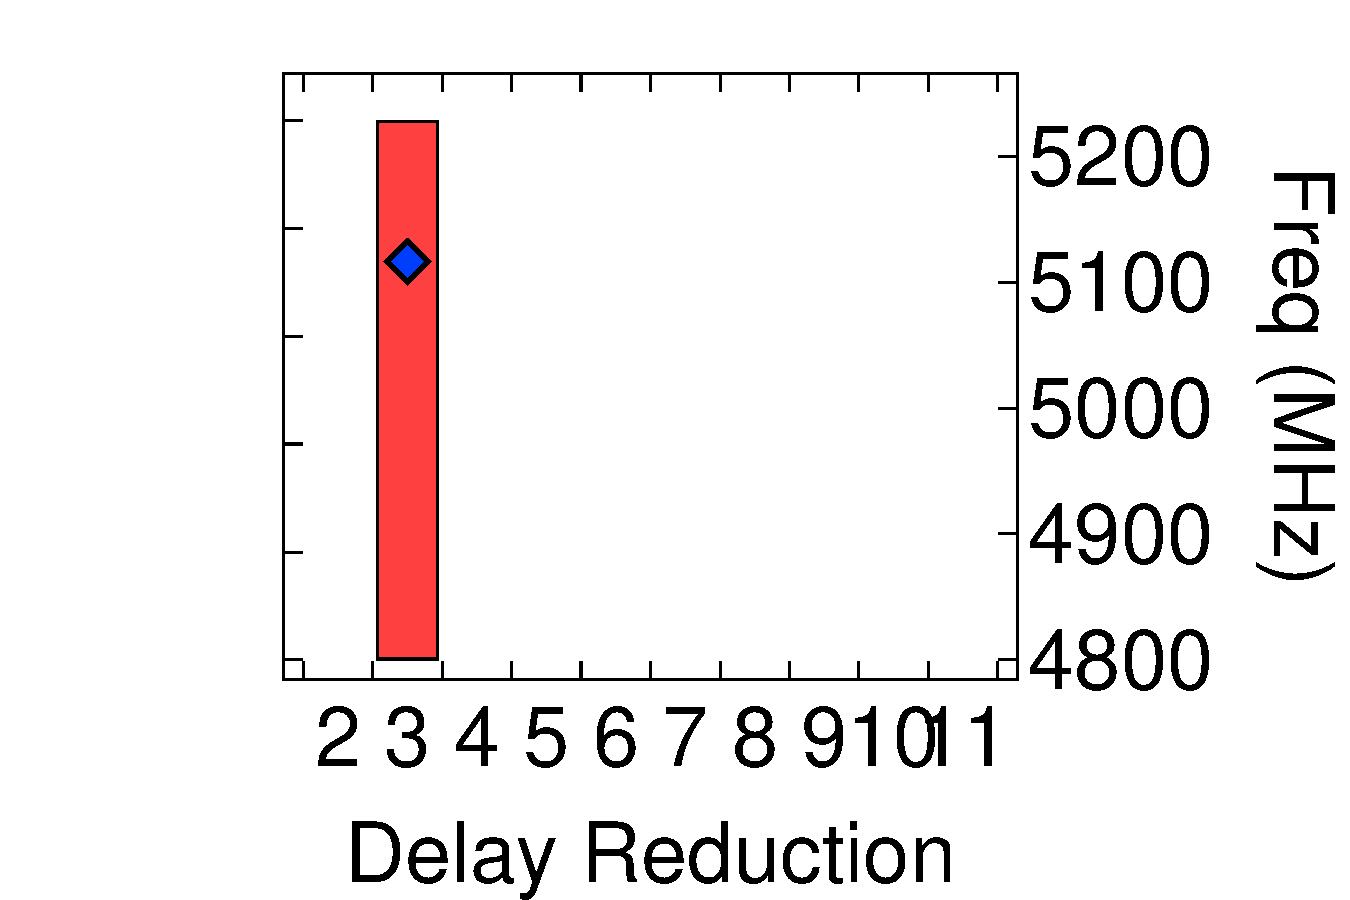
\includegraphics[trim=135 0 0 0,clip,width=.185\linewidth]{graphs/process/idle-limit-dist/idle-limit-dist-p1c7.pdf}
%        \label{fig:idle_dist_p1c7} 
%      }
%    \caption{The limit configuration of each POWER7+ core (i.e., the most aggressive reduction of CPM's inserted delay from its default setting, beyond which ATM operation can cause system failure under idle condition) distributes over a narrow range (red bar, left y axis). The operating frequency at each core's limit delay config is over 4800~MHz, more than 15\% higher than static margin's 4200~MHz level (blue mark, right y axis).}
   
%    \label{fig:idle-limit-dist} 
% \end{figure*}



\textbf{Realistic Workloads} %\paragraph{Single-threaded Benchmark}
For the final step, we profile the system with complex applications from SPEC CPU 2017 and PARSEC. These benchmarks cover a wide spectrum of program space in the real world and have diverse architecture behavior~\cite{song2018spec,bienia2008parsecsplash}; hence they can touch more corner-case timing paths or create more active $di/dt$ effects than uBench, all of which threatens the safe execution of aggressively reconfigured active timing margin. {The single-threaded workloads help identify application, chip-wide, and individual core level heterogeneity.}

In each of the above setups, failure may occur as a result of timing violation, manifested as an abnormal application termination (e.g., segmentation fault), silent data corruption (SDC), or a system crash. For SDC related error, we rely on SPEC and uBench's inherent result checking tool for guaranteeing execution correctness. All these failures may occur because either the CPM's delay has become so short that it does not capture real circuit delays or system noise events, such as the $di/dt$ effect, overwhelms the control loop's ability to respond in time. Because the effects that cause active timing margin failure might be not fully deterministic, we repeat the profiling in each setup multiple times to produce a distribution of active timing margin operating limits. We expect the distributions to be tight because timing violations will not be entirely random. These distributions provide a holistic view of active timing margin's margin reclamation capability, so we study them from here on.

Our methodology progresses through increasing workload complexity. Thus we often need to roll back the CPM delay setting that was successful in a previous less complex setup to a less aggressive point, reflecting a workload setup's unique impact on active timing margin's operation. Although the worst-case scenario might determine practical active timing margin reconfiguration in the real world, the middle point analysis shed useful insights on what affects the core-level customization of active timing margin's margin reclamation.

There is no guarantee that a particular circuit path or system noise event will deterministically lead to a timing violation, so we repeat the profiling in each of the above setups multiple times to produce a distribution of active timing margin operating limits. On the other hand, the effects that lead to a timing violation are not entirely random. Reconfiguring CPM inserted delay beyond a limit often leads to certain critical paths having much higher probabilities of experiencing timing errors; thus, the resulting distributions of successful CPM delays tend to be very tight. These distributions provide a holistic view of active timing margin's margin reclamation capability, so we study distributions here onward.

A timing violation manifests as an abnormal application termination (e.g., segmentation fault) or a system crash. It happens because either the CPM's delay has become so short that it does not capture real circuit delays, or system noise events, such as the $di/dt$ effect that overwhelms the DPLL.
%A timing violation manifests as either an abnormal application exit (e.g., early termination) or a system crash. These failures occur either because (1)~the removal of the CPM protection delay gives rise to a circuit path somewhere with a longer delay than that captured by the CPM; or (2)~system noise events, such as turbulence on the $V_{dd}$ power supply plane, undermine DPLL's ability to quickly slew frequency. 

Our profiling methodology progresses through increasingly complex workloads. Thus we often need to roll back the CPM delay setting to a less aggressive point, reflecting a workload's unique impact on active timing margin's operation.
%Each step of our profiling methodology builds upon the previous, less complex setup and so may result in failure where the previous step was successful. Thus we often need to roll back active timing margin operation to a less aggressive reclamation point by reconfiguring CPM inserted delays. The rollback delta reflects the workload's unique impact on active timing margin's aggressive operation.

\section{Idle System Characterization}
\label{sec:process:idle}

Understanding active timing margin's margin reclamation limits in an idle system sets a starting point for further, more complex analysis. With no application code running, the system exerts minimal stress on active timing margin's reconfigured control loop, enabling us to use active timing margin to expose the silicon's inherent maximum speed.

%We leverage the CPM delay reduction results in \Fig{fig:delay-freq} and incrementally reconfigure active timing margin to be more aggressive until the system fails. In this setting, failure occurs either because CPM reconfiguration removes the system's built-in protection delay and could give rise to a circuit path somewhere for which the CPM cannot adequately represent its timing delay or because system noise events such as turbulence on $V_{dd}$'s power supply plane makes the DPLL fail to slew frequency in time. Nevertheless, under many CPM reconfigurations, the more aggressive active timing margin still yields flawless execution.

Running only the operating system, we build a distribution of the most aggressive yet safe CPM configuration points for each core, depicted in \Fig{fig:idle-limit-dist} by the amount of CPM delay reduction from the chip's default setting, along with the resulting frequencies. As expected, the distributions are tight, covering no more than two configurations. Each core's \textit{idle limit} is the lowest (most conservative) CPM delay reduction plotted, e.g. 9 in \Fig{fig:idle_dist_p0c0}. These are summarized in \Tab{tab:limit-delay}. 

\begin{table*}[t]
\centering

% \begin{tabular}{l|c*{15}{c}}
% core               & P0C0 & P0C1 & P0C2 & P0C3 & P0C4  & P0C5 & P0C6 & P0C7 & P1C0 & P1C1 & P1C2 & P1C3 & P1C4  & P1C5 & P1C6 & P1C7\\
% \hline
% idle limit  & 9 & 8 & 4 & 11 & 10 & 7 & 8 & 2 & 4 & 8 & 5 & 8 & 7 & 5 & 10 & 3\\
% uBench limit & 9 & 8 & 4 & {\color{red} 10} & {\color{red}  9} & 7 & 8 & 2 & 4 & 8 & 5 & {\color{red} 5} & {\color{red} 6} & {\color{red} 4} & 10 & {\color{red} 2}\\
% SPEC normal & 8 & 7 & {\color{blue} 4} & 9 & 8 & 6 & 7 & {\color{blue} 2} & 3 & 7 & {\color{blue} 5} & 4 & 5 & 3 & 8 & {\color{blue} 2}\\
% SPEC worst & 7 & 6 & 3 & 6 & 6 & 5 & 5 & {\color{ForestGreen} 2} & {\color{ForestGreen} 3} & 3 & {\color{ForestGreen} 5} & 3 & 3 & 2 & 6 & {\color{ForestGreen} 2}\\
% \end{tabular}
%\vspace{0.2cm}
%\caption{Extreme CPM delay reduction step that makes system stable. Under ubench stress, the highlighted cores' (e.g., P0C3) limit delays are rolled back from their idle config because uBench stresses paths more completely and hits paths untested when idle. The uBench-tested delay config makes the aggressive ATM system more reliable. }

\resizebox{\textwidth}{!}{
\begin{tabular}{l|c*{15}{c}}
               & P0C0 & P0C1 & P0C2 & P0C3 & P0C4  & P0C5 & P0C6 & P0C7 & P1C0 & P1C1 & P1C2 & P1C3 & P1C4  & P1C5 & P1C6 & P1C7\\
\hline
idle limit  & 9 & 8 & 4 & 11 & 10 & 7 & 8 & 2 & 4 & 8 & 5 & 8 & 7 & 5 & 10 & 3\\
uBench limit & 9 & 8 & 4 & 10 & 9 & 7 & 8 & 2 & 4 & 8 & 5 & 5 & 6 & 4 & 10 & 2\\
thread normal & 8 & 7 & 4 & 9 & 8 & 6 & 7 & 2 & 3 & 7 & 5 & 4 & 5 & 3 & 8 & 2\\
thread worst & 6 & 6 & 3 & 6 & 6 & 5 & 5 & 2 & 3 & 3 & 5 & 3 & 3 & 2 & 6 & 2\\
\end{tabular}
}
\vspace{0.2cm}
\caption{ATM customization limits under system idle, uBench, and real-world application. Data is collected on two eight-core (C) POWER7+ processors (P). ATM limits are reflected as the number of stepped reduced from CPM's default inserted delay configuration.}

%From system idle to uBench test, six cores' CPM delay need to be rolled back to guarantee successful run. Most SPEC and PARSEC workloads need one extra roll-back step to pass. Problematic workloads, such as \bench{x264} and \bench{ferret} needs more roll back at the cost of smaller overclocking benefits.

\label{tab:limit-delay} 
\vspace{-0.3cm}
\end{table*}


The different core-to-core idle limits reveal lucrative performance potential for aggressive active timing margin customization (\Sec{sec:process:idle:potential}), and the significant core-to-core performance variation (\Sec{sec:process:idle:heterogeneity}) which is partly caused by the non-linearity in CPM configuration (\Sec{sec:process:idle:cpm_variation}).

\subsection{Significant Performance Potential}
\label{sec:process:idle:potential}

For most cores, the inserted delay can be aggressively reduced, making active timing margin's control loop see more timing margin for reclamation. As \Fig{fig:idle-limit-dist} shows, more than half the cores (e.g., P0C0 and P0C1) can tolerate reductions of at least seven steps of CPM inserted delay, elevating frequencies to over 5000~MHz: a 7\% improvement over default active timing margin's 4600~MHz and a 20\% improvement over static margin's 4200~MHz baseline, showing customized active timing margin can substantially improve performance.

\subsection{Exposed Inter-core Frequency Variation}
\label{sec:process:idle:heterogeneity}

Programming the CPM to change active timing margin operation yields different frequency levels for each core, despite the performance improvement. For instance, at the idle limit P1C2 runs at about 4850~MHz but P0C3 achieves about 5200~MHz. Even within a chip, there is a wide range (e.g., P0C2 and P0C3). The core-to-core frequency variation is essential for application performance management, which we discuss later.

The core to core differences are understood to be a result of manufacturing process variations~\cite{dighe2010within,rangan2011achieving}, i.e., some core's circuits are faster due to imperfection in the lithography process. For instance, as \Fig{fig:idle-limit-dist} shows, P0C3 can safely reduce its CPM delay by 11 steps, while P0C7 can only mitigate its delay by two, reflecting the varying amount of timing margin available for reclamation, which is caused by the two cores' speed difference.

However, because on the POWER7+ each core's performance potential is unlocked via active timing margin control loop's automatic harness of available timing margin, the functioning of active timing margin control loop also plays a critical role in the inter-core performance variation.

\subsection{Nonlinearity of CPM Configuration}
\label{sec:process:idle:cpm_variation}

The CPM inserted delay's configurable inverter chain is designed to have linear timing delay graduation for timing margin measurement. However, the manufacturing process makes it have non-linear graduation when configured to measure timing margin. The non-linearity magnifies the inter-core performance heterogeneity.

The inserted delay's non-linear configuration manifests as significant idle limit variation between cores. Consider P0C4 and P1C7, which are both able to increase frequency from 4600~MHz to 5100~MHz but do so with very different CPM changes: P0C4 reduces the delay by ten steps, while P1C7 only needs two steps. Hence, although the two cores have similar excess timing margins, P0C4's CPM encodes smaller timing delays in each step than P1C7. 

Within each core, CPM's non-linearity makes the timing margin encoded by one CPM delay step vary. \Fig{fig:delay-freq} shows that P1C6's frequency increases by over 200~MHz when going from step zero to one, jumping from the baseline 4600~MHz to over 4800~MHz. But in going from step one to two, there is an almost negligible change in frequency. Similarly, the frequency is nearly unchanged when increasing the CPM delay reduction from step five to six for P1C3, but reducing the delay by one additional step (i.e., going from six to seven) increases the frequency by over 100~MHz.

As another example, in \Fig{fig:idle_dist_p1c2} reducing P1C2's CPM delay by six is too aggressive and can crash the system; rolling back its delay by one step ensures safety but at the cost of 300~MHz. P1C1 (\Fig{fig:idle_dist_p1c1}) similarly needs its CPM delay reduction rolled back by one step (from nine to eight) for safe operation but at the cost of only 100~MHz. Though P1C2 could operate safely at a higher frequency, the large CPM jump forces the 300~MHz drop and amplifies the differences between the two cores.

In summary, the non-linearity configuration of the CPM and active timing margin control loop demands that customization of multi-core Active Timing Margin operation be carried out carefully on the per-core basis because no single CPM configuration works uniformly for all cores.

\section{Micro-bench Characterization}
\label{sec:process:ubench}

\begin{figure*}[t]
      \subfloat[p0 core3, \bench{daxpy}] {
        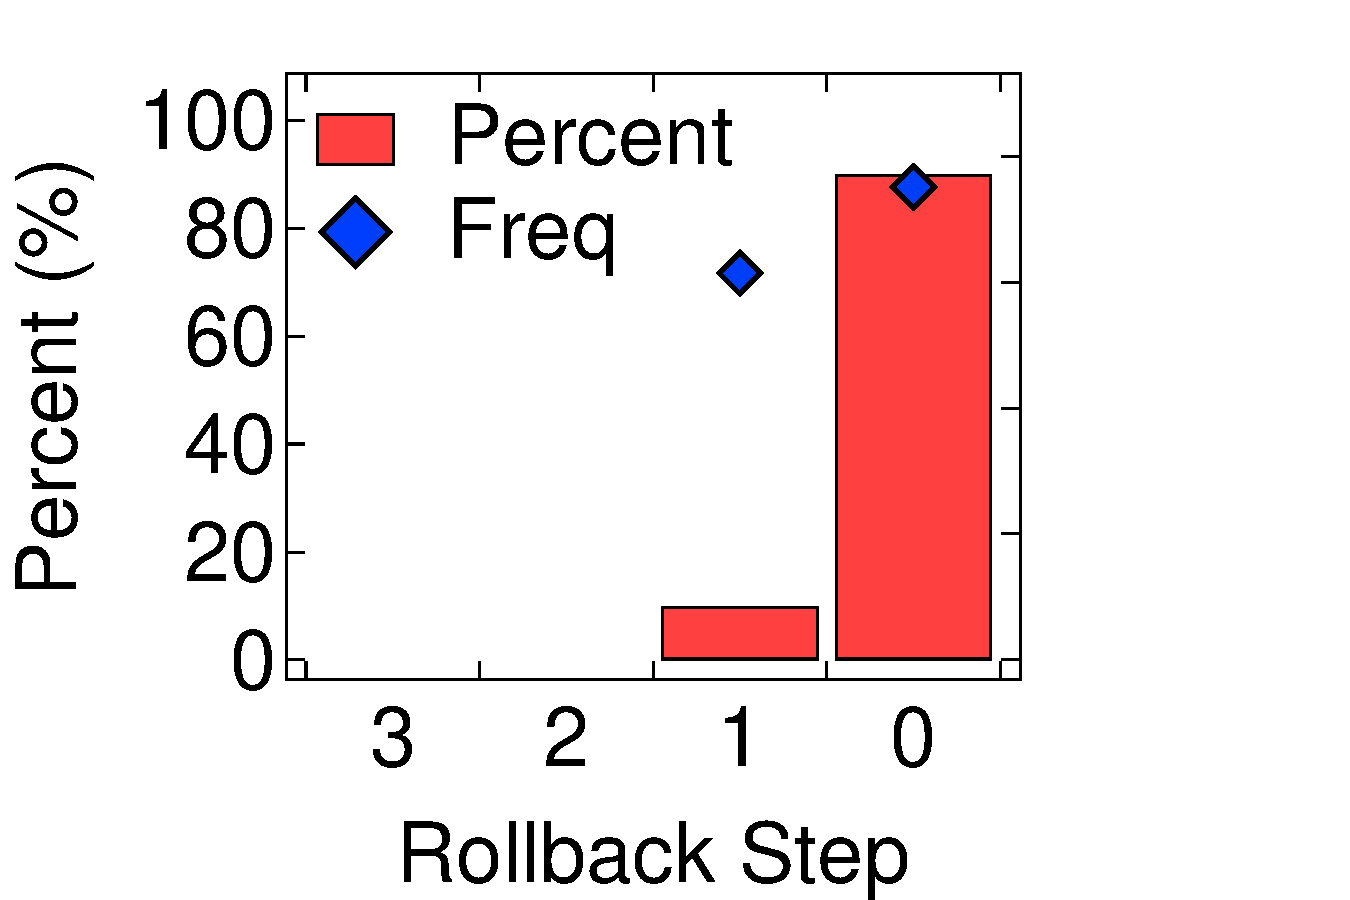
\includegraphics[trim=0 0 0 0,clip,width=.3\linewidth]{graphs/process/ubench-limit-dist/fp-limit-dist-p0c3.pdf}
      }
      \hfill
      \subfloat[p0 core4, \bench{daxpy}] {
        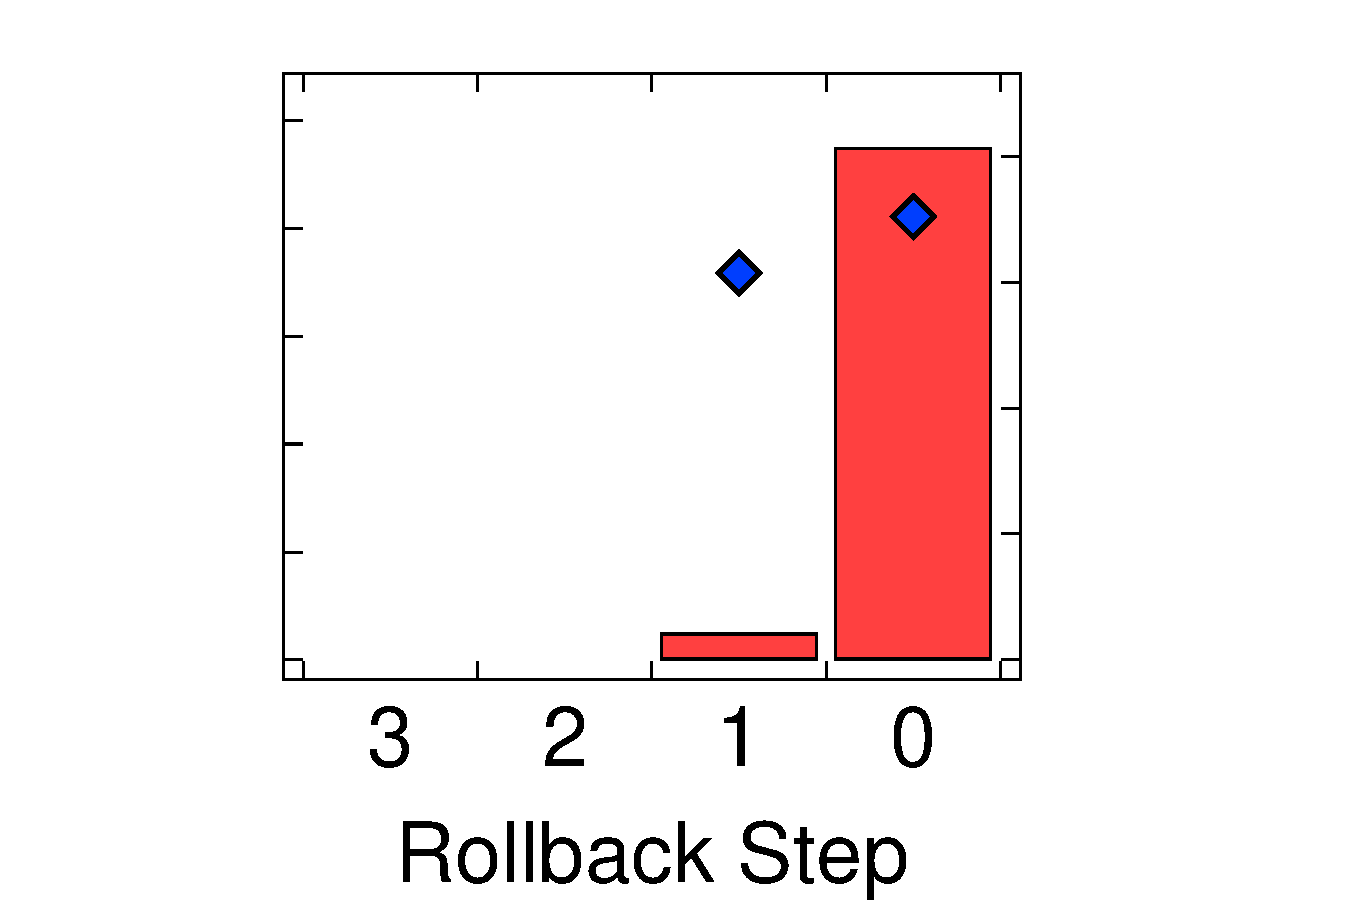
\includegraphics[trim=0 0 0 0,clip,width=.3\linewidth]{graphs/process/ubench-limit-dist/fp-limit-dist-p0c4.pdf}
      }
      \hfill
      \subfloat[p1 core3, \bench{stream}] {
        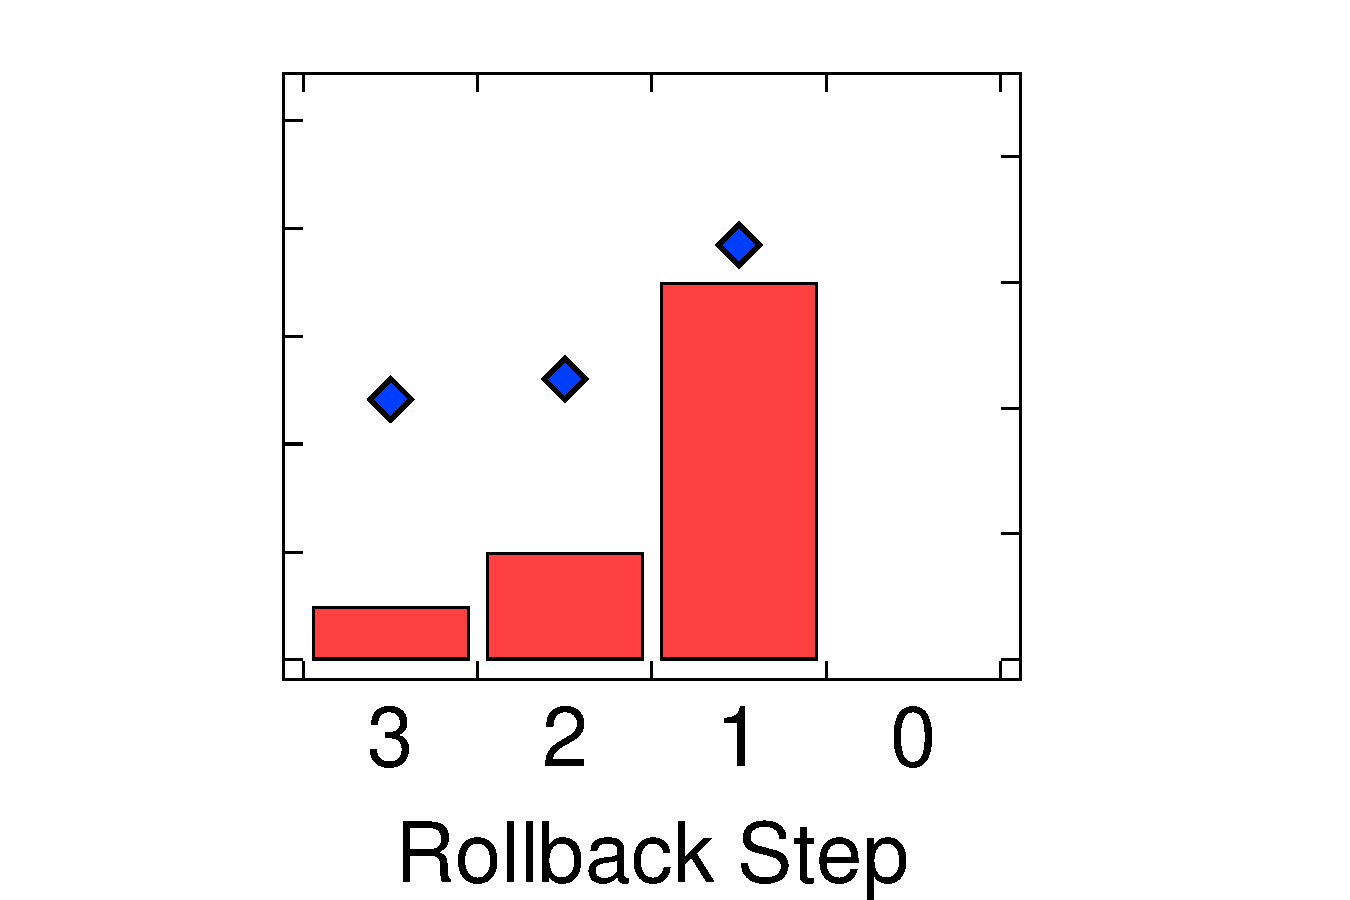
\includegraphics[trim=0 0 0 0,clip,width=.3\linewidth]{graphs/process/ubench-limit-dist/mem-limit-dist-p1c3.pdf}
      }

      \subfloat[p1 core4, \bench{stream}] {
        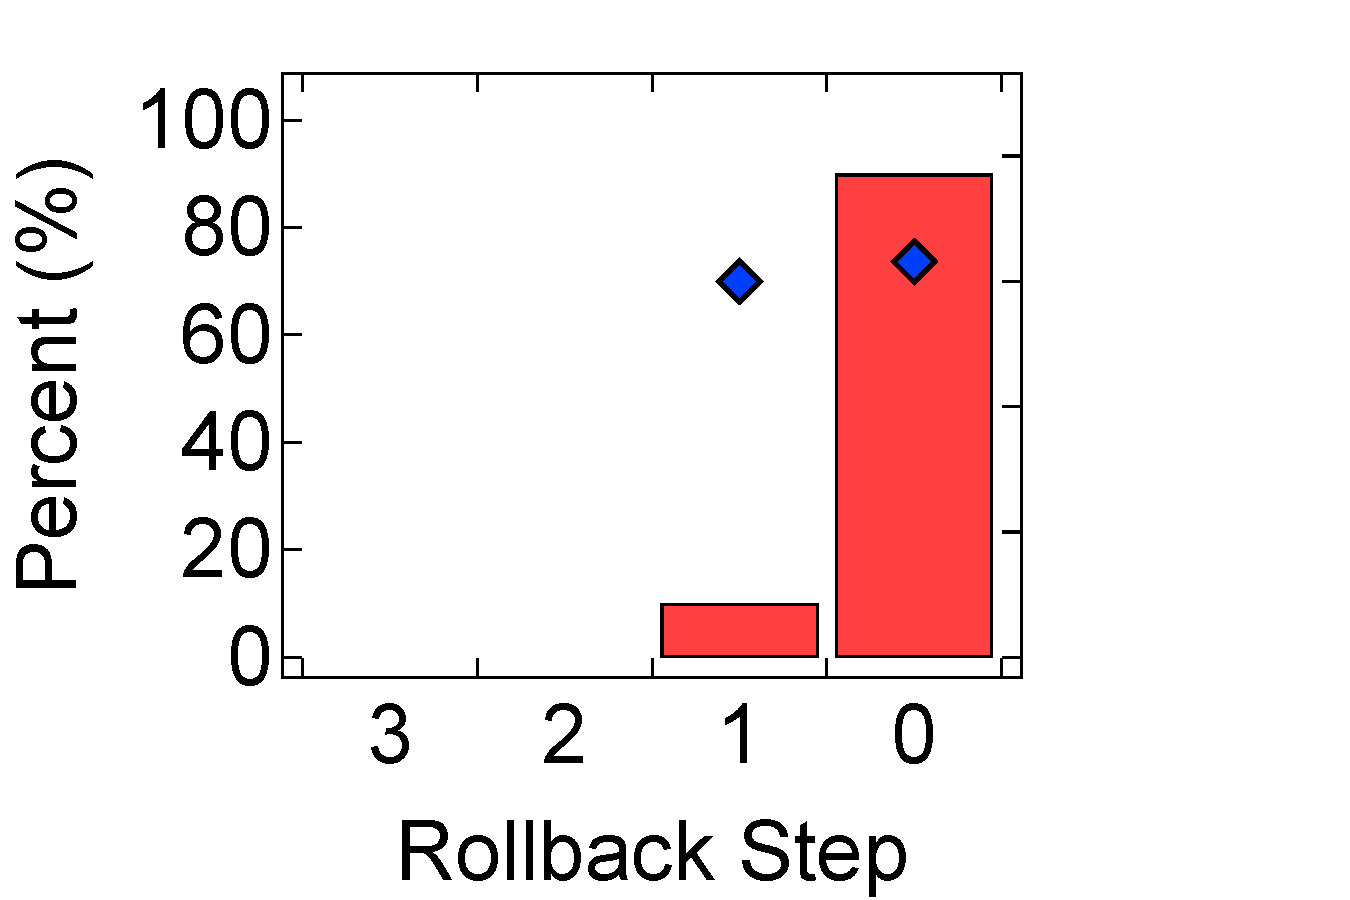
\includegraphics[trim=0 0 0 0,clip,width=.3\linewidth]{graphs/process/ubench-limit-dist/mem-limit-dist-p1c4.pdf}
      }
      \hfill
      \subfloat[p1 core5, \bench{coremark}] {
        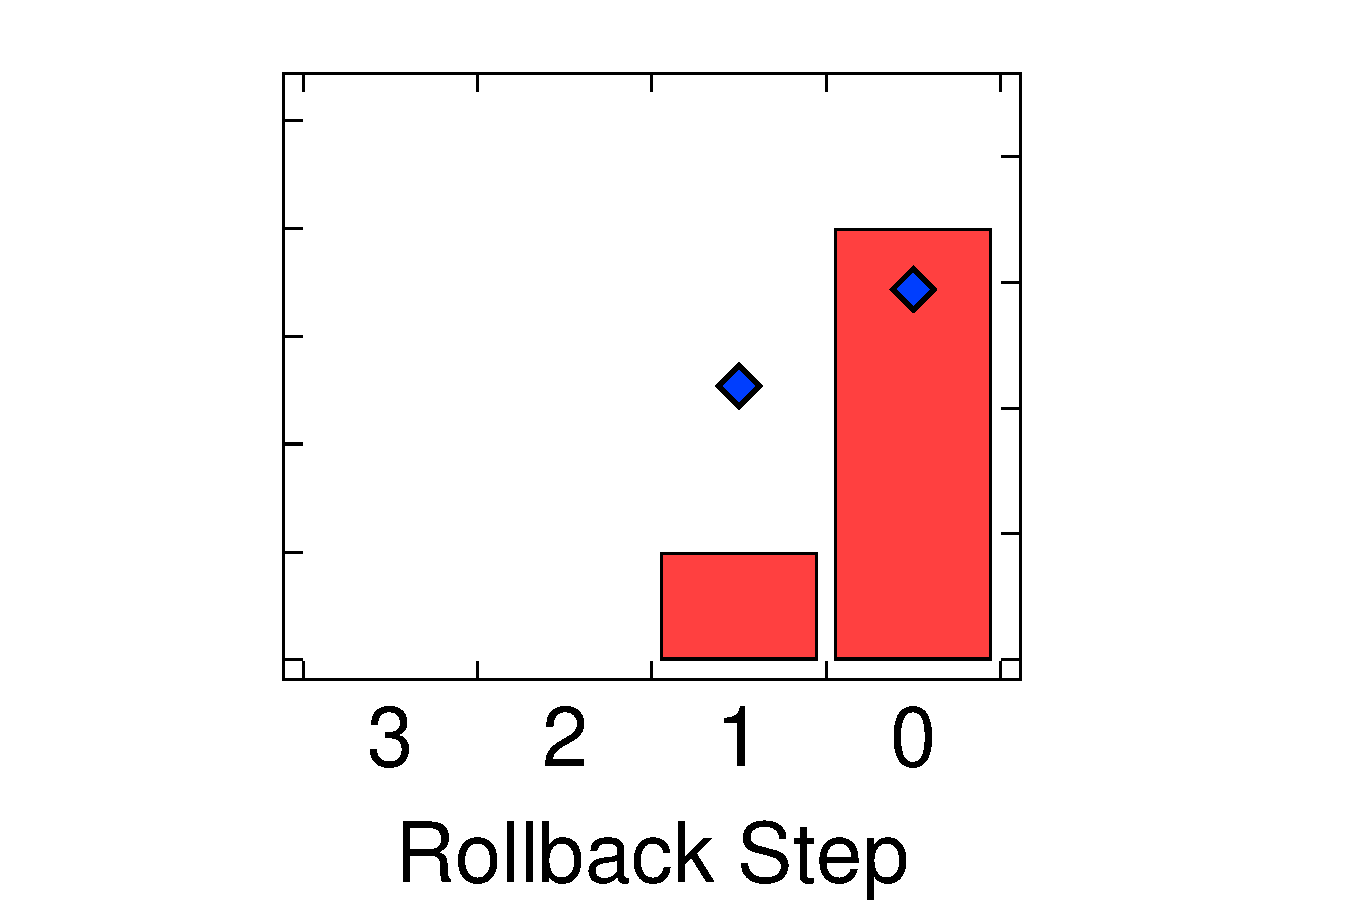
\includegraphics[trim=0 0 0 0,clip,width=.3\linewidth]{graphs/process/ubench-limit-dist/int-limit-dist-p1c5.pdf}
      }
      \hfill
      \subfloat[p1 core7, \bench{coremark}] {
        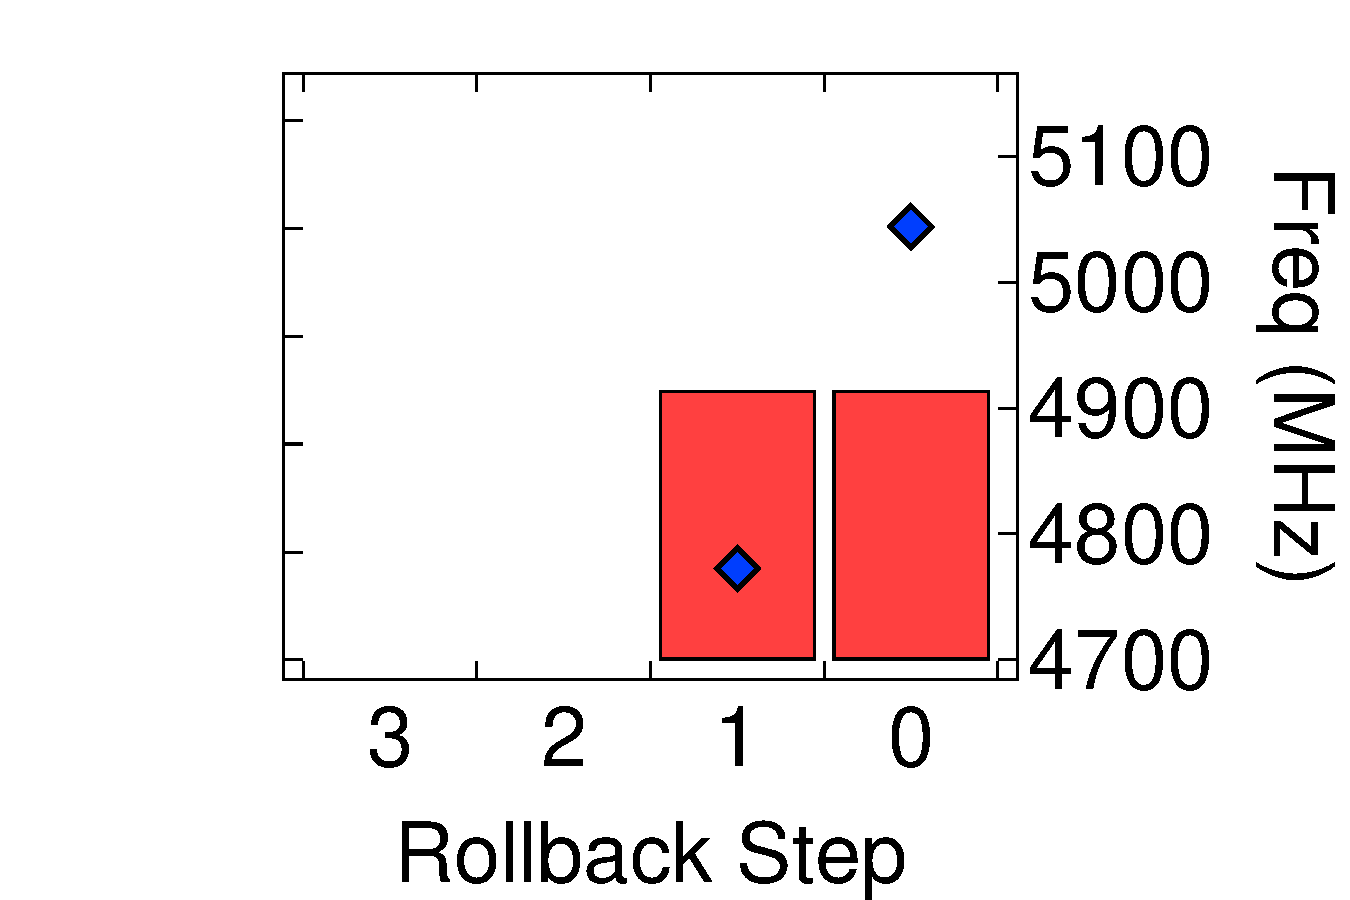
\includegraphics[trim=0 0 0 0,clip,width=.3\linewidth]{graphs/process/ubench-limit-dist/int-limit-dist-p1c7.pdf}
      }
    \caption{For 6 out of 16 cores, ATM configuration (i.e., CPM's inserted delay setting) needs to be rolled back from its idle limit in order for micro-benchmark (uBench) to run successfully. The 
    FP (\bench{daxpy}), MEM (\bench{stream}), and INT (\bench{coremark}) uBench have similar distribution of their pass config, indicating the core's mismatch between its reconfigured CPM timing measurement and its actual circuit speed. The other 10 cores not shown can run uBench safely at their idle limits.}
    \label{fig:ubench-limit-dist} 
\end{figure*}

%\begin{figure*}[t]
%      \subfloat[p0c3, \bench{daxpy}] {
%        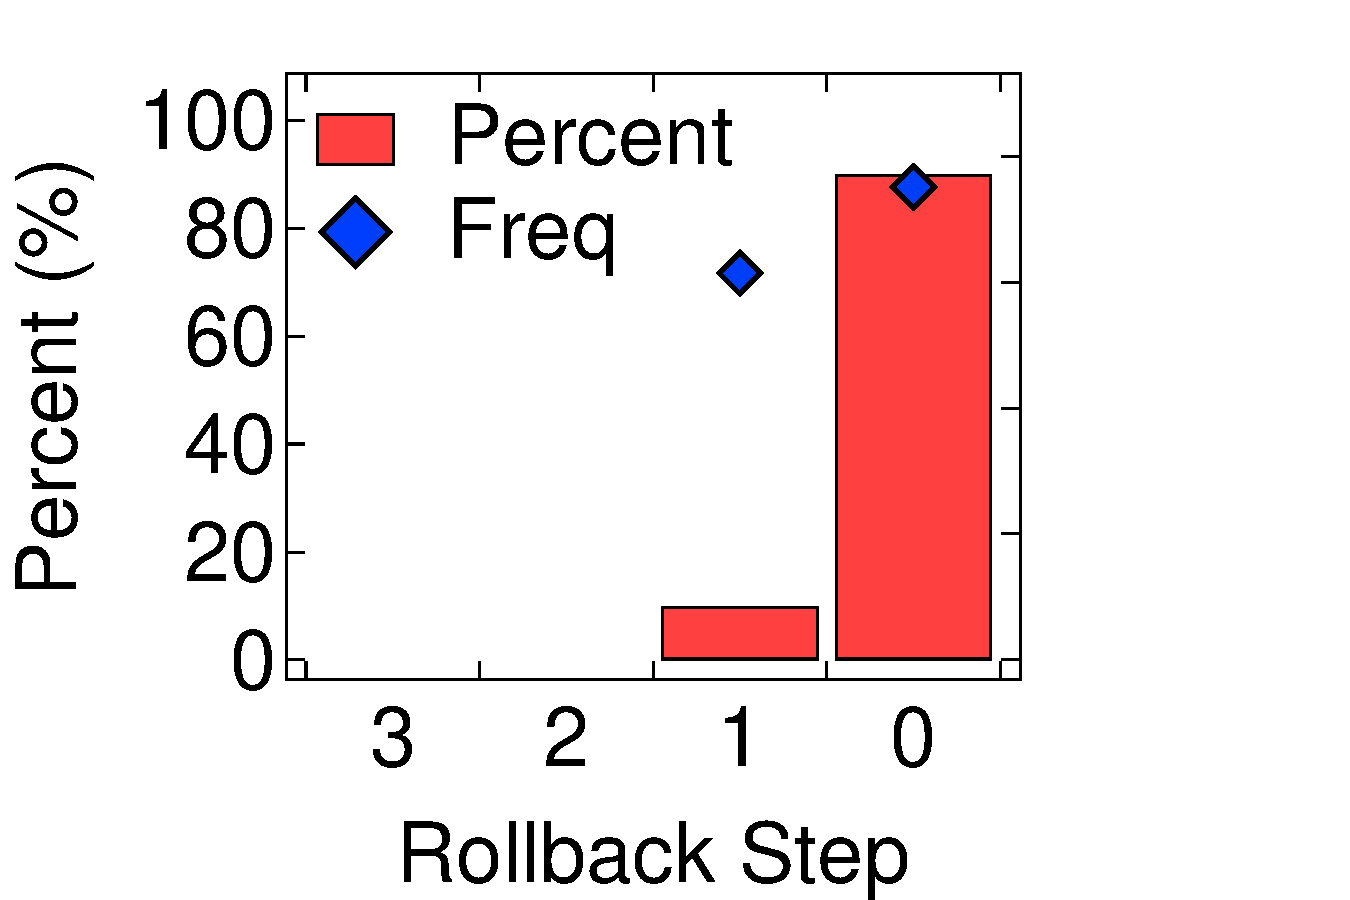
\includegraphics[trim=0 0 150 0,clip,width=.180\linewidth]{graphs/process/ubench-limit-dist/fp-limit-dist-p0c3.pdf}
%      }
%      \hfill
%      \subfloat[p0c4, \bench{daxpy}] {
%        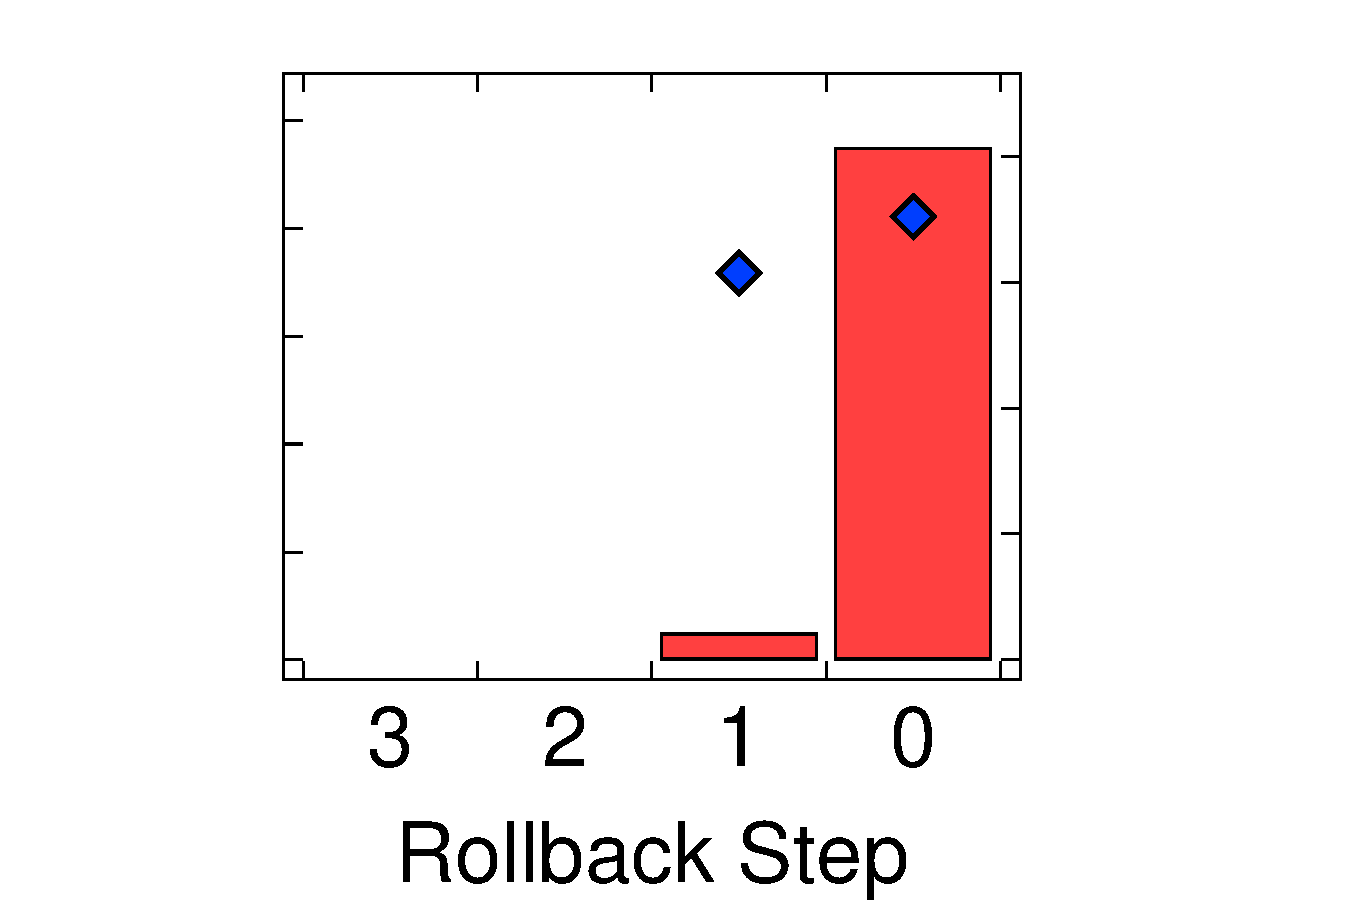
\includegraphics[trim=130 0 150 0,clip,width=.132\linewidth]{graphs/process/ubench-limit-dist/fp-limit-dist-p0c4.pdf}
%      }
%      \hfill
%      \subfloat[p1c3, \bench{stream}] {
%        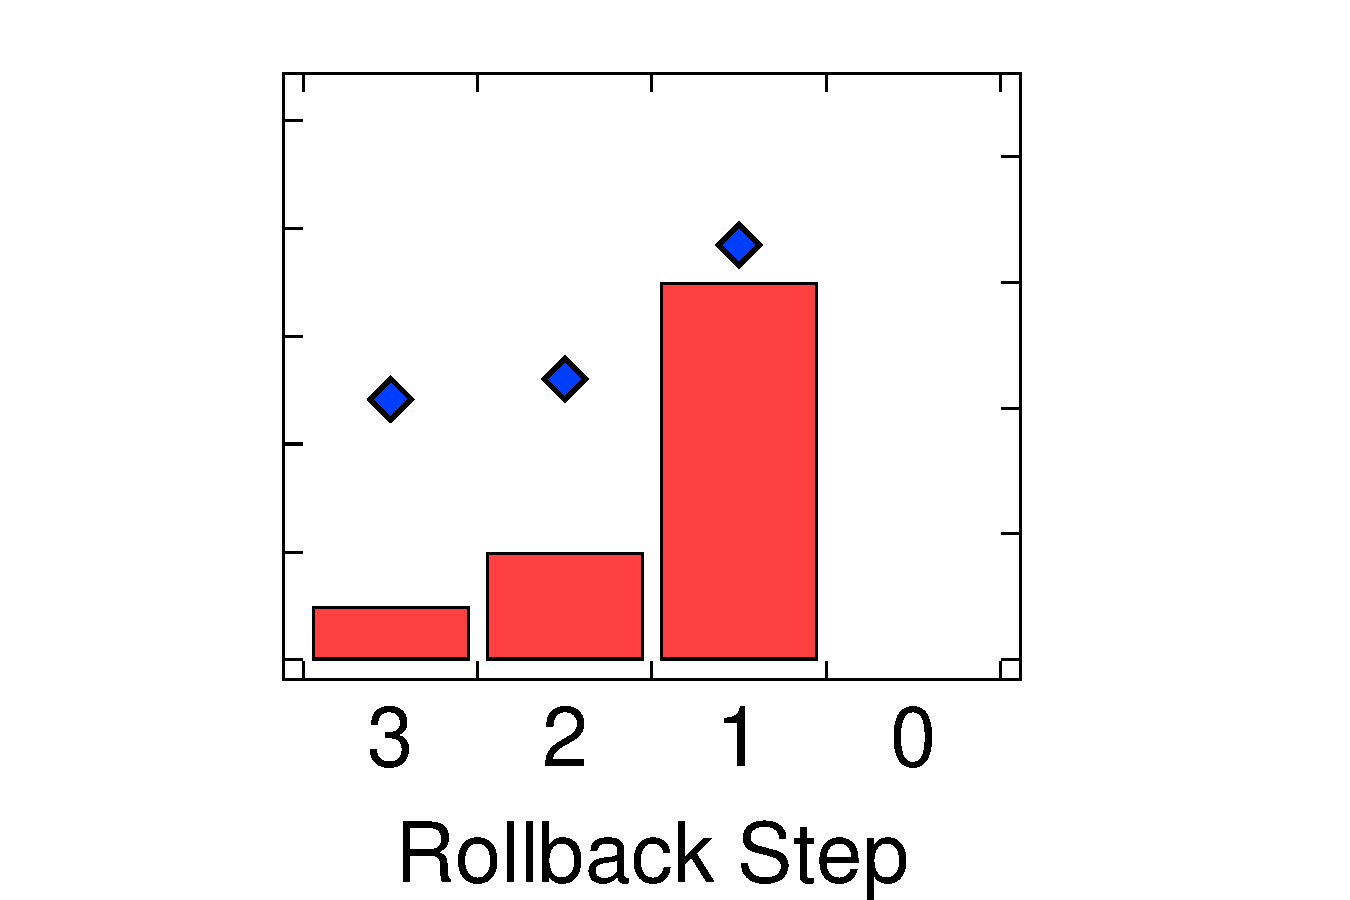
\includegraphics[trim=130 0 150 0,clip,width=.132\linewidth]{graphs/process/ubench-limit-dist/mem-limit-dist-p1c3.pdf}
%      }
%      \hfill
%      \subfloat[p1c4, \bench{stream}] {
%        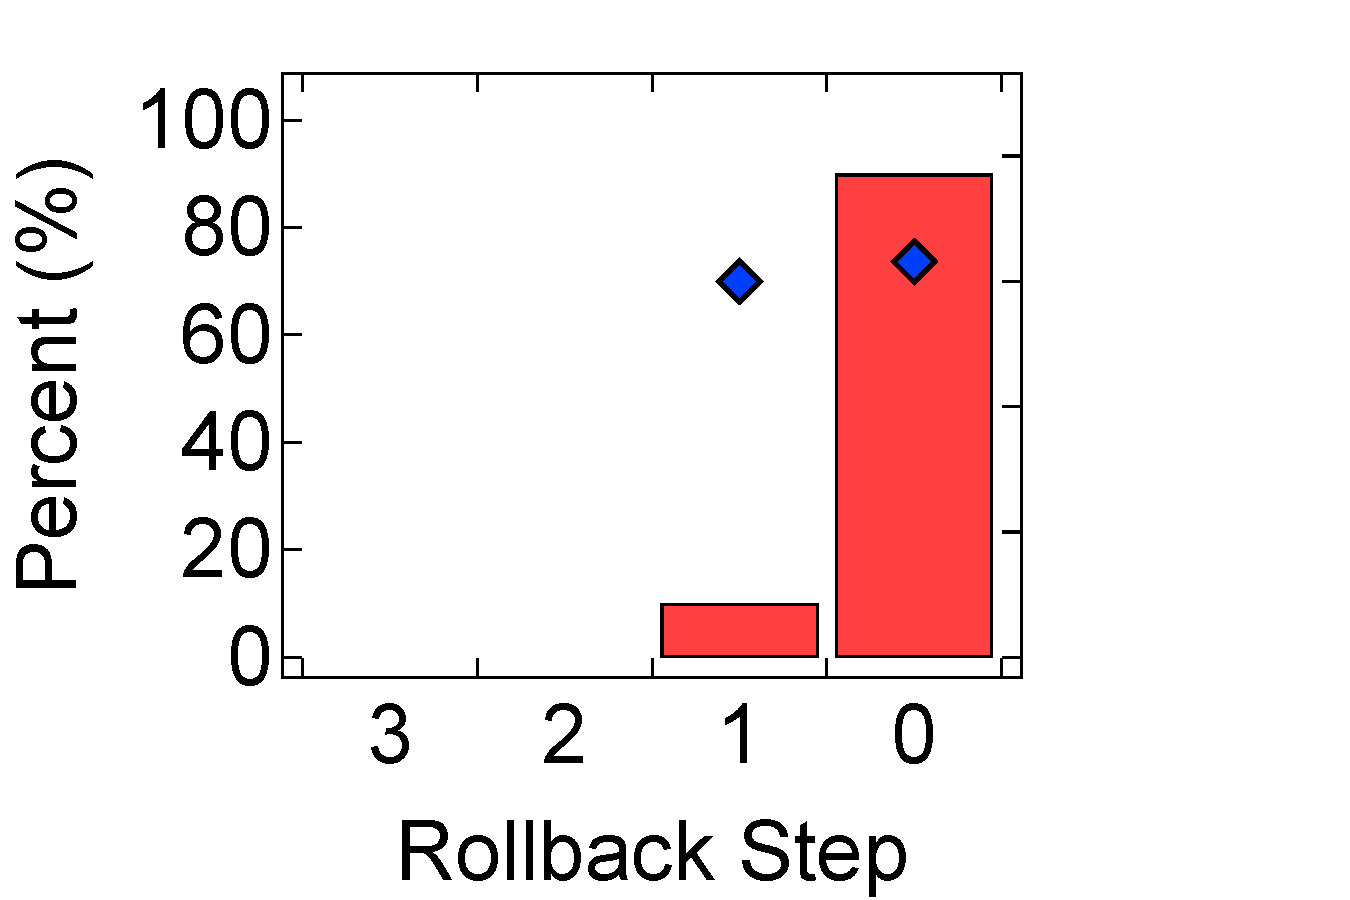
\includegraphics[trim=130 0 150 0,clip,width=.132\linewidth]{graphs/process/ubench-limit-dist/mem-limit-dist-p1c4.pdf}
%      }
%      \hfill
%      \subfloat[p1c5, \bench{coremark}] {
%        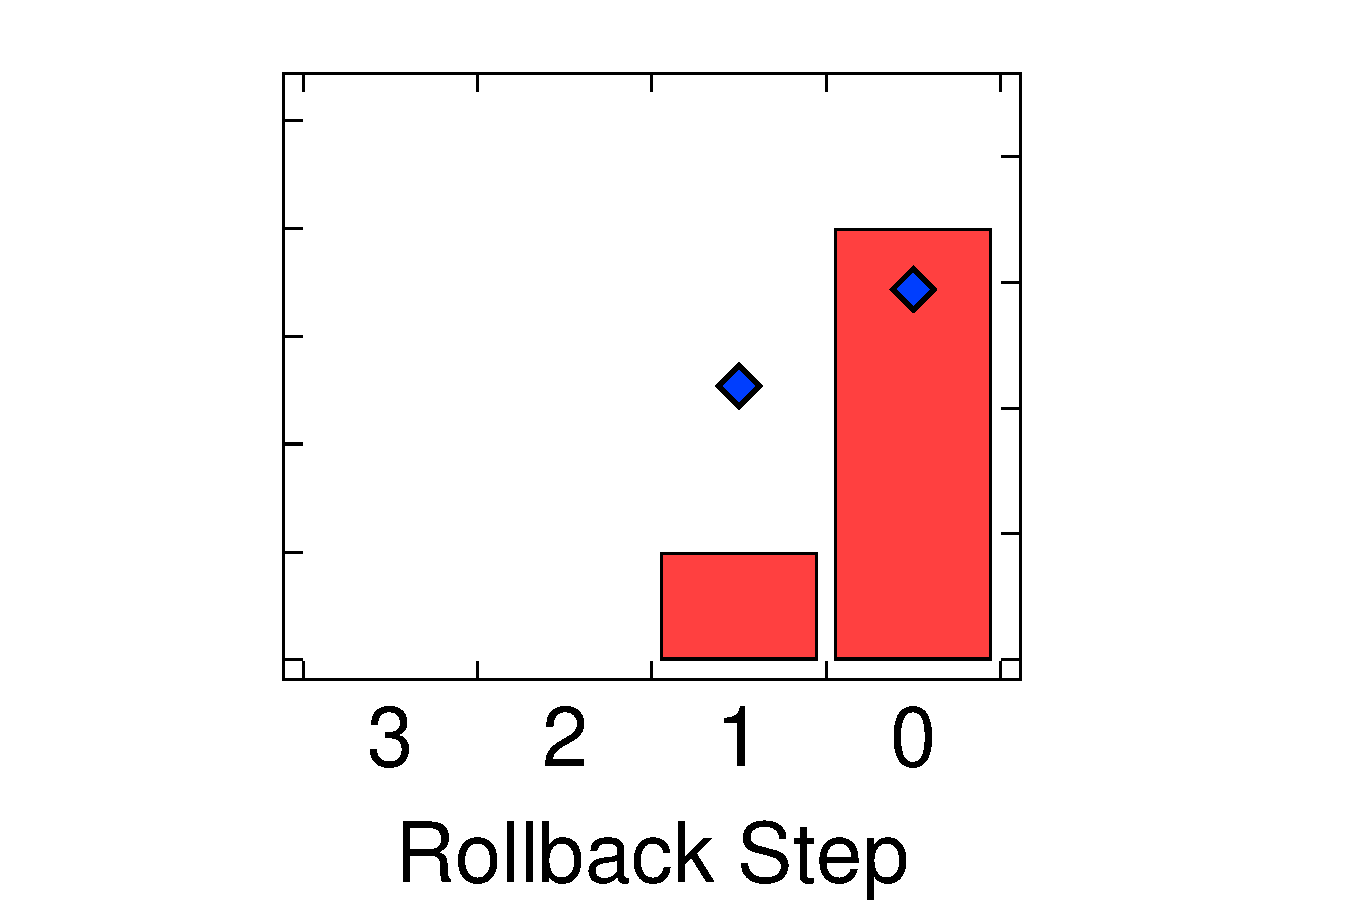
\includegraphics[trim=130 0 150 0,clip,width=.132\linewidth]{graphs/process/ubench-limit-dist/int-limit-dist-p1c5.pdf}
%      }
%      \hfill
%      \subfloat[p1c7, \bench{coremark}] {
%        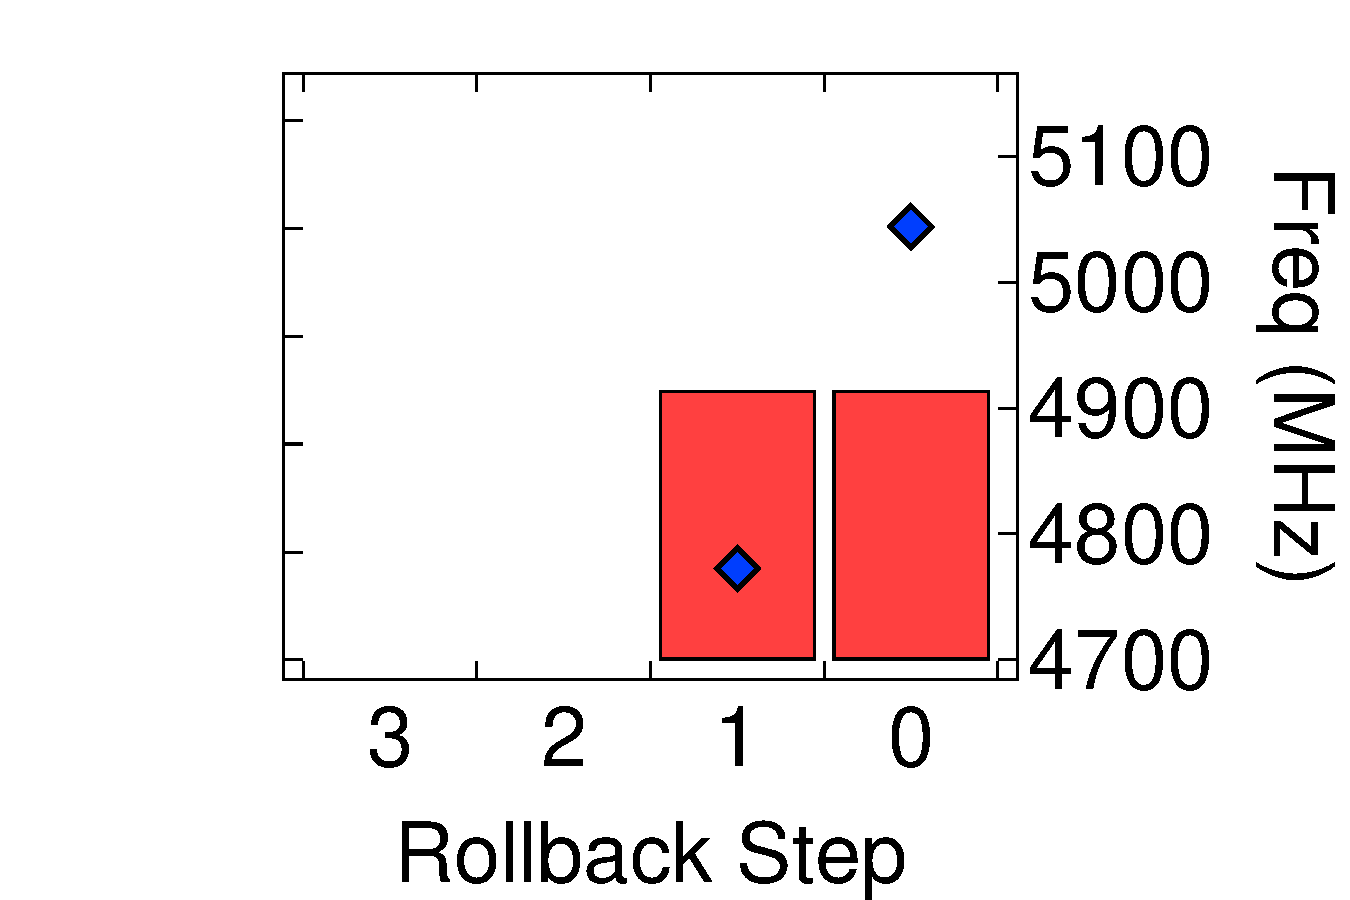
\includegraphics[trim=130 0 0 0,clip,width=.186\linewidth]{graphs/process/ubench-limit-dist/int-limit-dist-p1c7.pdf}
%      }
%    \caption{For 6 out of 16 cores, ATM configuration (i.e., CPM's inserted delay setting) needs to be rolled back from its idle limit in order for micro-benchmark (uBench) to run successfully. The 
%    FP (\bench{daxpy}), MEM (\bench{stream}), and INT (\bench{coremark}) uBench have similar distribution of their pass config, indicating the core's mismatch between its reconfigured CPM timing measurement and its actual circuit speed. The other 10 cores not shown can run uBench safely at their idle limits.}
%    \label{fig:ubench-limit-dist} 
%\end{figure*}

% \begin{figure*}[t]
%     \captionsetup[subfigure]{font=footnotesize}
%     \begin{subfigure}{.180\linewidth}
%         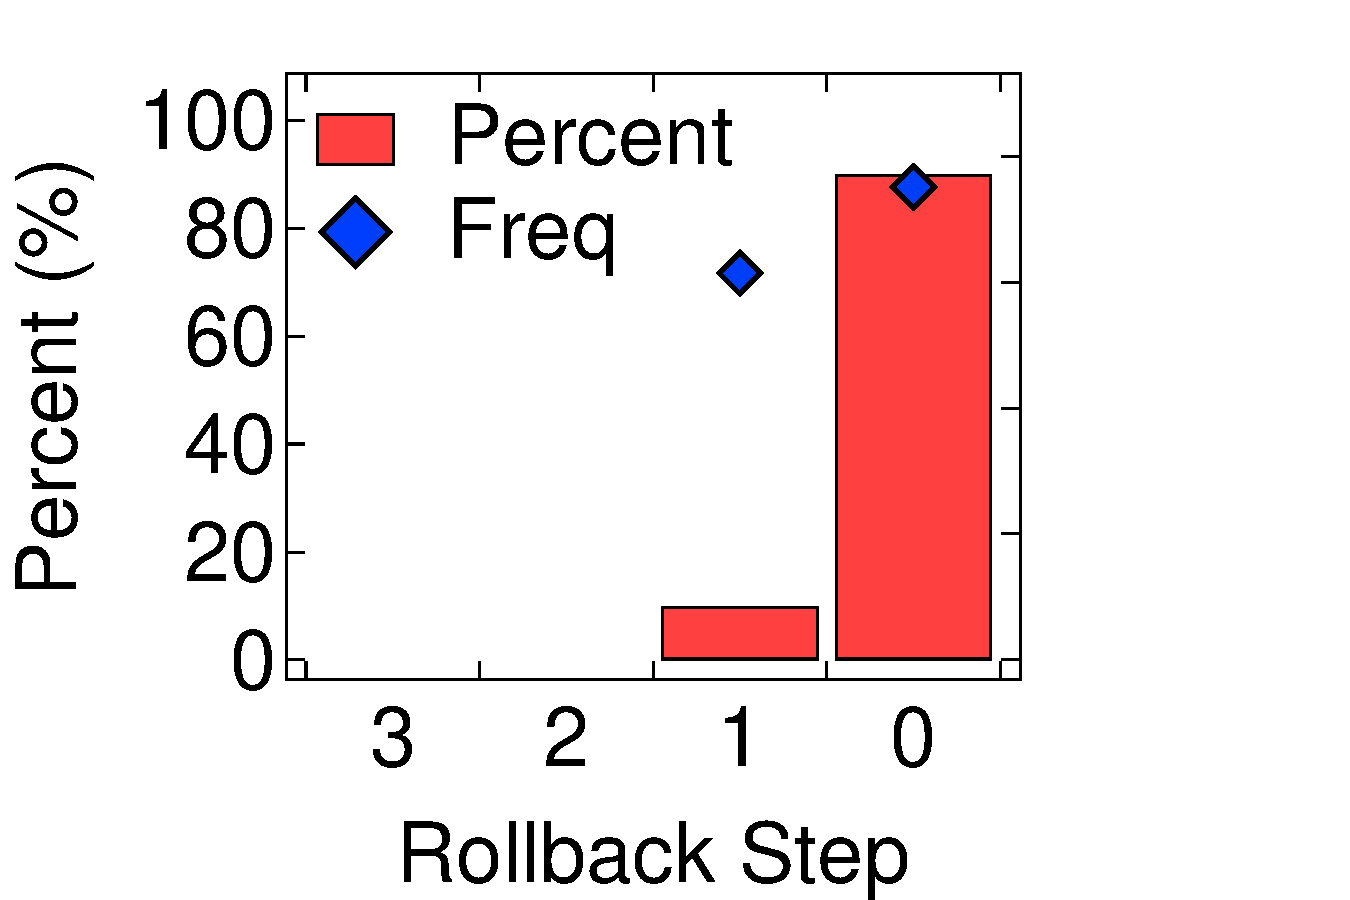
\includegraphics[trim=0 0 150 0,clip,width=\linewidth]{graphs/process/ubench-limit-dist/fp-limit-dist-p0c3.pdf}
%         \setlength{\abovecaptionskip}{-9pt}
%         \captionsetup{oneside,margin={23pt,0pt}}
%         \caption{P0C3, \\\bench{daxpy}}
%     \end{subfigure}
%     \hfill
%     \begin{subfigure}{.132\linewidth}
%         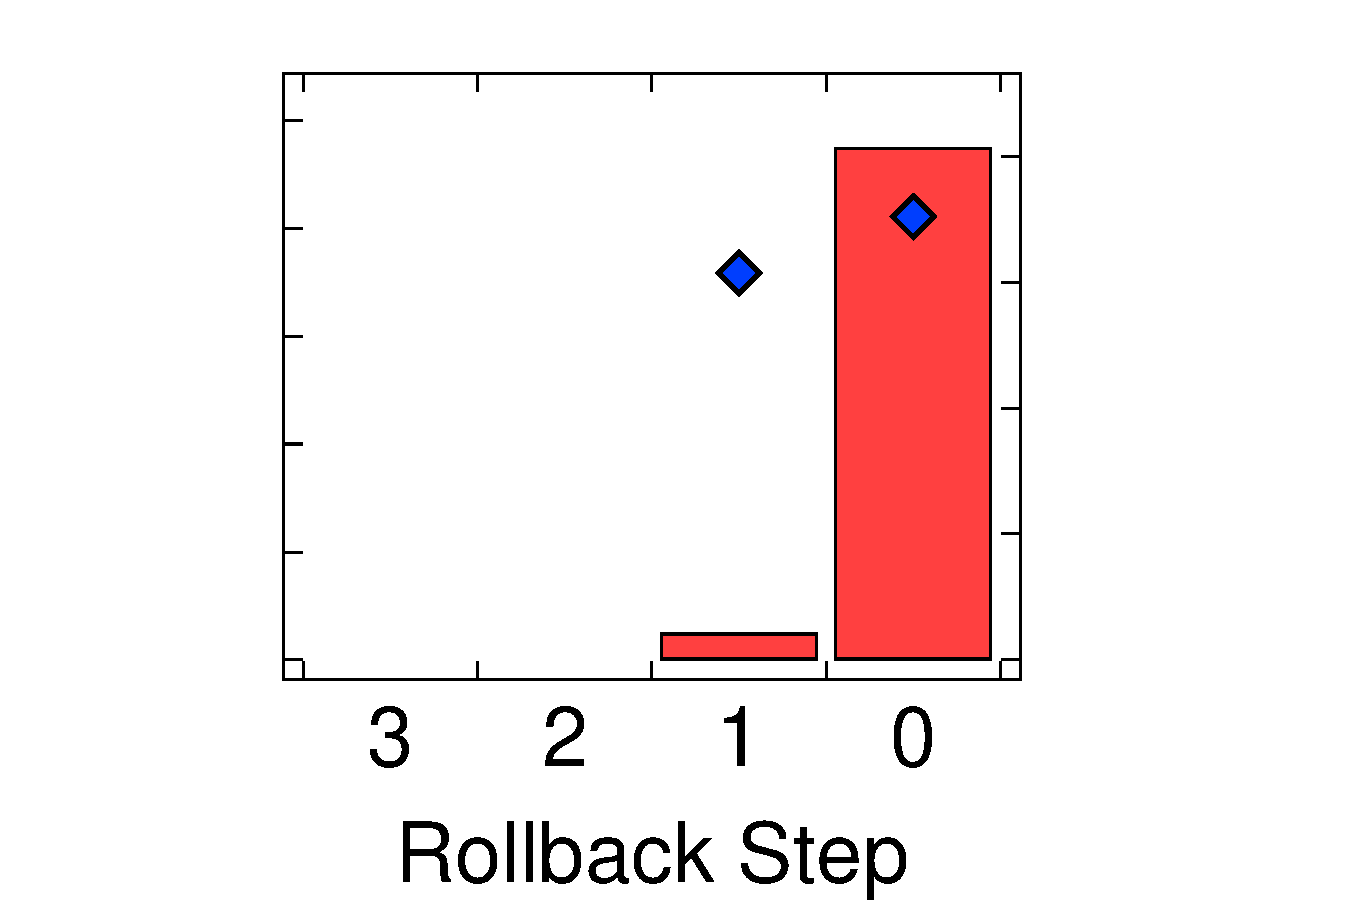
\includegraphics[trim=130 0 150 0,clip,width=\linewidth]{graphs/process/ubench-limit-dist/fp-limit-dist-p0c4.pdf}
%         \setlength{\abovecaptionskip}{-9pt}
%         \caption{P0C4, \\\bench{daxpy}}
%     \end{subfigure}
%     \hfill
%     \begin{subfigure}{.132\linewidth}
%         \includegraphics[trim=130 0 150 0,clip,width=\linewidth]{graphs/process/ubench-limit-dist/mem-limit-dist-p1c3.pdf}
%         \setlength{\abovecaptionskip}{-9pt}
%         \caption{P1C3, \\\bench{stream}}
%     \end{subfigure}
%     \hfill
%     \begin{subfigure}{.132\linewidth}
%         \includegraphics[trim=130 0 150 0,clip,width=\linewidth]{graphs/process/ubench-limit-dist/mem-limit-dist-p1c4.pdf}
%         \setlength{\abovecaptionskip}{-9pt}
%         \caption{P1C4, \\\bench{stream}}
%     \end{subfigure}
%     \hfill
%     \begin{subfigure}{.132\linewidth}
%         \includegraphics[trim=130 0 150 0,clip,width=\linewidth]{graphs/process/ubench-limit-dist/int-limit-dist-p1c5.pdf}
%         \setlength{\abovecaptionskip}{-9pt}
%         \captionsetup{oneside,margin={-4pt,0pt}}
%         \caption{P1C5, \\~~~~~\bench{coremark}}
%     \end{subfigure}
%     \hfill
%     \begin{subfigure}{.186\linewidth}
%         \includegraphics[trim=130 0 0 0,clip,width=\linewidth]{graphs/process/ubench-limit-dist/int-limit-dist-p1c7.pdf}
%         \setlength{\abovecaptionskip}{-9pt}
%         \captionsetup{oneside,margin={-4pt,27pt}}
%         \caption{P1C7, \\~~~~~\bench{coremark}}
%     \end{subfigure}
%     %\caption{For six cores, CPM inserted delay need to be rolled back from its idle limit for uBench to run correctly. The FP (\bench{daxpy}), MEM (\bench{stream}), and INT (\bench{coremark}) uBench have consistent behavior on the rolled back cores, indicating the core's idle limit is too aggressive and fails to capture some paths with long delay. The other 10 cores unshown can run uBench correctly at their idle limits.}
%     \caption{For the six cores shown above, CPM inserted delay needs to be rolled back from its idle limit for the uBench to run correctly, indicating the core's idle limit is too aggressive and fails to capture some long delay paths in the core.}
%     \label{fig:ubench-limit-dist} 
%     \vspace{-0.3cm}
% \end{figure*}


While idle system characterization reveals insights on the performance benefits and the inter-core variation issues of multicore active timing margin customization, it does not evaluate the system's behavior under stress from real-world application codes. Before using more complex applications, we use micro-benchmark (uBench) as a valuable tool that controls program behavior to analyze individual processor components~\cite{papadimitriou2018micro}. Because uBench imposes more stress than idling, the CPM configuration tends to be more conservative, creating a practical point for processor deployment in the real world.

\subsection{Workload Selection}
\label{sec:process:ubench_benchmarks}

We evaluate system behavior under aggressive active timing margin customization using three uBench programs. These programs collectively cover all main parts of the microarchitecture, as well as the dispersed CPMs in a core. 

We use \bench{coremark}~\cite{coremark} to stress the core's control, branch, and integer units; \bench{daxpy} to stress the floating point unit; and \bench{stream}~\cite{stream} for its ability to generate cache misses and exercise the load-store unit. Prior work has used such benchmarks to exercise the functional units and validate the active timing margin~\cite{lefurgy2011active, lefurgy2013active}. We check the programs' run result to evaluate processor execution correctness. All incorrect runs manifest as system crashes or abnormal application exits.

Using these benchmarks ensures we challenge a reconfigured active timing margin by touching more paths than system idle. Meanwhile, these uBench programs create little system noise, especially the $di/dt$ effect. They have controlled, smooth program behaviors and avoid complex microarchitectural activity such as periodic pipeline flush, which is the root cause of workload-induced voltage droops~\cite{grochowski2002microarchitectural,powell2003pipeline,reddi2009voltage,reddi2010voltage,miller2012vrsync}. The $di/dt$ effect is dangerous for aggressively reconfigured active timing margin because its fast drooping voltage can prevent the control loop from engaging in time~\cite{vezyrtzis2018droop}, resulting in application failure. 

\subsection{What Makes Some Cores Fail?}
\label{sec:process:ubench_profiling}

We start the uBench characterization from the idle limit because it is the point that sustains stable system state. If this initial starting point fails, the CPM inserted delay is rolled back to have a longer timing delay to make active timing margin harness timing margin more conservatively until the program runs correctly. We find most cores' idle limits sustain correct uBench execution, which entails they can safely accommodate the major paths activated by the instructions used by uBench programs. 

For the server's two physical processors, uBench characterization exposes six cores that fail for the three programs. \Fig{fig:ubench-limit-dist} shows the distributions of reintroduced delays for these cores, using the ``rollback steps'' relative to the idle limit, which reflects the stress impact from uBench program execution compared with system idle. For those six cores, rollback ranges from one to three steps and sustains all uBench workloads.

All three programs, despite their different characteristics, show similar behaviors on the six problematic cores. The implication is that the microarchitecture blocks that limit aggressive active timing margin customization are the common structures used by all programs, such as instruction fetch and scheduling, rather than specific modules stressed by each application (e.g., FP unit).

Our later analysis with a power virus and a voltage virus corroborates this conjecture. Neither of these stress tests makes the cores fails at their \textit{uBench limit}.

The power virus creates a high IR drop and high-temperature condition. At \textit{uBench limit} in \Tab{tab:limit-delay}, eight copies of \bench{daxpy} threads creates over 160~W total chip power and around 70\C chip temperature, compared with the 50\C temperature under per-core test. However, the high power does not bring any core down, verifying the robustness of \textit{uBench limit}. 

We believe this observation is intuitive because the temperature's impact on circuit speed happens over the long term, which is well within active timing margin control loop's nanosecond-level response time. A higher temperature is beneficial for circuit speed in recent technologies~\cite{zu2016tistate}, reducing concerns on high-temperature conditions.

The voltage virus creates transient voltage droops that threaten the active timing margin control loop to respond in time. We repeatedly throttle all cores' instruction issue rates to its 1/128 in synchronized step while running \bench{daxpy} to create current surges, which induces worst-case $di/dt$ effect~\cite{lefurgy2011active, lefurgy2013active}. However, under this worst-case condition, no core fails at their \textit{uBench limit}, suggesting active timing margin works fairly robustly under aggressive customization. We, therefore, use the uBench limits as a reference point for further characterization using realistic applications.

% The uBench limit is an important configuration that likely reflects the core's inherent active timing margin achievable speed because most timing paths are protected by aggressively configured active timing margin operation and real programs have high confidence of correct execution.

\section{Realistic Workload \\Characterization}
\label{sec:process:realistic}

To run real applications, a production active timing margin system today adds some amount of protection margin to CPM's uBench limit configuration~\cite{lefurgy2011active}. To conservatively guarantee execution correctness, the added margin can be up to 50\% of the static guardband. But this leaves room for improvement as demonstrated by the 2X frequency gain during our system idle characterization. 

However, adding additional guardband as a conservative precaution ignores the application-dependent behavior and can waste valuable performance benefit. In this section, we profile with a variety of integer and floating point workloads from SPEC CPU 2017~\cite{SPEC2017} and PARSEC~3.0~\cite{bienia2008parsec}. We use these workloads because their result-checking tool provides a convenient method for checking execution correctness. Understanding per core active timing margin operating limits under these heterogeneous workloads offer helpful insights for deploying aggressively customized active timing margin chips in real-world use cases.

To understand all system factors that impact an aggressively fine-tune active timing margin processor, we profile with a variety of integer and floating point workloads from SPEC CPU 2017~\cite{SPEC2017} and PARSEC~3.0~\cite{bienia2008parsec}. These realistic workloads provide helpful insight for deploying aggressively fine-tuned active timing margin chips in real-world use cases. They often have more complicated code patterns that may touch corner timing paths in a core, or introduce complex microarchitectural behaviors that can lead to severe $di/dt$ effects, both of which threaten to violate the aggressively tuned CPM configuration after uBench profiling, even though the uBench limits already ensure the active timing margin control loop protects major core paths. 

%We find that SPEC and PARSEC benchmarks usually fail at the uBench limit; this is why active timing margin processors that are deployed into the field still rely on some safety margin, approximately 50\% of the original static guardband~\cite{lefurgy2011active}, after the CPMs have been calibrated using the uBench programs. Therefore, there is still substantial room for improvement.
%The delta between each application's limit CPM configuration and the uBench limits reveal the unique impact of an application's system noise effect. Most of the workloads require that each core roll back its CPM delay from the uBench limit by at least one step to ensure execution correctness. More importantly, we observe different applications impose widely different ``stress'' levels on the aggressively configured active timing margin chip. 

\subsection{Application Heterogeneity}
\label{sec:process:workload:heterogeneity}

\begin{figure}[t]
    \subfloat[P0C3] {
        \includegraphics[trim=0 0 100 0,clip,width=0.4\linewidth]{graphs/process//spec-limit-dist/single-thread-cmp-p0c3.pdf}
        }
    \hfill
    \subfloat[P1C6] {
        \includegraphics[trim=100 0 0 0,clip,width=0.4\linewidth]{graphs/process//spec-limit-dist/single-thread-cmp-p1c6.pdf}
        }               
    \caption{\bench{x264} stresses active timing margin more heavily and needs a more conservative CPM configuration compared to \bench{gcc}, as indicated by the larger CPM rollback that is required for \bench{x264} over \bench{gcc}.}
    \label{fig:spec-limit-example} 
\end{figure}

\Fig{fig:spec-limit-example} shows \bench{x264} often requires significant CPM delay rollback from the uBench limit, whereas \bench{gcc} needs relatively little, allowing active timing margin to more aggressively boost frequency. The rollback reflects an application's unique system noise effects. Configuring active timing margin for the worst application in all cases, e.g., \bench{x264}, wastes active timing margin's margin reclamation potential when running more benign workloads. This is the approach taken by today's deployed active timing margin processors, which still rely on a safety margin as large as 50\% of the original static guardband~\cite{lefurgy2011active}. This is the case for today's active timing margin processors deployed into the field which still rely on some safety margin, approximately 50\% of the original static guardband~\cite{lefurgy2011active}.

To get a complete picture of the behavior of aggressively configured active timing margin cores on different workloads, we profile CPM rollback from the uBench limit for all $<app, core>$ pairs in \Fig{fig:app-cpm-heactive timing marginap}. We use the weighted average CPM rollback as it quantifies the application's unique stress level. Two applications may have quite a different delay reduction distributions even when they show the same lower bound in their CPM delay profile. 

From the individual rows in \Fig{fig:app-cpm-heactive timing marginap}, we see that each workload imposes a different amount of stress but does so consistently across cores. For instance, \bench{x264} and \bench{ferret} needs much more conservative active timing margin setting than \bench{gcc} and \bench{leela}, indicating these workloads have exerted a higher pressure on active timing margin's control loop.

We classify the workloads as ``heavy,'' ``medium,'' or ``light'' as shown in \Tab{tab:bench-cpm-type}. ``Heavy'' workloads pose the greatest threat to aggressively reconfigured active timing margin and often force a rollback of CPM inserted delay for more conservative operation. In contrast, ``light'' applications exert little pressure on active timing margin and often need no rollback from the uBench limit. The ``medium'' workloads show more sensitivity to a core's active timing margin control loop.

In \Tab{tab:limit-delay}, \textit{thread-worst} is the worst CPM configuration limit of all workloads and represents the most severe application stress in our profiling. The \textit{thread-normal} is less conservative and lets most medium, and light applications safely pass. From our realistic single-threaded workload profiling, we draw the following two key insights:

\begin{table}[t]
  %TODO: this table can be removed if space is needed
  \vspace{0.2cm}

  \centering
  \begin{tabular}{l|c*{2}{c}}
    \Xhline{1pt}
    stress level & benchmark \\
    \hline
    heavy  & \makecell{x264, exchange2, ferret} \\
    \hline
    medium & \makecell{perlbench, xalancbmk, xz, \\facesim, omnetpp, mcf, \\bodytrack, dedup} \\
    \hline
    light  & \makecell{gcc, bodytrack, deepsjeng, leela, \\freqmine, barnes, streamcluster, \\fluidanimate, fft, blackscholes} \\
    \Xhline{1pt}
  \end{tabular}

  \caption{Benchmark classification based on their stress level to aggressively configured active timing margin.} 
  \label{tab:bench-cpm-type} 
\end{table}

From the individual columns in \Fig{fig:app-cpm-heactive timing marginap}, we see that different cores exhibit varying levels of ``robustness'', where we define robustness as the immunity to CPM rollback from the core's CPM uBench limit. The cores on the right of~\Fig{fig:app-cpm-heactive timing marginap} has the highest robustness, requiring the least rollback across all applications, indicating their active timing margin control loops can deal with the system effects of any application. We anticipate they will continue to be robust on untested applications since the profiled workloads already cover different behaviors~\cite{song2018spec}.

The reason why certain applications and cores are more vulnerable after aggressive active timing margin customization is a combination of the core's inherent speed and the running application's characteristics. We conducted a best-effort static instruction analysis on the applications and concluded that more detailed insight into the running instructions is needed to predict each application's best-fit CPM setting on each core. For instance, \bench{gcc} covers a much richer set of instructions than \bench{exchange2}, likely touching more corner timing paths, yet stresses active timing margin much less. As another example, \bench{x264} has similar performance counter profiles as \bench{leela}, but their rollback requirements differ substantially. We, therefore, defer the root-cause analysis and the prediction of applications' heterogeneous CPM configuration to future work and focus on the variations already exposed.

\begin{figure}[t]
  \centering
  \includegraphics[trim=0 0 0 0,clip,width=\linewidth]{graphs/process//spec-limit-dist/app-rollback.png}
  \caption{Application's average CPM delay rollback from the core's uBench limit. The top workloads stress active timing margin heavily and need more delay rollback for less aggressive margin reclamation.}
  \label{fig:app-cpm-heactive timing marginap}
\end{figure}

\subsection{Core Robustness Heterogeneity}
\label{sec:process:workload:robustness}

%Looking horizontally in~\Fig{fig:app-cpm-heactive timing marginap}, different cores, cores exhibit varying active timing margin control ``robustness''---under complex workload-induced system noise, the amount of CPM delay needed to roll back from the core's inherent speed which is exposed by the uBench limit profile. In \Fig{fig:app-cpm-heactive timing marginap}, the cores on the right exhibit the highest robustness because they need the least rollback across all applications, indicating their active timing margin control loops can deal with the system effect caused by whatever application fairly well. 

Cores have varying levels of ``robustness'' to application heterogeneity, where we define robustness as the immunity to CPM rollback from the core's inherent speed (the uBench limit profile). From the columns in \Fig{fig:app-cpm-heactive timing marginap}, the cores on the right exhibit the highest robustness, requiring the least rollback across all applications, indicating their active timing margin control loops can deal with the system effects of any application.

\Fig{fig:core-cpm-var} sorts cores' average rollbacks across all workloads. The rightmost cores, P0C7, P1C2, and P1C7 are immune to workload effects, flawlessly executing all applications at their uBench limit. We anticipate they will continue to be robust on untested applications since the profiled workloads already cover various behaviors~\cite{song2018spec}. These ``robust cores'' can be relied upon in a production environment to execute any application. Among the robust cores, P1C7, however, is notable because its CPM delay was rolled back from the idle test to the uBench test, significantly reducing its frequency to a rather conservative 4800~MHz, possibly accounting for its apparent robustness. Contrariwise, P0C7 remains robust even at its CPM delay from the idle test. As such, there is no clear correlation between a core's speed and its active timing margin robustness. 

%To favor execution reliability, the cores that have more robust active timing margin operation on the right side of \Fig{fig:core-cpm-var} have higher priority for running applications.

\Fig{fig:core-cpm-var} also summarizes different cores' frequency variation under the profiled scenarios. At the uBench limit configuration, core-to-core speed varies by 300~MHz from the fastest, P0C6, to the slowest, P1C7. The speed gap shrinks to 200~MHz at the thread-worst limit, caused by CPM delay rollback of the non-robust active timing margin cores. Nevertheless, the non-uniform core frequency is still impressive and deserves proper management.
%If alternatively selected to favor performance, faster cores should be given higher priority for running applications.

\begin{figure}[t]
  \centering
  \includegraphics[trim=0 20 0 20,clip,width=\linewidth]{graphs/process//spec-rollback.pdf}
  \caption{Aggressively configured active timing margin cores exhibit different CPM rollback steps and frequencies when running realistic workloads.}
  \label{fig:core-cpm-var}
\end{figure}

\section{Managing active timing margin in the Field}
\label{sec:process:schedule}


In this section, we discuss how to manage a customized active timing margin system's performance in the presence of core-to-core variation as well as application heterogeneity. Overall, application performance is improved by customized active timing margin's elevated frequency level. However, the varying frequency levels for each core, and each application creates trouble for the processor in delivering a promised performance level to end users. Hence, we show how to schedule applications and make performance promises to latency sensitive applications.


%To manage active timing margin's performance variability, we first develop a predictor that informs frequency and performance for a candidate application schedule (\Sec{sec:schedule:predict}). Then we propose an active timing margin-aware scheduler to manage application performance improvement with deterministic behavior (\Sec{sec:schedule:framework}). We evaluate its effectiveness (\Sec{sec:schedule:result}).

\subsection{Performance Variability}

 \begin{figure}[t]
  \centering
      \includegraphics[trim=0 0 0 0,clip,width=.75\linewidth]{graphs/process/schedule-space.pdf}
      \captionsetup{width=.9\linewidth}
      \caption{Aggressive ATM customization expose wide frequency variation, causing performance unpredictability.}
      \label{fig:schedule-space}
\end{figure}

Under the conventional static margin setting, all cores are shipped with a single, fixed frequency of 4.2~GHz. The default active timing margin system tries to match this goal with a uniform boosted performance around 4.6~GHz, as shown by the ``default (sys idle)'' bar in~\Fig{fig:schedule-space}. The default CPM setting smooth core-to-core variation to a limited 50~MHz, as illustrated by the max and min frequencies. 

But when aggressively customizing each core's active timing margin setting to maximize performance, system operators must learn to manage core-to-core performance variation carefully. active timing margin customization exposes the core-to-core performance variation while boosting performance to over 4.9~GHz. The frequency variation is over 200~MHz between cores even when no application is running, as shown by the ``customized (sys idle)'' bar. 

At runtime, the frequency variation is further complicated because workloads consume a different amount of power, which induces varying levels of DC voltage drop along the chip's shared power delivery path. DC voltage drop decreases the supply voltage delivered to the transistors and erodes the timing margin, limiting the frequency gain available for active timing margin's control loop~\cite{zu2015adaptive}. 

Running eight copies of \bench{daxpy} raises power consumption by 60~W and drops a customized core's frequency to 4.5~GHz, as shown by the min freq of ``customized (workload).'' Though this is still much better than the static margin, the performance delivered to an application is much slower than the max frequency setting, which is over 5.0~GHz when idle. 

Hence, system operators that are deploying customized active timing margin system need to be careful when scheduling applications and making performance promises.


\subsection{Per-core Frequency Predictor}
\label{sec:process:schedule:predict}

To manage active timing margin's performance variability, we first develop a predictor that informs frequency and performance for a candidate application schedule. We develop this predictor by modeling each core's runtime average frequency $\overline{f}$, as a linear function of the transistors' supply voltage, $V_{chip}$. Among different dynamic effects, long-term stable effects such as temperature variation and DC voltage drop caused by high power determines core frequency ---infrequent, transient $di/dt$ events are handled transparently by the active timing margin control loop. 

\begin{figure}[t]
  \centering
      \includegraphics[trim=0 0 0 0,clip,width=.75\linewidth]{graphs/process/freq-pred.pdf}
      \captionsetup{width=.9\linewidth}
      \caption{After ATM customization, core frequency can be predicted with a fitted linear model, following \Eq{eq:freq-pred}.}
\label{fig:freq-pred}
\end{figure}

Because past research has shown that speed is only modestly affected by temperature~\cite{zu2016tistate}, we base our model strictly on IR voltage drop. Subtracting the IR voltage drop, which is proportional to current and hence power consumption, we derive a linear relationship between active timing margin's dynamic frequency and the chip's total power consumption as shown in  \Eq{eq:freq-pred}. The value $b$ represents a core's static CPM setting, while $k' \cdot \overline{P}$ represents the dynamic variation, dominated by the IR voltage drop. 

\begin{equation}\label{eq:freq-pred}
\begin{split}
\overline{f} &= k \cdot \overline{V_{chip}} = k \cdot (V_{vrm} - R \cdot \overline{I})\\
&= k \cdot (V_{vrm} - R \cdot \frac{\overline{P}}{V_{vrm}})\\
&= -k' \cdot \overline{P} + b
\end{split}
\end{equation}

\Fig{fig:freq-pred} shows the linear model fitted for each core's customized CPM configuration. The measured data points align with \Eq{eq:freq-pred}'s predictions. Each additional watt degrades the frequency by about two MHz. In practice, each core stores its frequency prediction model and the model is indexed by the chip's total power consumption during job scheduling and runtime.

\subsection{Delivering Critical App's Performance}
\label{sec:process:schedule:framework}

\begin{figure}
  \centering
      \includegraphics[trim=0 0 0 0,clip,width=.7\linewidth]{graphs/process/perf-pred.pdf}
      \captionsetup{width=.9\linewidth}
      \caption{Single-thread application performance can be predicted linearly using core frequency.}
\label{fig:1t-perf-pred}
\end{figure}

Frequency directly affects application performance. \Fig{fig:1t-perf-pred} shows application performance scales linearly with frequency, with different coefficients depending on the workload's memory behavior. A memory-bound workload, such as \bench{mcf}, enjoys less performance improvement from higher frequency compared with a compute-bound workload like \bench{x264} because cache misses limits the compute throughput. We, therefore, build a performance predictor for each application, using frequency as the input. In this way, thread performance on each core can be inferred by the chip's total power, using each core's frequency predictor as the intermediate step.

On a customized active timing margin system, each application's performance depends on both the core it runs on as each core has different CPM configuration which leads to varying frequency levels, and the applications running on other neighboring cores, as all applications contribute to the chip's total power which in turn affects each core's frequency through the DC voltage drop on the shared power delivery path. For some \texttt{critical} applications that the users are interested in, it is crucial that they get mapped to the customized cores that are high performance and robust. Meanwhile, it is also crucial that the co-located \texttt{background} applications are adequately managed so that the total chip power does not exceed the level that hampers critical app's core frequency. To handle this issue, we propose a scheme to selectively throttle \texttt{background} application performance to control total chip power, and indirectly frees up frequency potential for \texttt{critical} applications.

\begin{table}[h!]
  \centering
  \resizebox{\columnwidth}{!}{
  \begin{tabular}{c|c|c}
    \Xhline{1pt}

    Mem behavior      & Critical & Background \\
    \hline
    Intensive  & \makecell{resnet, vgg,\\ ferret, \\fluidanimate} & \makecell{mlp, gcc,\\facesim, lu\_cb, \\streamcluster, etc.} \\
    \hline
    Non-intensive  & \makecell{squeezenet, \\seq2seq, babi, \\bodytrack, vips} & \makecell{blackScholes, x264, \\swaptions,\\ raytrace, } \\
    \Xhline{1pt}
  \end{tabular}
    }

  \caption{Classifying critical and background applications, based on their memory subsystem interference behavior.} 
  \vspace{-0.2cm}

  \label{tab:bench-type} 
\end{table}

We use the applications in \Tab{tab:bench-type} for evaluation. The \texttt{critical} workloads are user-facing and require high performance for lower latency. They include deep learning inference (CNN, RNN, and LSTM models), object detection, real-time image processing, content similarity search, etc. The \texttt{background} workloads can tolerate lower performance and include workloads such as stock price estimation, 3D image rendering, compression, compilation, and machine learning training. For our work, we focus on the performance issue caused by the active timing margin system's shared power delivery problem and excludes performance interference from the memory subsystem which is a general issue for all multicores. Thus, we avoid co-locating two memory-intensive workloads at the same time to simplify the problem.

\begin{sidewaysfigure}
  \centering
  \includegraphics[trim=10 90 10 150,clip,width=\linewidth]{graphs/process//schedule-flow/schedule-flow.pdf}
  \caption{Managing a customized active timing margin system needs to integrate the per-app performance predictor and per-core frequency predictor, so that \texttt{critical} application performance can be satisfied by using faster cores and maintaining an estimated chip power budget.}
  \label{fig:schedule-flow}
\end{sidewaysfigure}

\Fig{fig:schedule-flow} outlines our management scheme. It takes into account the core-to-core performance and robustness variation as characterized in~\Sec{sec:realistic}, and the inter-core application power interference on the power delivery subsystem. First, the user selects how he/she would like to set different core's CPM. The default policy uses the chip's thread-worst CPM configuration as shown in \Tab{tab:limit-delay}, obtained through our earlier characterization.

The default thread-worst policy represents a balanced trade-off between performance and reliability. Most likely workloads can execute correctly while still providing better performance. The \texttt{critical} and \texttt{background} workloads all execute correctly under thread-worst.

For higher performance, the user selects an ``aggressive'' governor, which chooses an application's most aggressive CPM configuration that guarantees correct execution. In the current approach, this can be achieved by repetitive profiling an application's CPM limits in a tier of testing servers before shipping the application to production server clusters. For most medium and light workloads in~\Tab{tab:bench-type}, thread-normal represents the high-performance policy.

For higher robustness, the user can select a ``conservative'' governor, which only schedules \texttt{background} workloads onto robust cores picked by active timing margin characterization. The robust cores are scarce and may not provide the highest performance, but they have the highest guarantee of correct execution. The conservative policy is best for unknown applications or when application correctness is paramount.

The operating system then automatically sets each core's CPM setting according to user-selected policy. The faster cores after CPM customization are selected for running \texttt{critical} application. In parallel with CPM reconfiguration, the scheme reads user-specified QoS target for the \texttt{critical} application and infers the chip power needed to meet the performance goal using per-application performance predictor and per-core frequency predictor. To meet the QoS goal, total chip power under \texttt{critical} and co-running \texttt{background} workloads cannot exceed the calculated power budget.

The manager subtracts the estimated power of the \texttt{critical} workloads from the total chip power budget to get the power envelope available for the co-running \texttt{background} jobs. The \texttt{background} jobs can then be scheduled to the same chip under this envelope by carefully tuning their power consumption. On POWER7+ where $V_{dd}$ is shared for all cores, we adjust power consumption by changing core frequency. Depending on the power envelope, we can 1)~allow workloads to use aggressive active timing margin that has the highest frequency, 2)~set cores to different DVFS states' frequency levels or 3)~use power-gating to disable cores.

\subsection{Performance Improvement}
\label{sec:process:schedule:result}

%We show in \Fig{fig:schedule-1t-results} the performance benefits provided by our scheduler to \texttt{fg} jobs in an aggressive active timing margin system. To study the impact of co-located jobs on a multi-core chip, we restrict execution to P0 of our two-socket system. We restrict the foreground job to a single core (possibly utilizing its SMT capabilities), which is a natural fit for many applications, such as LSTM and RNN inference.
%We evaluate the performance benefit of latency critical \texttt{fg} jobs in aggressive active timing margin systems in \Fig{fig:schedule-1t-results}. We co-locate all workloads onto P0 of our two-socket system to study the impact of co-located \texttt{bg} jobs on a multi-core. To highlight frequency's impact on job performance, we restrict \texttt{fg} job to use one core, which is natural for many applications, such as LSTM and RNN inference.

We evaluate our solution(s) against the static margin and the default active timing margin. Some customers turn off active timing margin for predictability. Hence the static margin is one of the fair baselines we compare with for evaluation. The system is running the stock DVFS operating system governors that already strive to improve system efficiency. Therefore, our results include that comparison implicitly. Since active timing margin systems are still new and rare, there is little other prior work to compare against directly.

Our evaluation is carried out when all cores are scheduled to run an application. In practice, power gating idle cores off when not enough workloads are available can further free up chip power and boost the performance of target workload~\cite{zu2015adaptive}. For all our tests, die temperature is maintained under 70\C, and no side effect on-chip cooling is observed. 

\begin{sidewaysfigure}
  \centering
  \includegraphics[trim=10 30 0 0,clip,width=\linewidth]{graphs/process//schedule-1t.pdf}
  \caption{\texttt{Critical} application performance co-located with \texttt{background} workloads under different settings, shown as $<\!critical:background\!>$ pairs. Aggressively customized active timing margin, together with low-power co-running \texttt{background} workloads, boosts performance by 15.4\% on average. With proper management, a 10\% performance improvement goal is guaranteed for \texttt{critical workloads} by throttling co-runner's core frequency to main total chip power below budget.}
  \label{fig:schedule-1t-results}
\end{sidewaysfigure}

\Fig{fig:schedule-1t-results} summarizes the performance benefit of managing an aggressively customized active timing margin system. To highlight frequency interference's impact, we use one core to run \texttt{critical} application, which is a natural fit for many applications, such as LSTM and RNN inference. We co-locate all \texttt{critical} and \texttt{background} applications on processor 0 (P0) of our two-socket server.

Under static margin, the default DVFS governor makes POWER7+ processors clock at fixed 4.2~GHz to run applications, providing predictable but low performance. 

The default active timing margin improves performance uniformly for all cores, not with the highest efficiency. An unmanaged system ignores the sensitivity of core frequency to total chip power. active timing margin may be indiscriminately activated on all cores, both for \texttt{critical} and \texttt{background} workloads, which significantly raises total chip power, eroding timing margin and reducing all cores' frequency, thereby diminishing the \texttt{critical} application performance. This unmanaged system still increases frequency thanks to active timing margin's harnessed margin, but the improvement is restricted to only 6.1\% on average.

Aggressively customized active timing margin provides more frequency gain, but an unmanaged system prevents the processor from providing maximum benefit. Compared with the default active timing margin, an unmanaged processor system may carelessly assign the slowest core after CPM reconfiguration to a \texttt{critical} job, limiting the peak performance that can be achieved. The unmanaged system may also let all co-located \texttt{background} workloads run under their highest frequency, increasing total chip power and reducing \texttt{critical} workload frequency. However, in this scenario \texttt{critical} applications still enjoy 10.2\% improvement over static margin because customizing active timing margin unlocks substantial frequency gain.

A managed active timing margin system can opt to maximize the performance of \texttt{critical} applications. Specifically, \texttt{critical} applications get assigned to the fastest cores, and \texttt{background} application power is minimized by applying the lowest p-state. In this way, \texttt{critical} application frequency is maximized, at the cost of \texttt{background} workload performance. On average, \texttt{critical} workload performance improves by 15.2\%.

Alternatively, a managed active timing margin system can opt to balance \texttt{critical} and \texttt{background} jobs by letting \texttt{critical} applications just meet their performance goal, and maximizing \texttt{background} performance under that promise. Suppose the user targets 10\% performance improvement for a \texttt{critical} workload over the static margin run, our managed system then throttles \texttt{background} core frequencies with the minimal amount to control total chip power, letting the frequency of the core running \texttt{critical} workload reach the level that delivers target performance.

In \Fig{fig:schedule-1t-results} the performance of \bench{squeezenet}, \bench{ferret}, \bench{vgg19}, and \bench{fluidanimate} exceeds the 10\% improvment target when the chip aims at maximizing their performance. However, their performance drops below the target when the chip puts all cores into customized active timing margin states. A balanced point can be obtained by controlling \texttt{background} workload frequency. In this case, the frequency of co-located \bench{lu\_cb}, \bench{raytrace}, \bench{swaptions}, and \bench{x264} is set to the 4.2~GHz p-state.

On the contrary, \bench{seq2seq} outperform the 10\% improvement goal when its co-located \bench{streamcluster} runs under customized active timing margin. This is because \bench{streamcluster} consumes little power even when the frequency is high. The extra available power budget can be exploited by swapping \bench{streamcluster} with a more power-hungry co-runner, \bench{lu\_cb}, with core frequency properly throttled. 

The other \texttt{critical} and \texttt{background} workloads combinations meet the QoS target when active timing margin is aggressively customized for all cores. The high-frequency gain of active timing margin customization provides this benefit. For these cases, no core throttling needs to take place.

In summary, core-level active timing margin customization and active timing margin-aware application power management provide 5\% to 10\% steady performance improvement over the original active timing margin system. This result is notable because the improvement comes on a production-grade system where even a 1\% performance gain is considered significant.

\section{Related Work}
\label{sec:process:related}

There is a plethora of work on process variation, inter-core performance heterogeneity, and multicore scheduling~\cite{liang2007process,sarangi2008varius,teodorescu2008variation,rangan2009thread,dighe2010within,rangan2011achieving}. We leverage ATM's capability of tracking a core's inherent speed and do not need prior knowledge on the core's max frequency. Our proposal for core-level ATM customization conveniently expose the inter-core performance heterogeneity and help users leverage it.

Prior art has shown multi-core performance interference through the memory subsystem~\cite{mars11micro,tang11isca,delimitrou2014quasar,lo2015heracles,verma2015large,llull2017cooper}. Our work is the first to show that on an ATM system, the shared power delivery subsystem introduces a new dimension of resource contention, and proper management is required to reap ATM's full performance benefits in a predictable way.

